%
%
%
%
\section{Rotor Unsteady Flow Analysis}
\label{rt27_unsteady.sec}
\headb{Transonic Turbine Stage}{Rotor unsteady flow analysis}
%
%
 In this section unsteady results obtained using the linear
 frequency domain approach are presented. First, the sources of unsteadiness
 obtained from the NGV outlet steady-state solution are discussed.
 Potential- and vortical-rotor interactions were evaluated for the first
 two tangential Fourier modes and the superimposed results
 compared with the available experimental data.
 Sections \ref{rt27_vortical.subsec} and \ref{rt27_potential.subsec}
 present a physical interpretation of the two type unsteady interactions, i.e.
 potential and vortical.
 As reported in Appendix \ref{waves.chap}, there is a third type of unsteady
 interaction caused by the entropy variation across the NGV wake. This interaction
 produces unsteady pressure variations which are of one order of magnitude
 less then those obtained from the potential and vortical NGV non-uniformities.
 For this reason the entropy mode is included in the vortical mode, also associated
 with the NGV-wake.
 This means that the total unsteady flow-filed in the rotor passage is given by the
 superimposition of the potential and vortical modes.
%
%
%
%
\subsection{Sources of unsteadiness}
\label{rt27_sources.subsec}
%
%
 The sources of unsteadiness in the rotor passage are represented by the
 steady-state tangential non-uniformities at the outflow boundaries
 of the stator blade.
 Such non-uniformities, which can be assumed to
 be approximately steady in the stator frame of reference, are unsteady
 in the rotor frame of reference since the rotor is moving
 through them.
%
%
\begin{figure}
 \begin{center}
  \begin{tabular}{c}
    \subfigure[Dimensionless static pressure]
       {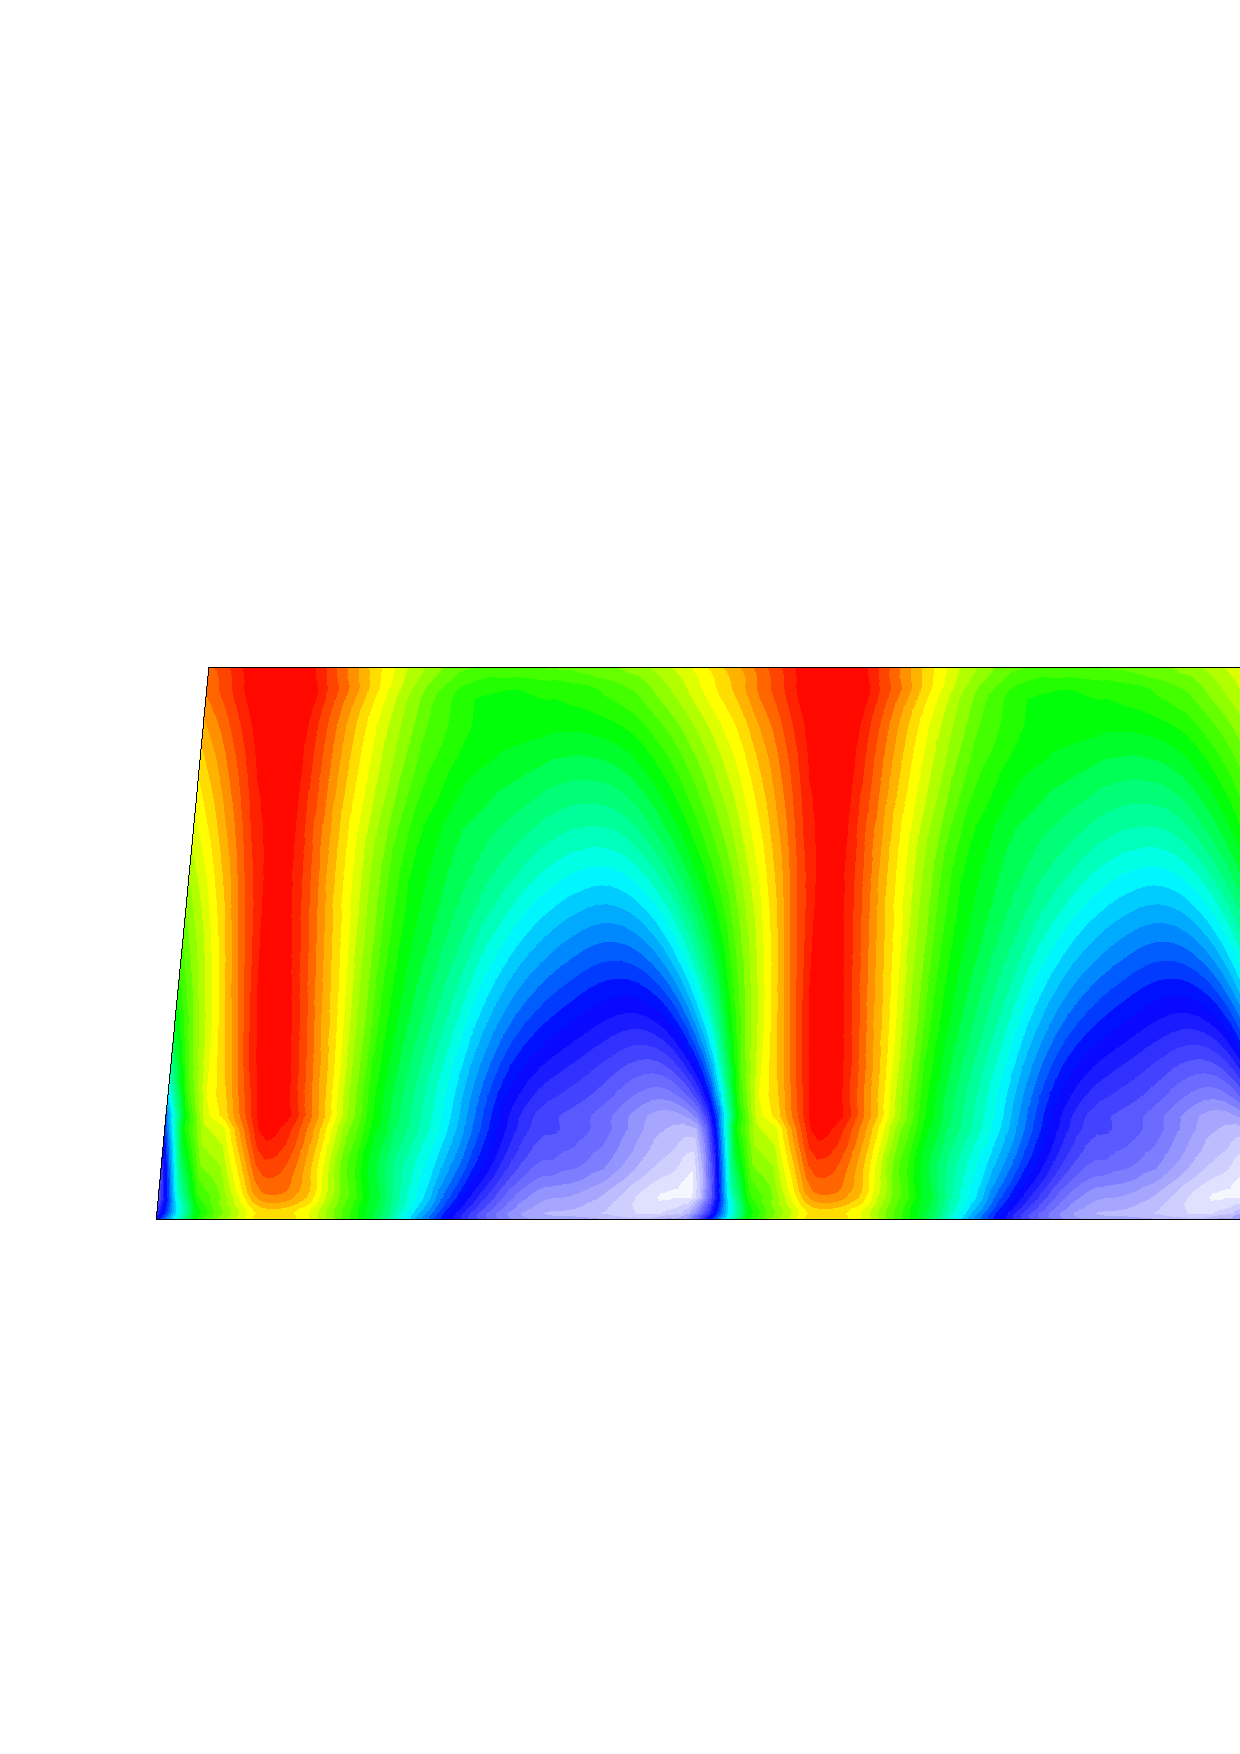
\includegraphics[width=130mm,clip=t]{CHAP_RT27/FIGURE/ngvout_pres.pdf}}
      \vspace{-2mm}\\
    \subfigure[Mach number]
       {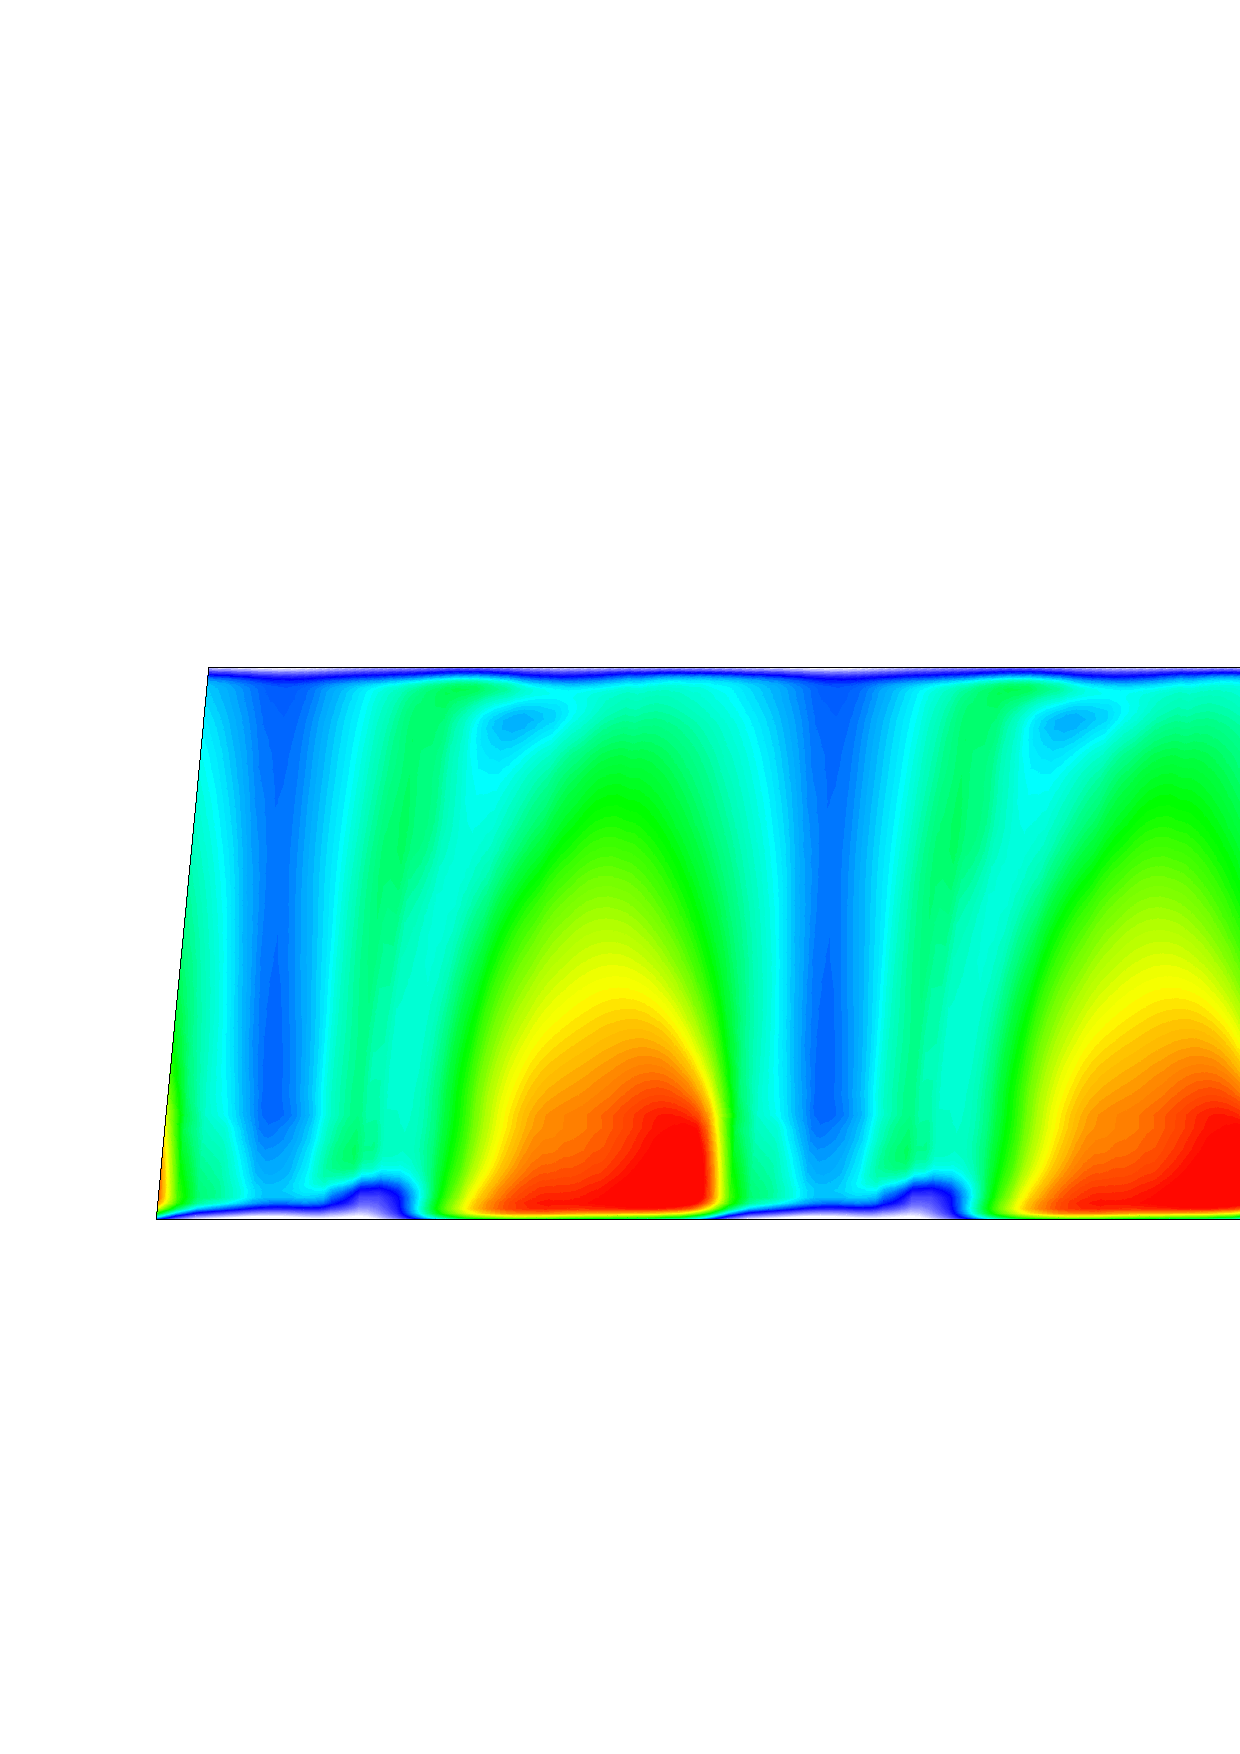
\includegraphics[width=130mm,clip=t]{CHAP_RT27/FIGURE/ngvout_mach.pdf}}
      \vspace{-2mm}\\
    \subfigure[Dimensionless total pressure]
       {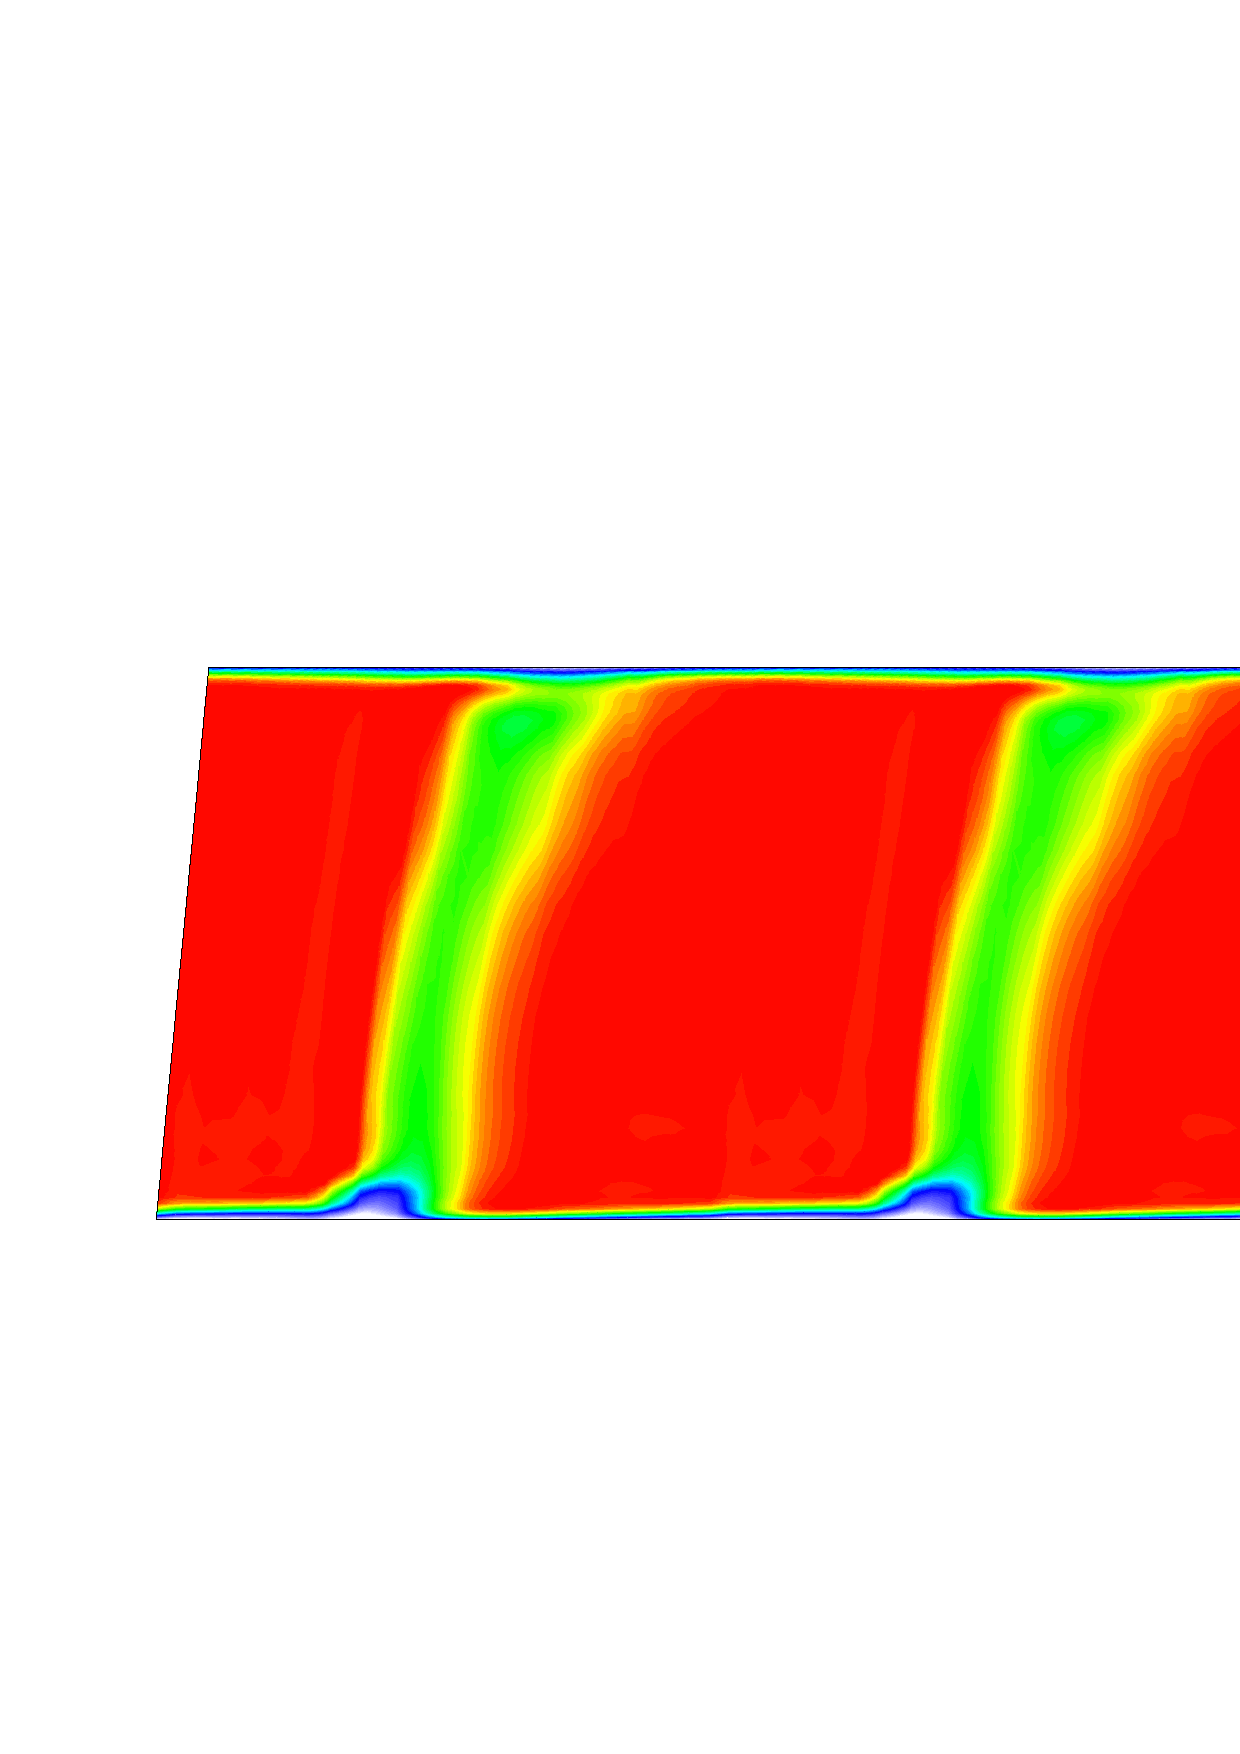
\includegraphics[width=130mm,clip=t]{CHAP_RT27/FIGURE/ngvout_ptot.pdf}}
  \end{tabular}
 \end{center}
 \vspace{-8mm}
 \caption{Steady state solution at the RT27a NGV outlet boundary (2 passages)}
 \label{ngv_outlet_solution.fig}
\end{figure}
%
 Fig. \ref{ngv_outlet_solution.fig} shows the computed steady-state
 solution at the NGV outlet. The static pressure distribution shows a
 weak shock wave towards the hub section where the average outlet Mach number
 is just above unity.
 The Mach number contours in Fig. \ref{ngv_outlet_solution.fig}b
 show the potential field associated with the static pressure contours
 but the wake profile is not evident apart from the hub
 section of the blade where the wake seems to have a quite strong
 radial variation.
 The total pressure contours, on the other hand, clearly exhibit the
 wake structure which appears to run almost radially, with the exception of
 the root region.
%
\begin{figure}
 \begin{center}
  \begin{tabular}{c}
    \subfigure[Vortical component of dimensionless absolute velocity]
        {\begin{tabular}{cc}
        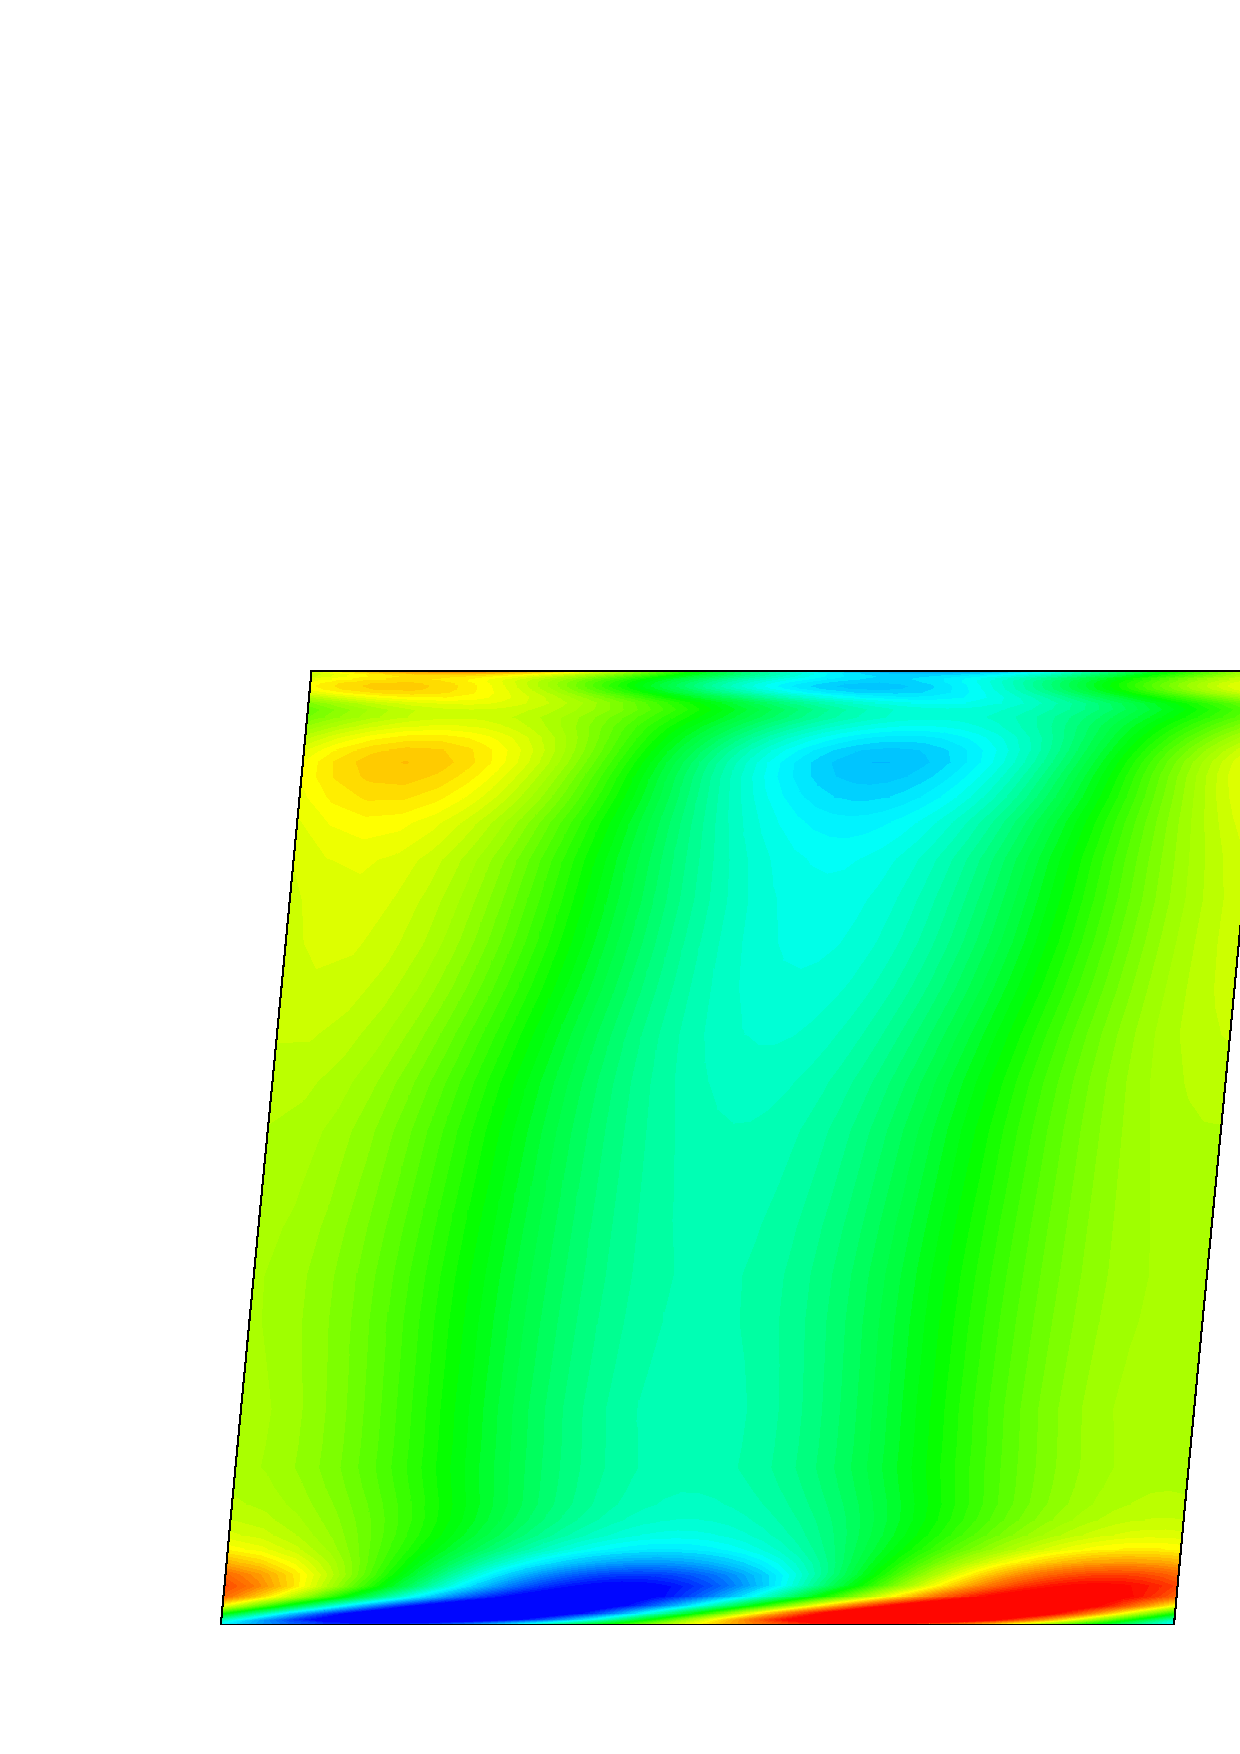
\includegraphics[width=70mm,clip=t]{CHAP_RT27/FIGURE/out_vort1.pdf}
        &
        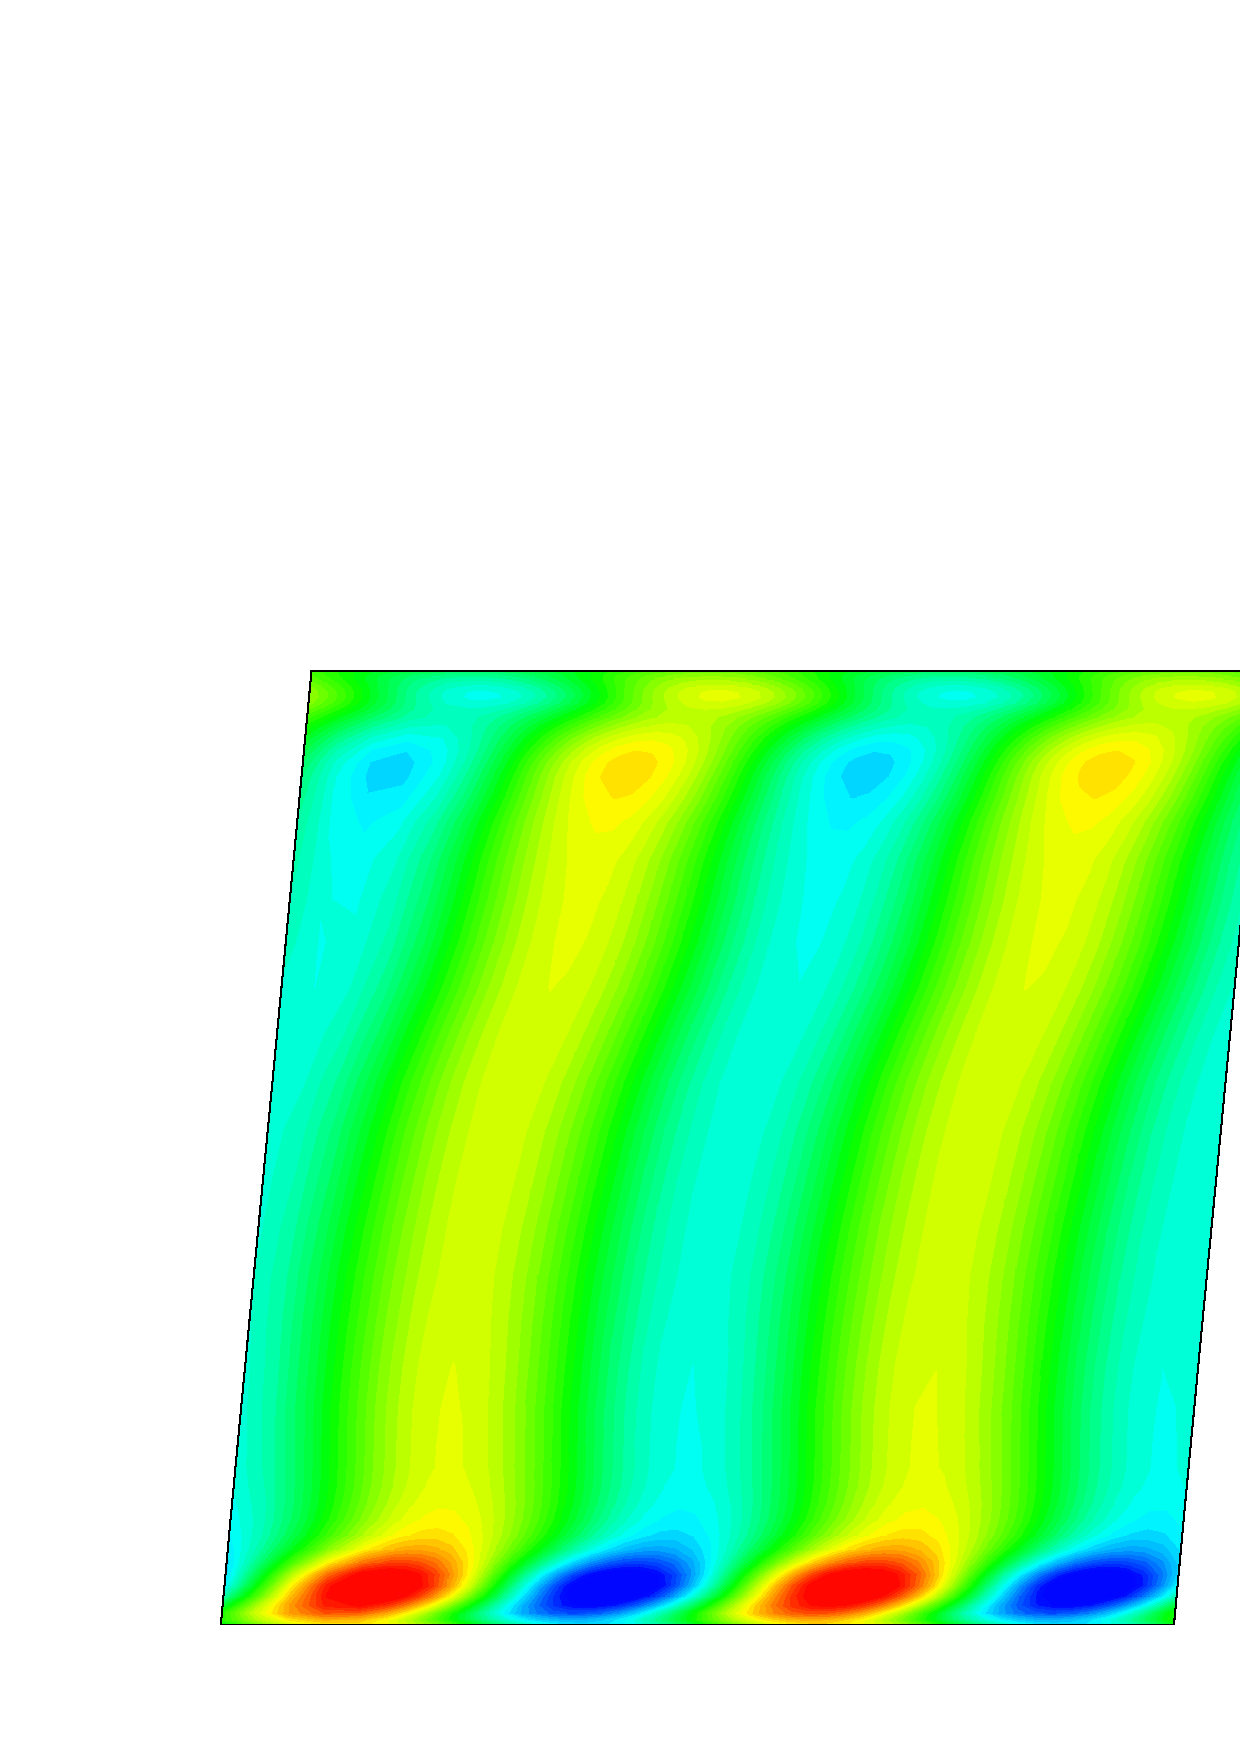
\includegraphics[width=70mm,clip=t]{CHAP_RT27/FIGURE/out_vort2.pdf}
        \end{tabular}}
    \vspace{-2mm}\\
    \subfigure[Dimensionless pressure]
        {\begin{tabular}{cc}
        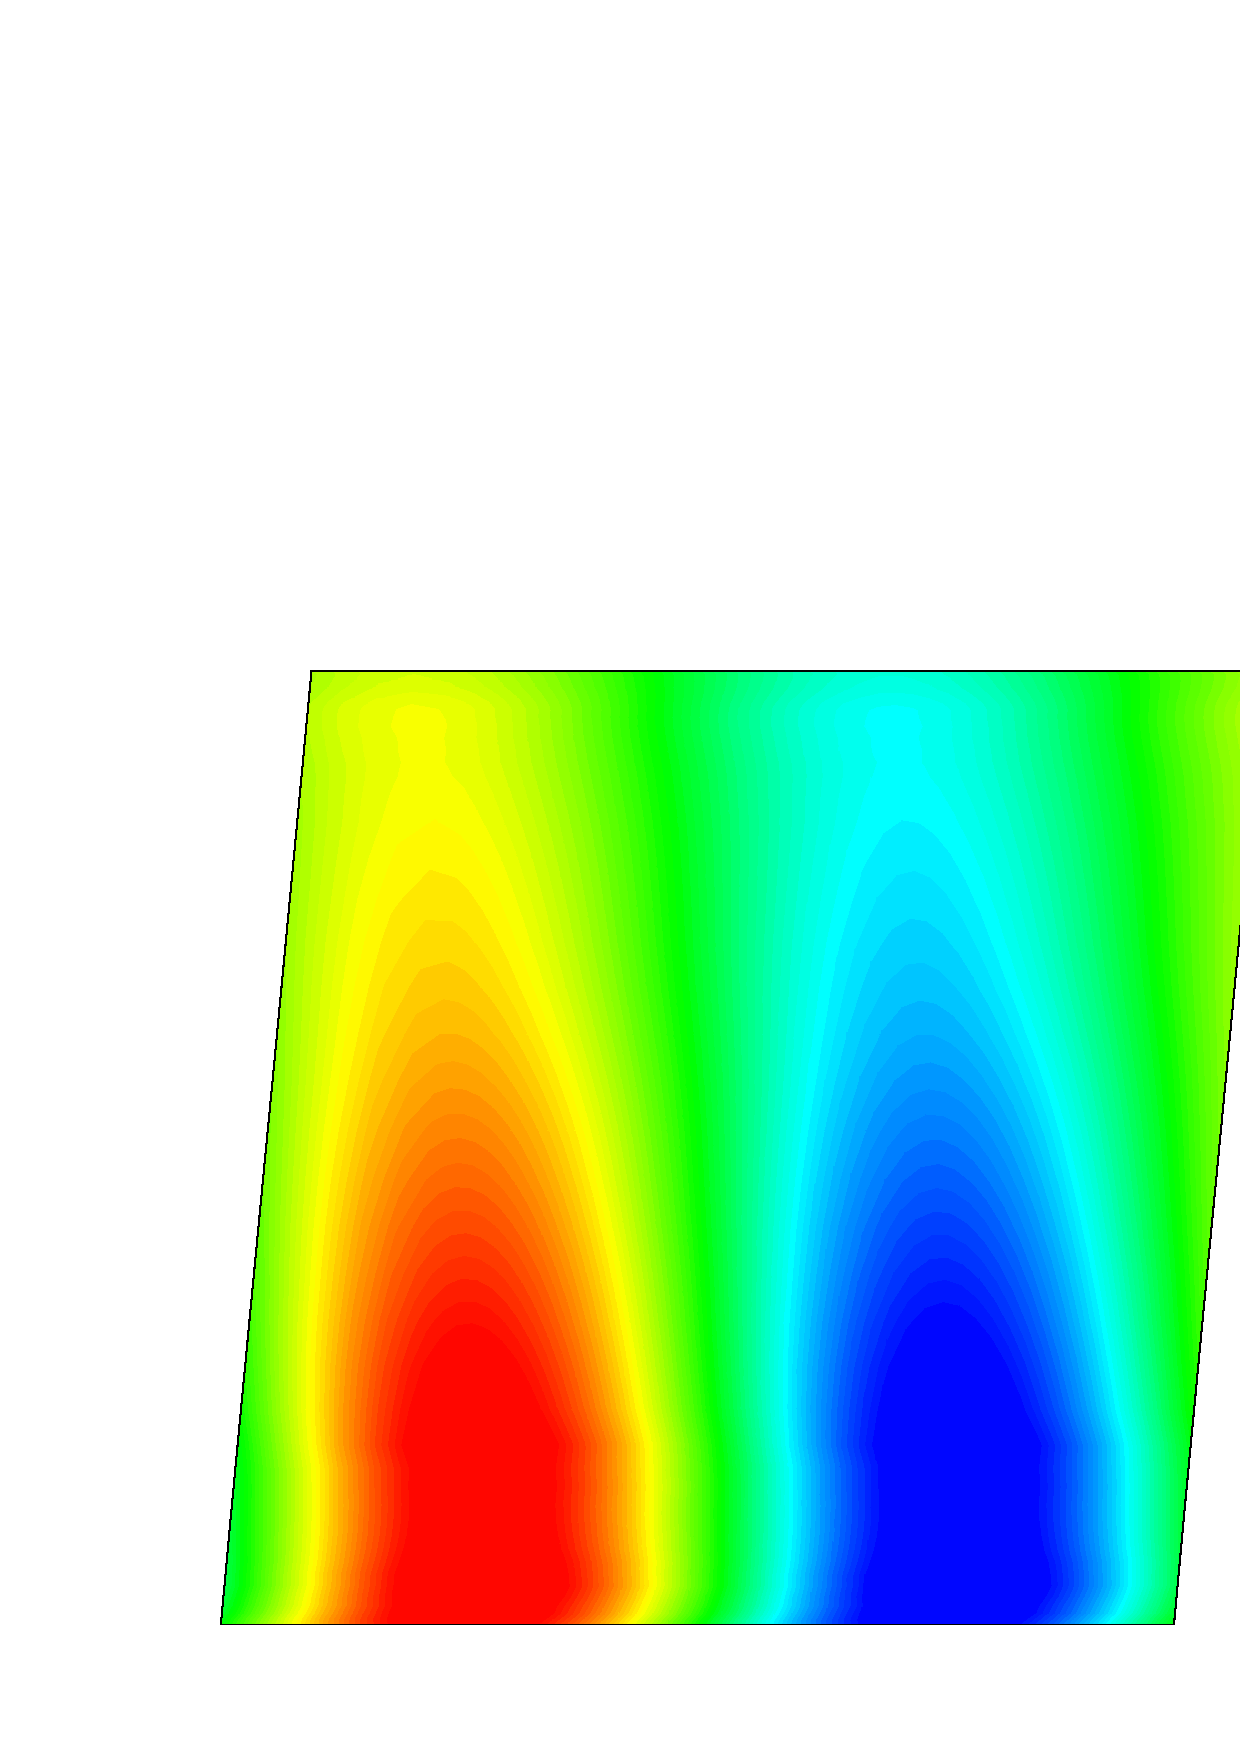
\includegraphics[width=70mm,clip=t]{CHAP_RT27/FIGURE/out_pote1.pdf}
        &
        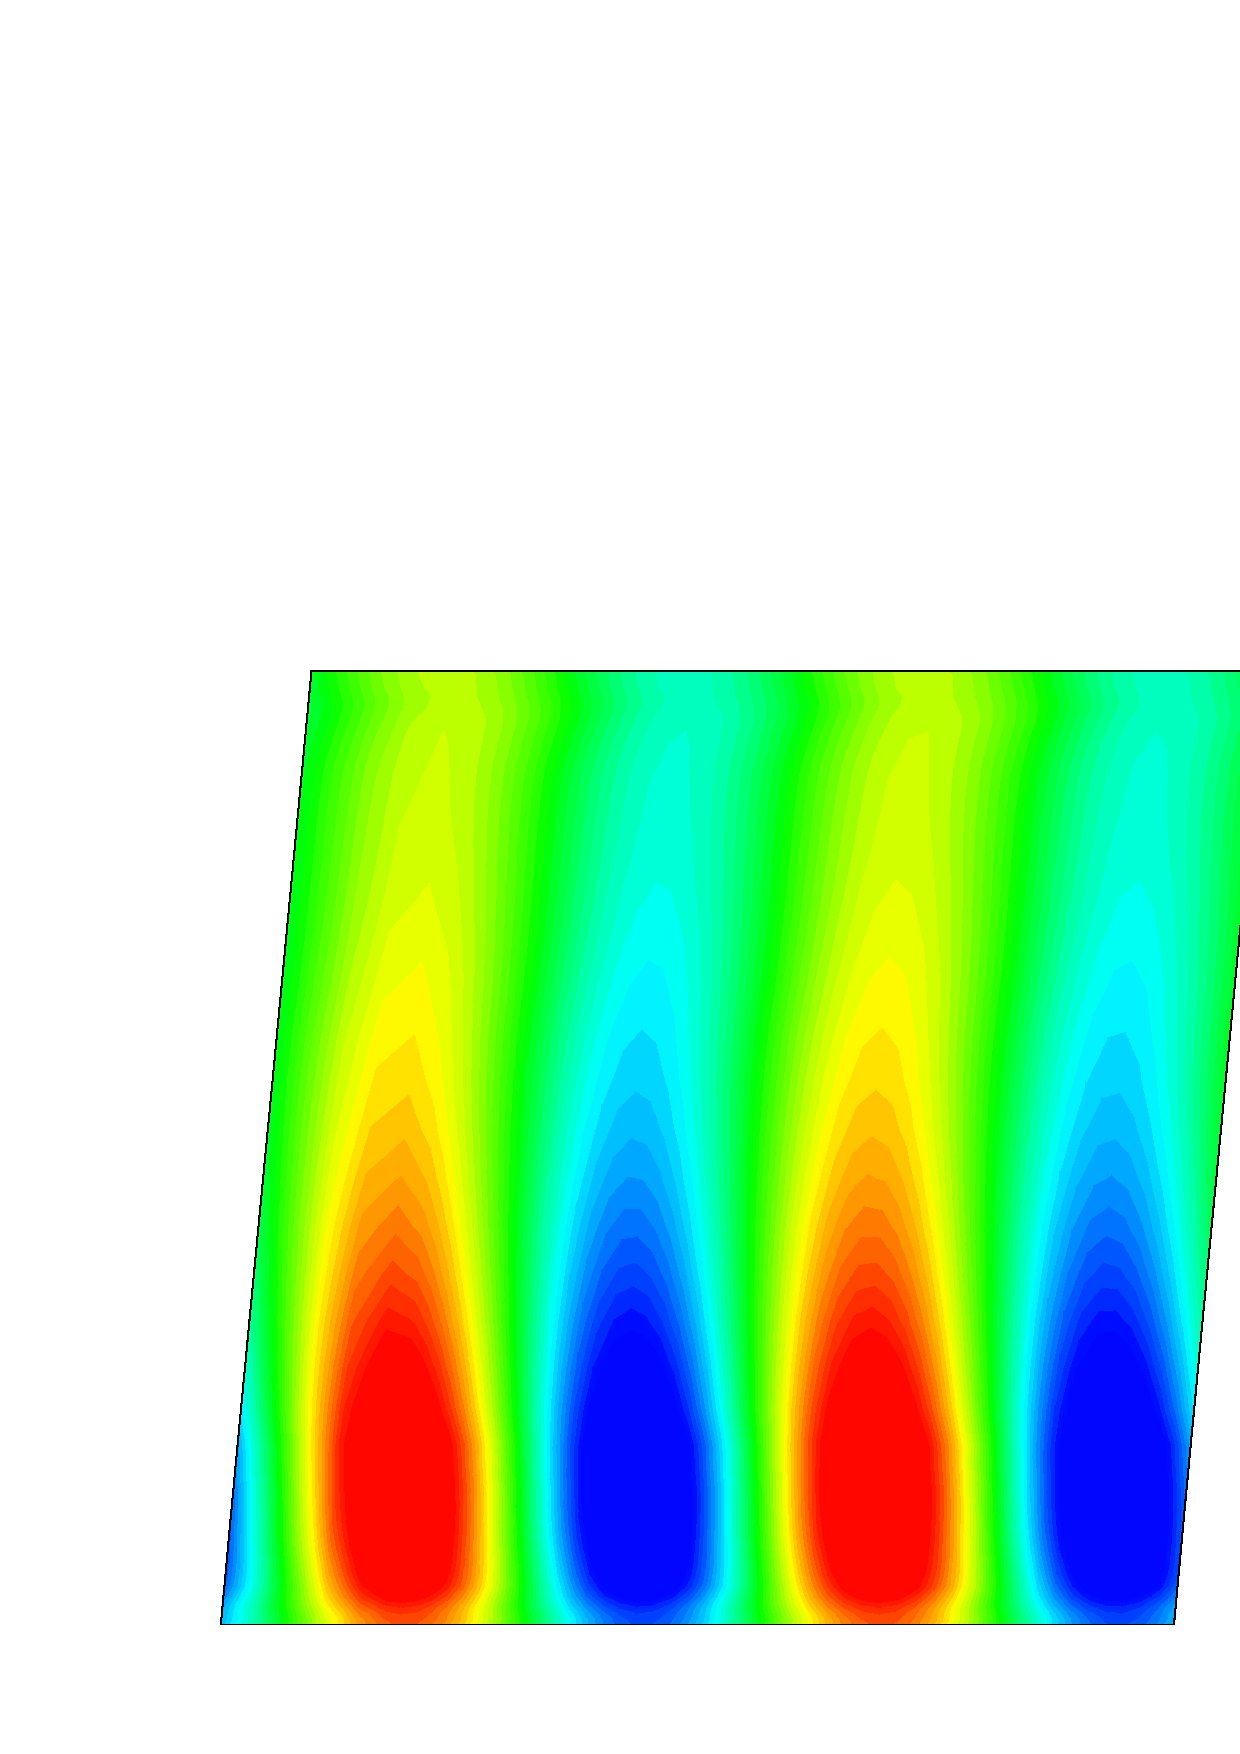
\includegraphics[width=70mm,clip=t]{CHAP_RT27/FIGURE/out_pote2.pdf}
        \end{tabular}}
    \vspace{-2mm}\\
    \subfigure[Entropic component of dimensionless density]
        {\begin{tabular}{cc}
        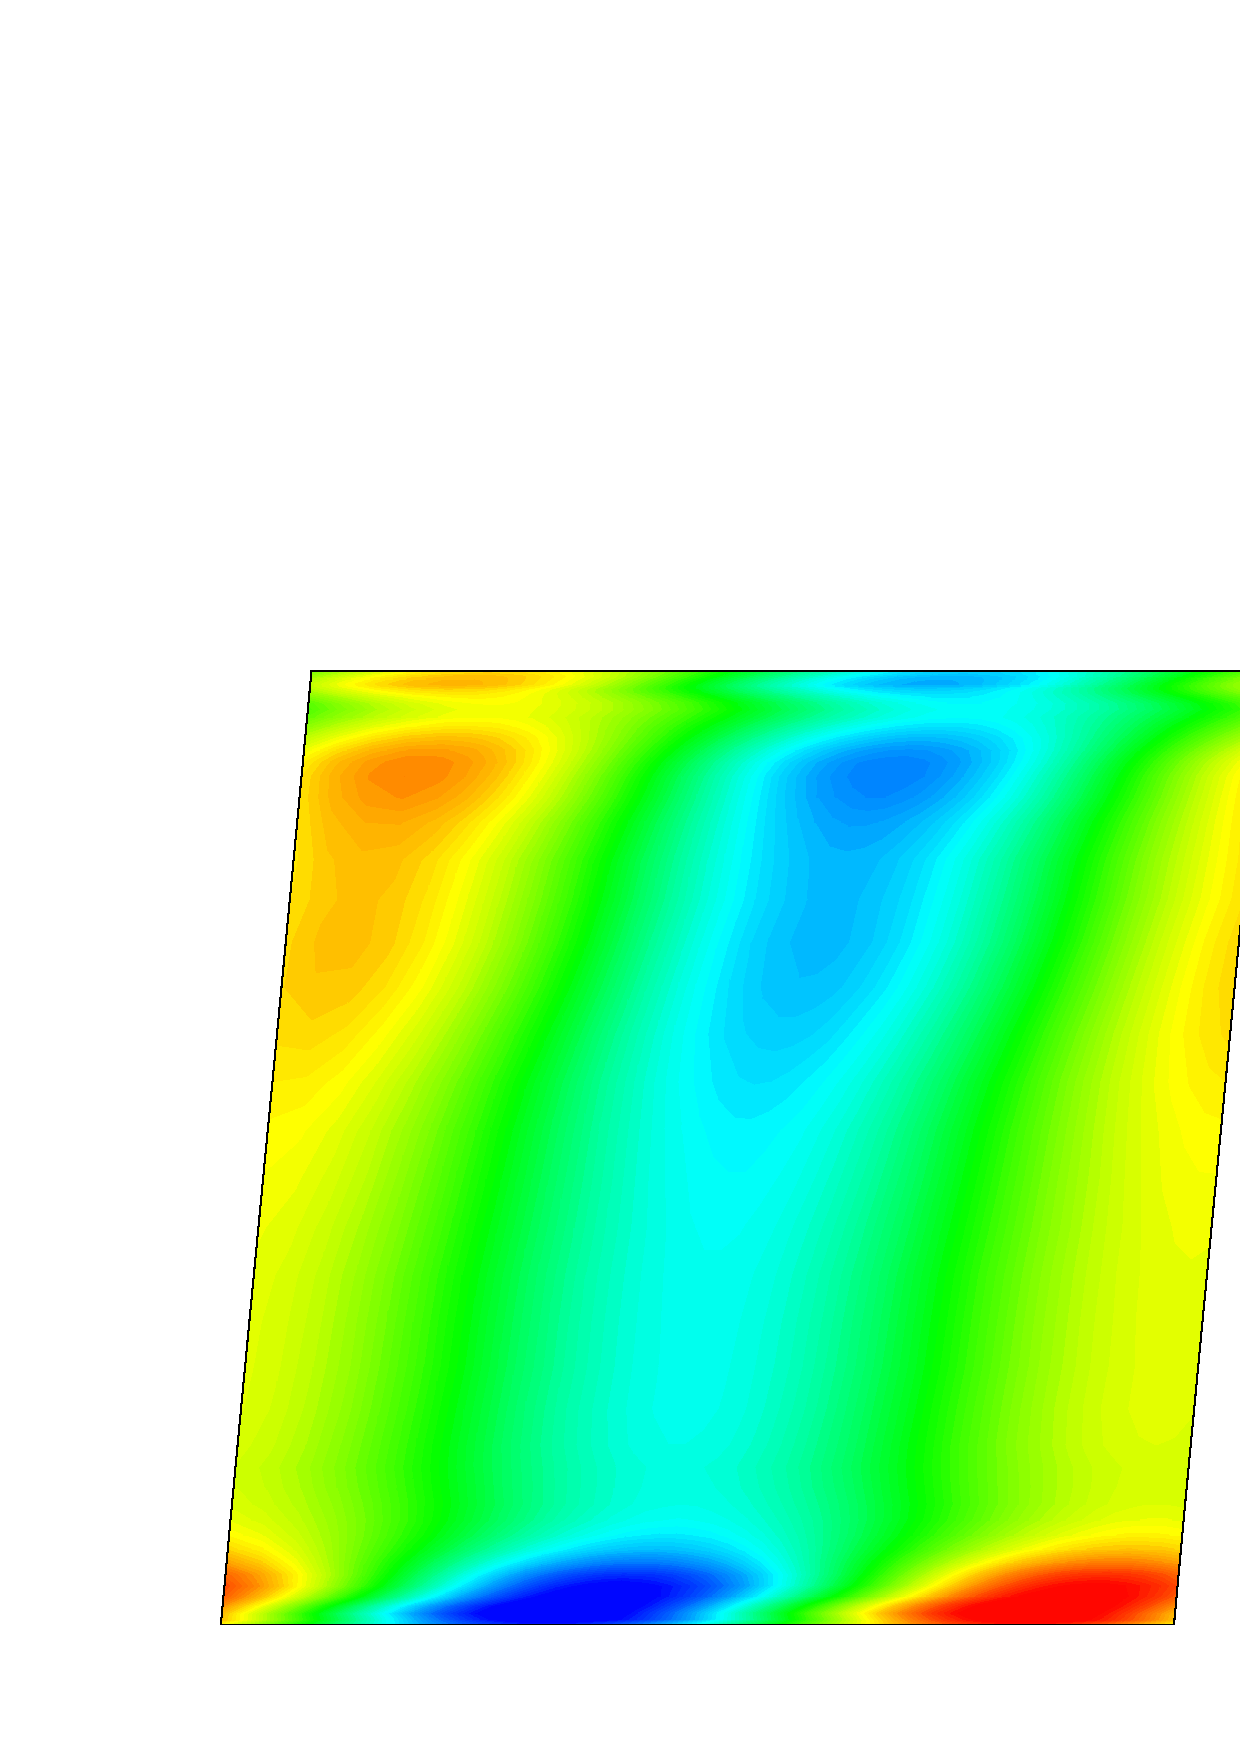
\includegraphics[width=70mm,clip=t]{CHAP_RT27/FIGURE/out_entr1.pdf}
        &
        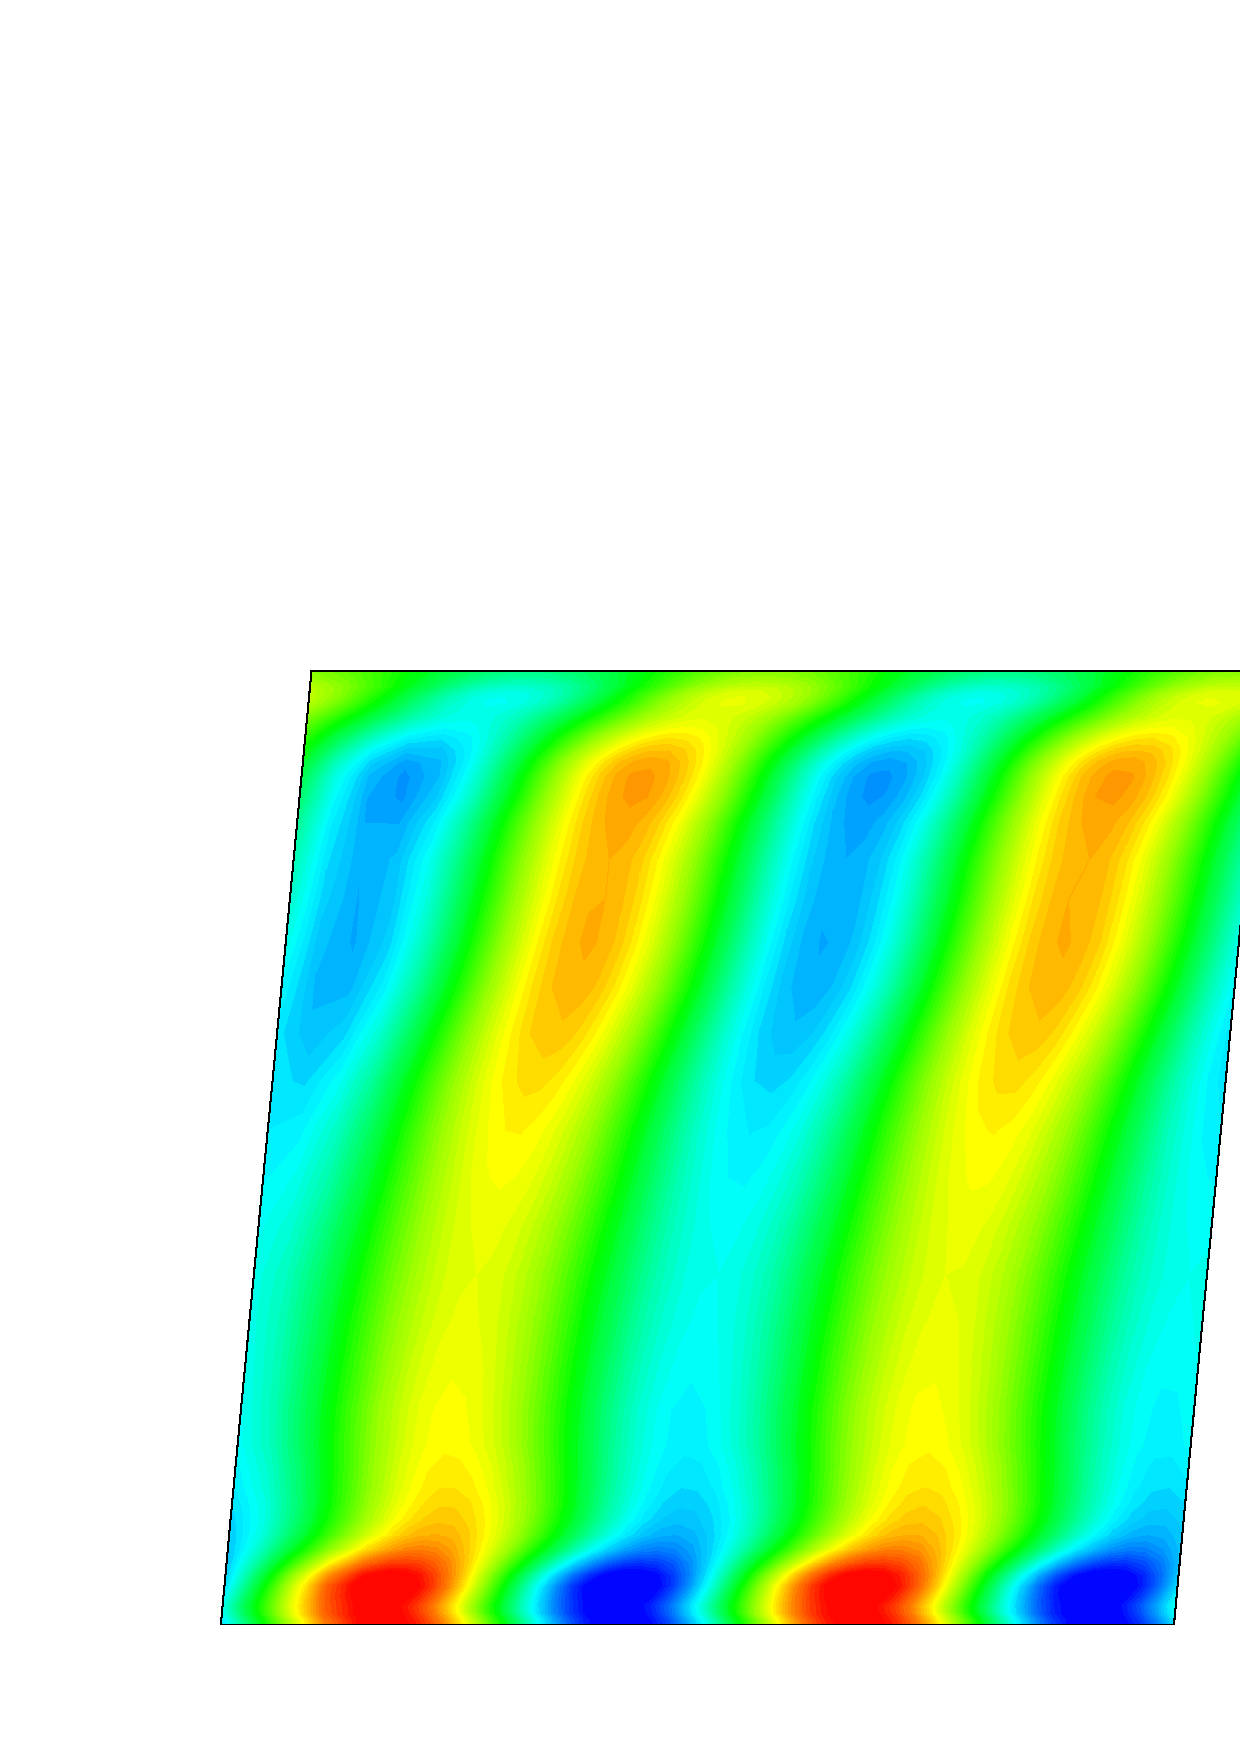
\includegraphics[width=70mm,clip=t]{CHAP_RT27/FIGURE/out_entr2.pdf}
        \end{tabular}}
    \end{tabular}
 \end{center}
 \vspace{-8mm}
 \caption{First (left) and second (right) Fourier components
          of spatial non-uniformities of RT27a NGV outlet solution (1 passage)}
 \label{ngv_outlet_decomposed1.fig}
\end{figure}
%
%
%
 The rotor blades move through the steady NGV-outlet from left to right of
 Fig. \ref{ngv_outlet_solution.fig} and they see the spatial non-uniformities
 as unsteady perturbations.
 Such spatial non-uniformities are periodic in the tangential coordinate
 and they can be decomposed into Fourier components for each radial section.
 The unsteady velocities contain two parts: a rotational (vortical) part, associated
 with the NGV wake, and an irrotational (potential) part associated with pressure
 variations. In the same way, the unsteady density contains two parts: an entropic
 part associated with the NGV wake and an irrotational (potential) part, again
 associated with the pressure variation.
 Such a grouping means that each Fourier mode of the steady flow solution at the
 NGV outlet can be seen as summation of three different modes:
 vortical, potential and entropic.
 Appendix \ref{waves.chap} shows how to calculate
 such modes for each Fourier harmonic using Goldstein's splitting theorem
 and the linearised acoustic equations.

 The vortical component of the spatial non-uniformities is associated with
 velocity variations with zero divergence and hence with
 the velocity defect in the NGV wake.
 Fig. \ref{ngv_outlet_decomposed1.fig}a shows the first two Fourier components
 of the absolute velocity variations associated with the vortical component.
 The first harmonic, usually referred as `gust'
 (Manwaring \& Wisler \citeyearNP{Manwaring:1}), clearly shows the
 three-dimensionality of the NGV-wake towards the root section. Very large
 velocity deficit occurs half a cycle or so earlier that the
 mid-height wake. Such wake inclination was also measured by Moss et al.
 \citeyear{Moss:1}.
 Fig. \ref{ngv_outlet_decomposed1.fig}b shows the pressure perturbation
 which is associated only with the potential field of the NGV outlet.
 Neither Fourier component has strong 3D features.
 The first two harmonics of the density perturbation associated with
 the entropic mode are shown in Fig. \ref{ngv_outlet_decomposed1.fig}c.
%
%
%
\begin{figure}
 \begin{center}
  \begin{tabular}{cc}
    \subfigure[Vortical component]
       {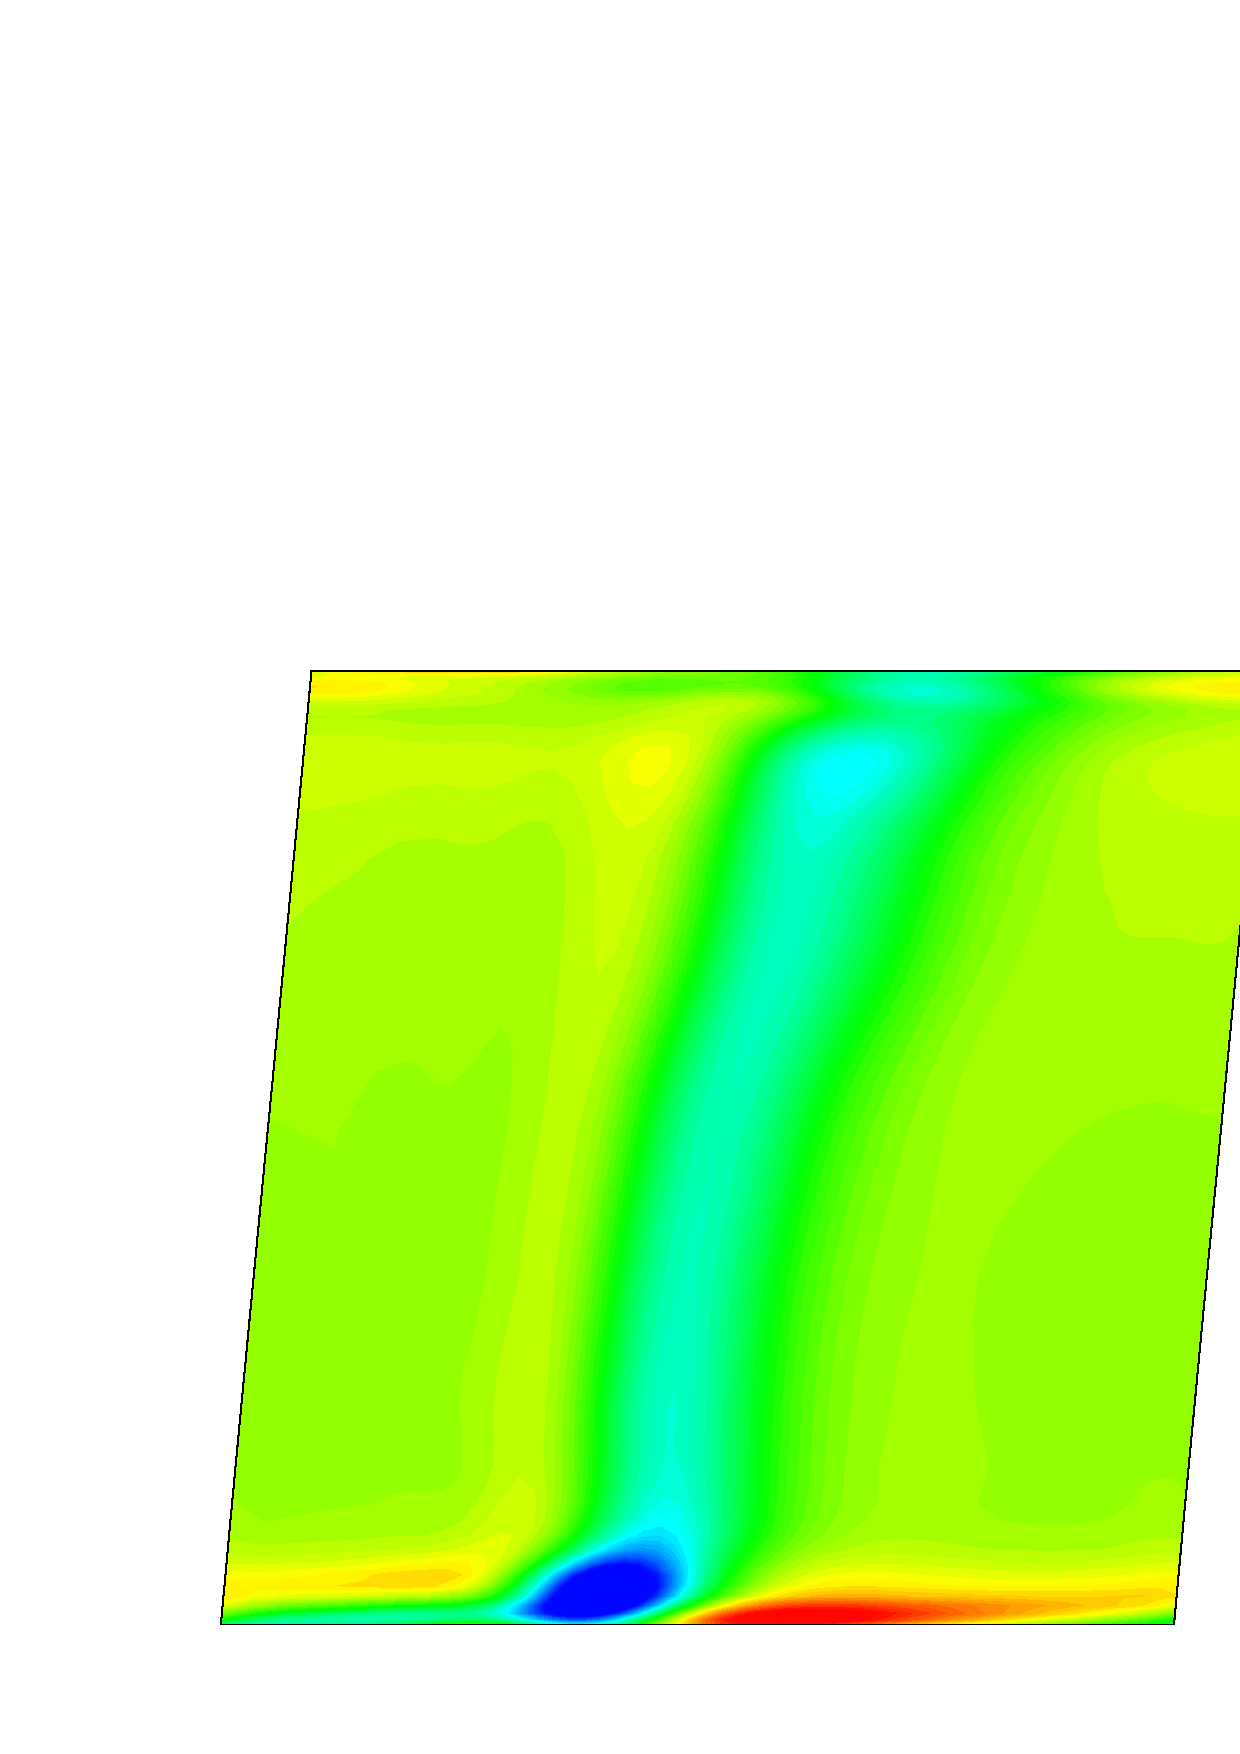
\includegraphics[width=70mm,clip=t]{CHAP_RT27/FIGURE/out_vel_vor.pdf}}
      &
    \subfigure[Potential component]
       {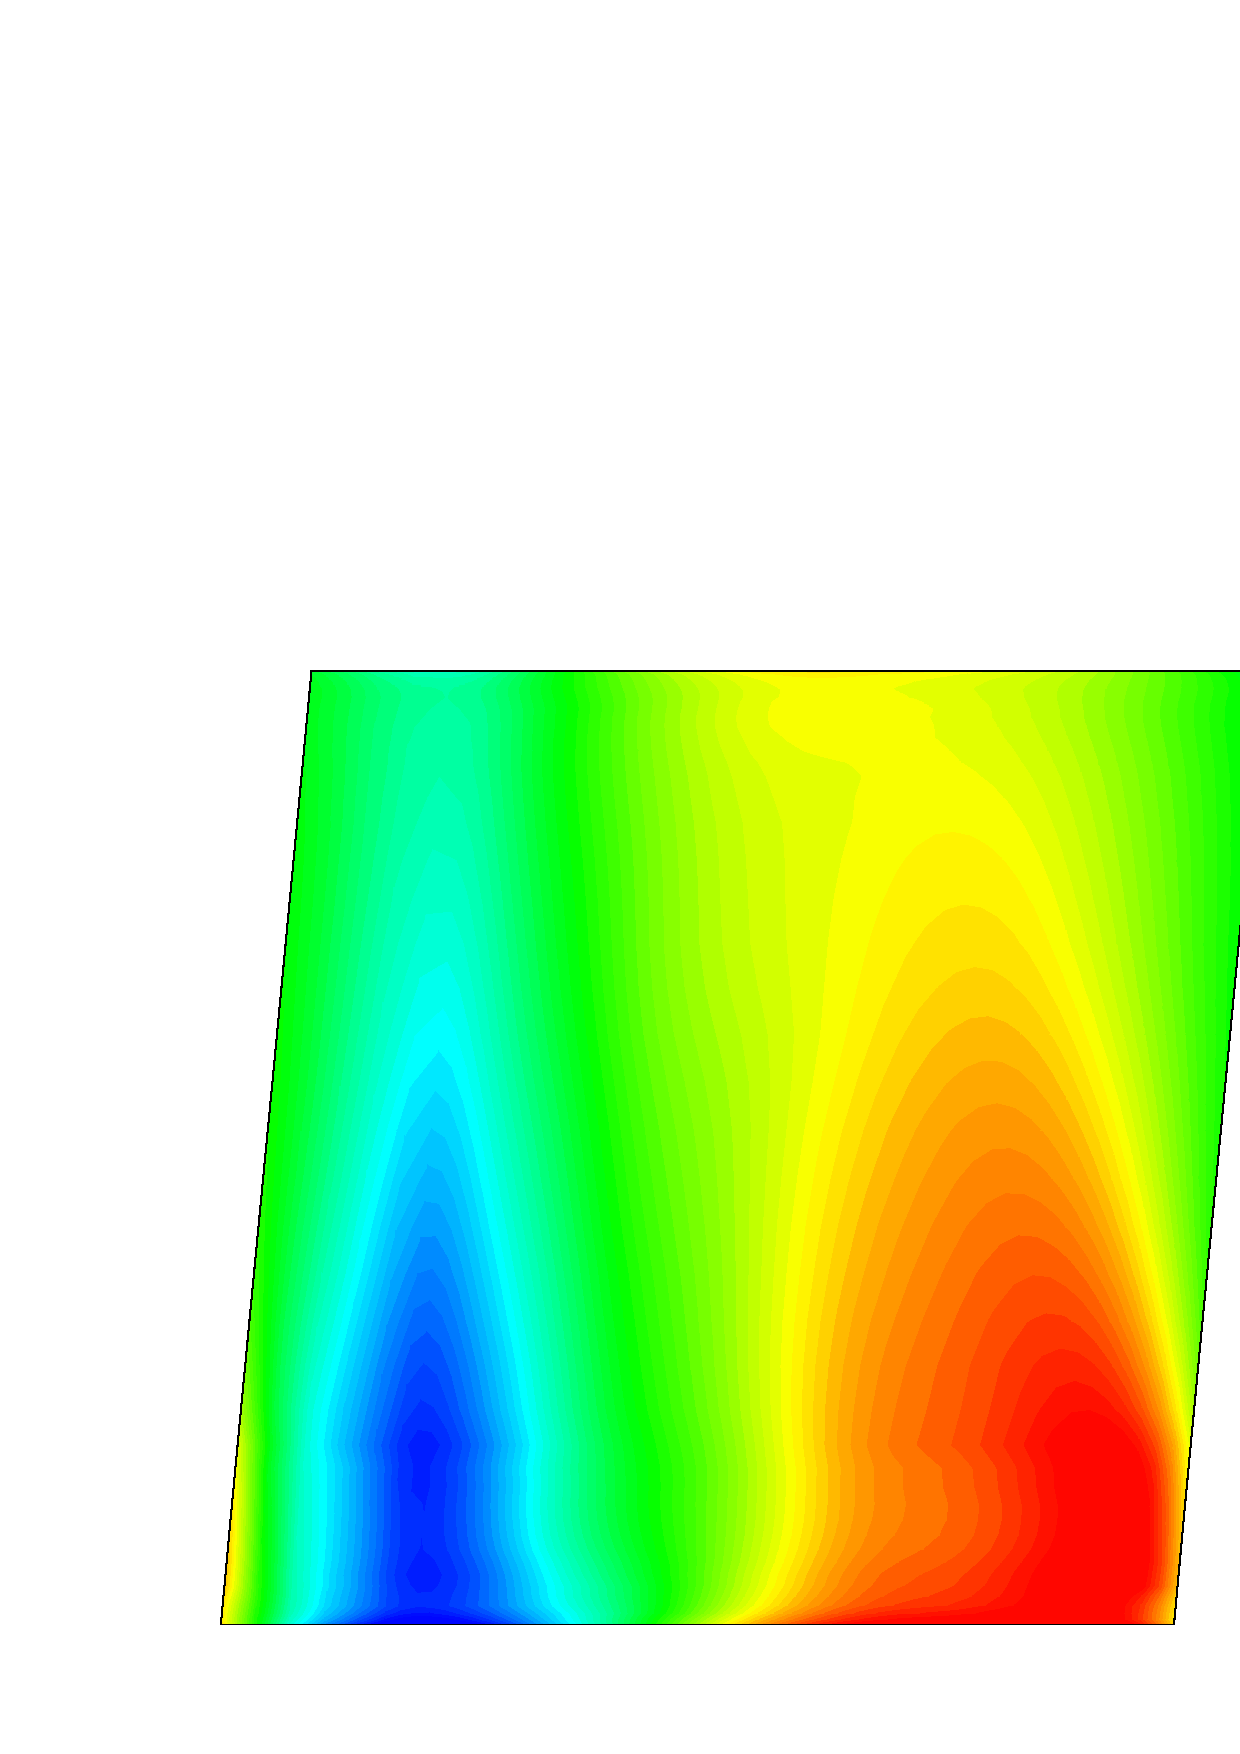
\includegraphics[width=70mm,clip=t]{CHAP_RT27/FIGURE/out_vel_pot.pdf}}
  \end{tabular}
 \end{center}
 \vspace{-8mm}
 \caption{Vortical and potential components of
          dimensionless absolute velocity variation at RT27a NGV outlet
          (reconstructed using first twenty harmonics)}
 \label{ngv_outlet_decomposed2.fig}
\end{figure}
%
 Fig. \ref{ngv_outlet_decomposed2.fig} shows the vortical and potential components
 of the absolute velocity non-uniformities at the NGV outlet. These two plots
 have been obtained by a summation of the first twenty
 vortical and potential Fourier components.
%
%
%
%
%
\subsection{Comparison with measured data}
\label{rt27_comparison.subsec}
%
 The computed unsteady flow results, obtained from the superimposition of
 the potential and vortical calculations, will
 now be compared with the experimental data of Moss et al. \citeyear{Moss:1}.
 The comparison is made for three different span-wise positions, namely
 mid-root, mid-height and tip. The remaining two sections, root
 and mid-tip, are not considered because of the unavailability of
 experimental data for the rotor suction surface.
%
%
\begin{figure}
  \begin{flushleft}
   \begin{tabular}{l}
     \subfigure[Mid-root section ($10\%$ span)]
      {\begin{tabular}{ll}
        \hspace{-5mm}
        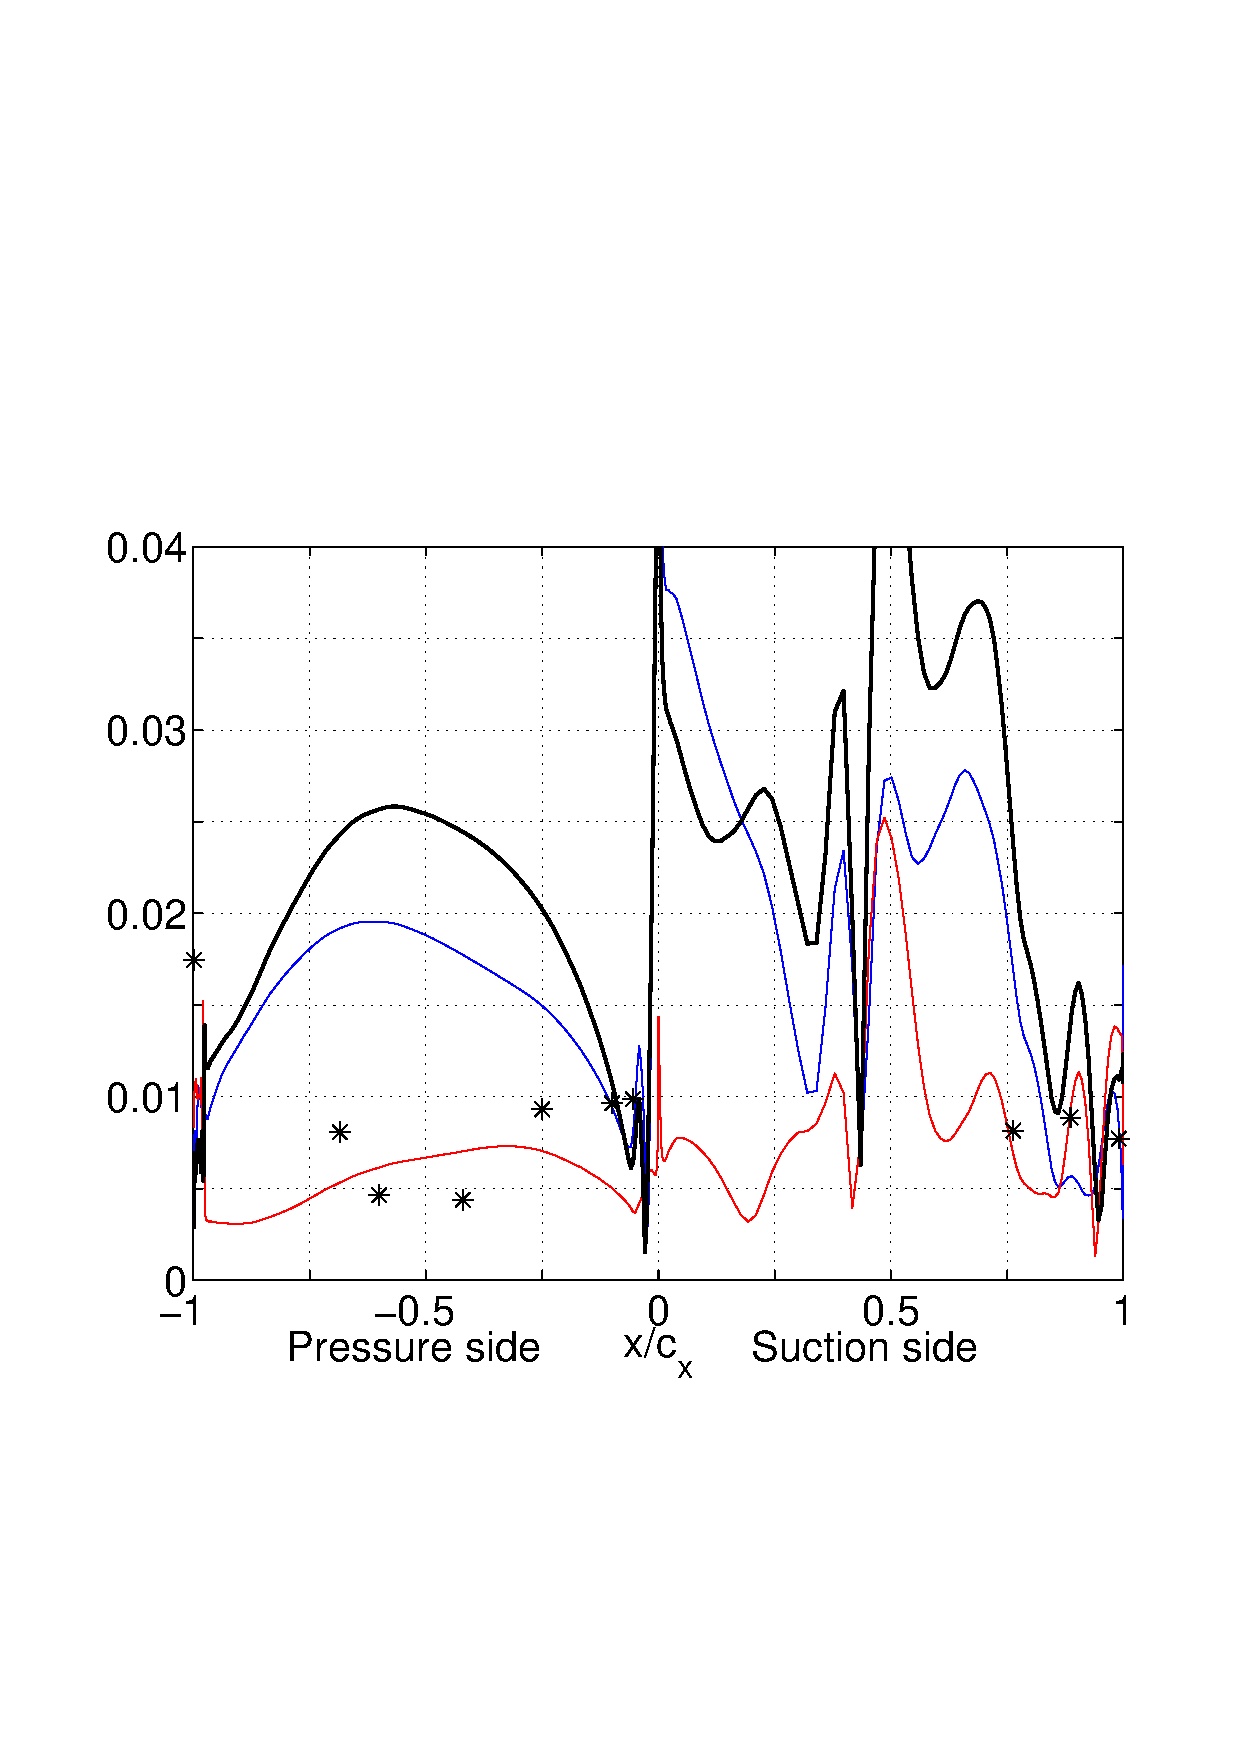
\includegraphics[width=70mm,clip=t]{CHAP_RT27/FIGURE/amps2m1.pdf}
         &
        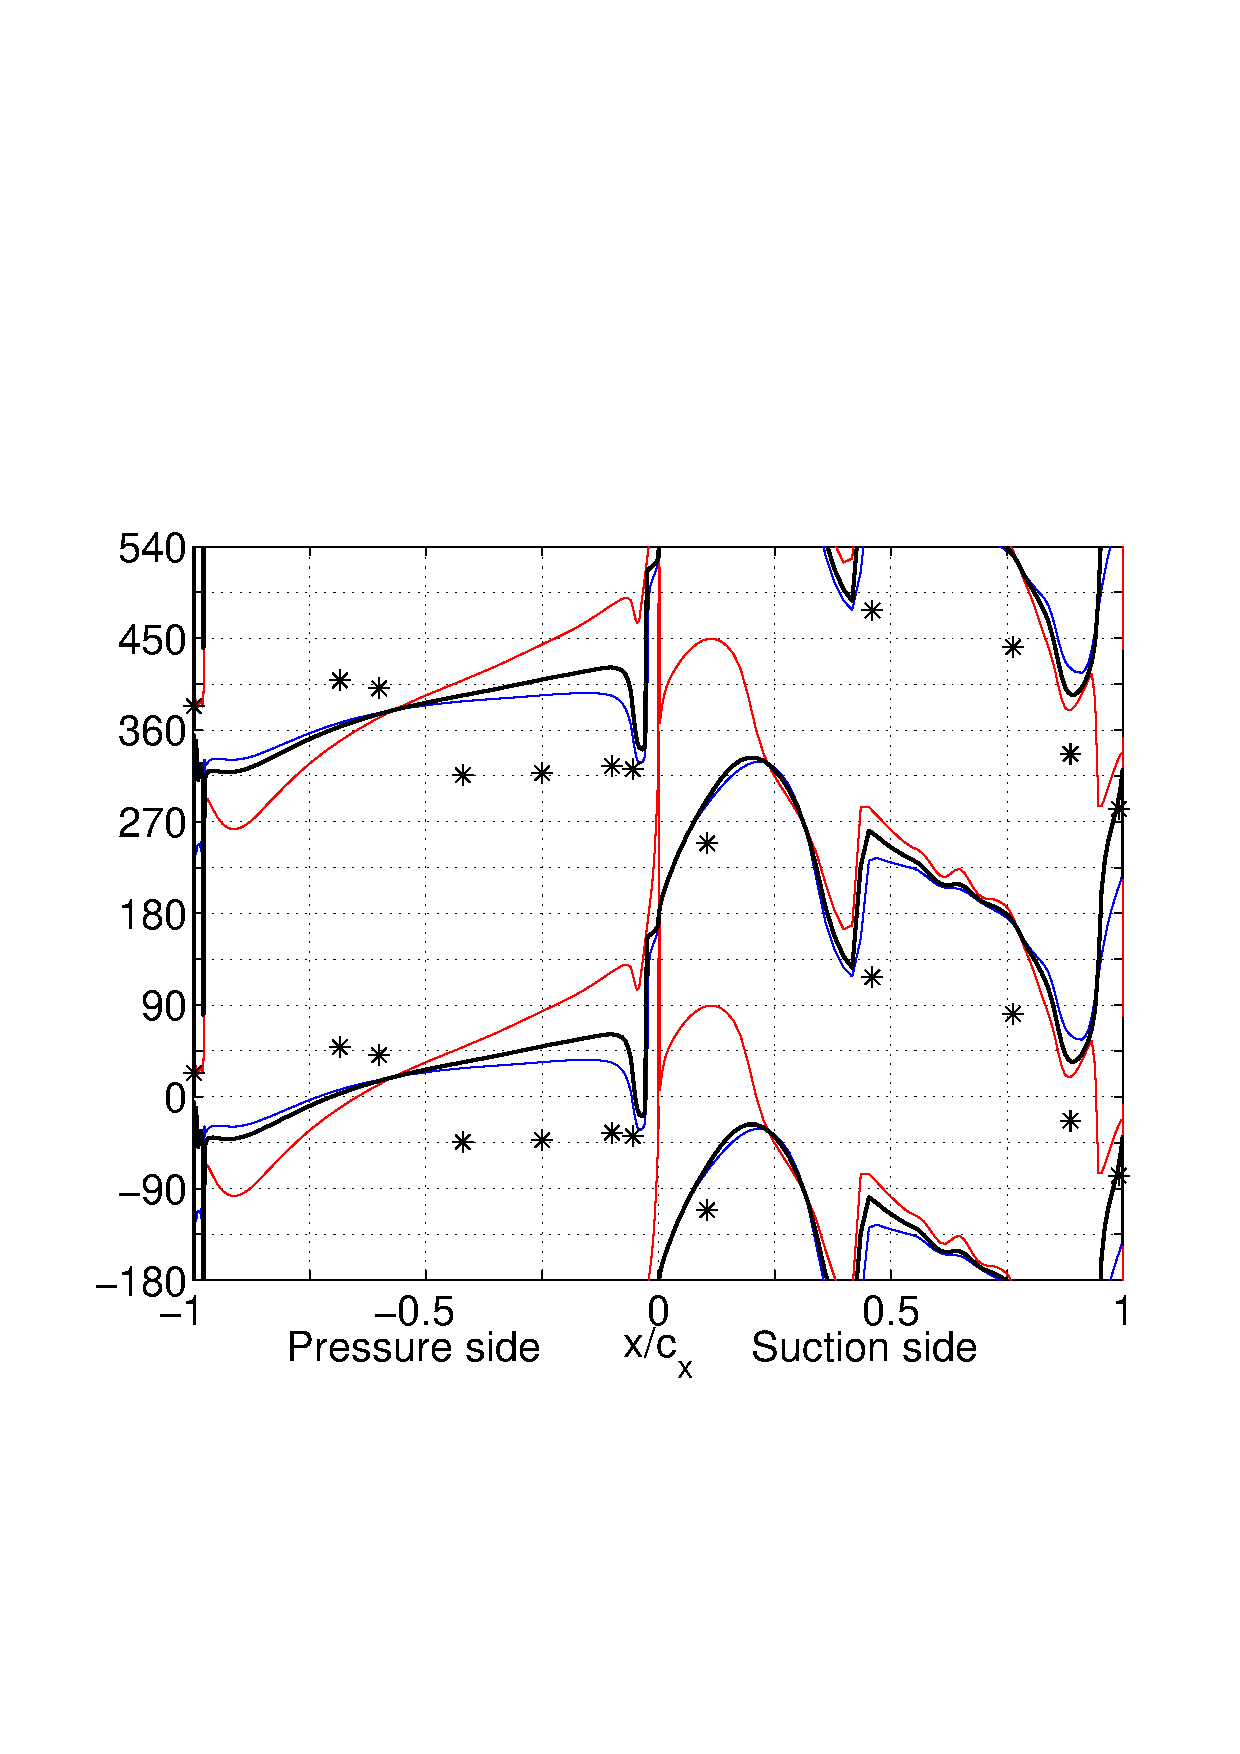
\includegraphics[width=70mm,clip=t]{CHAP_RT27/FIGURE/phas2m1.pdf}
       \end{tabular}}
      \vspace{-5mm}\\
     \subfigure[Mid-height section ($50\%$ span)]
      {\begin{tabular}{ll}
        \hspace{-5mm}
        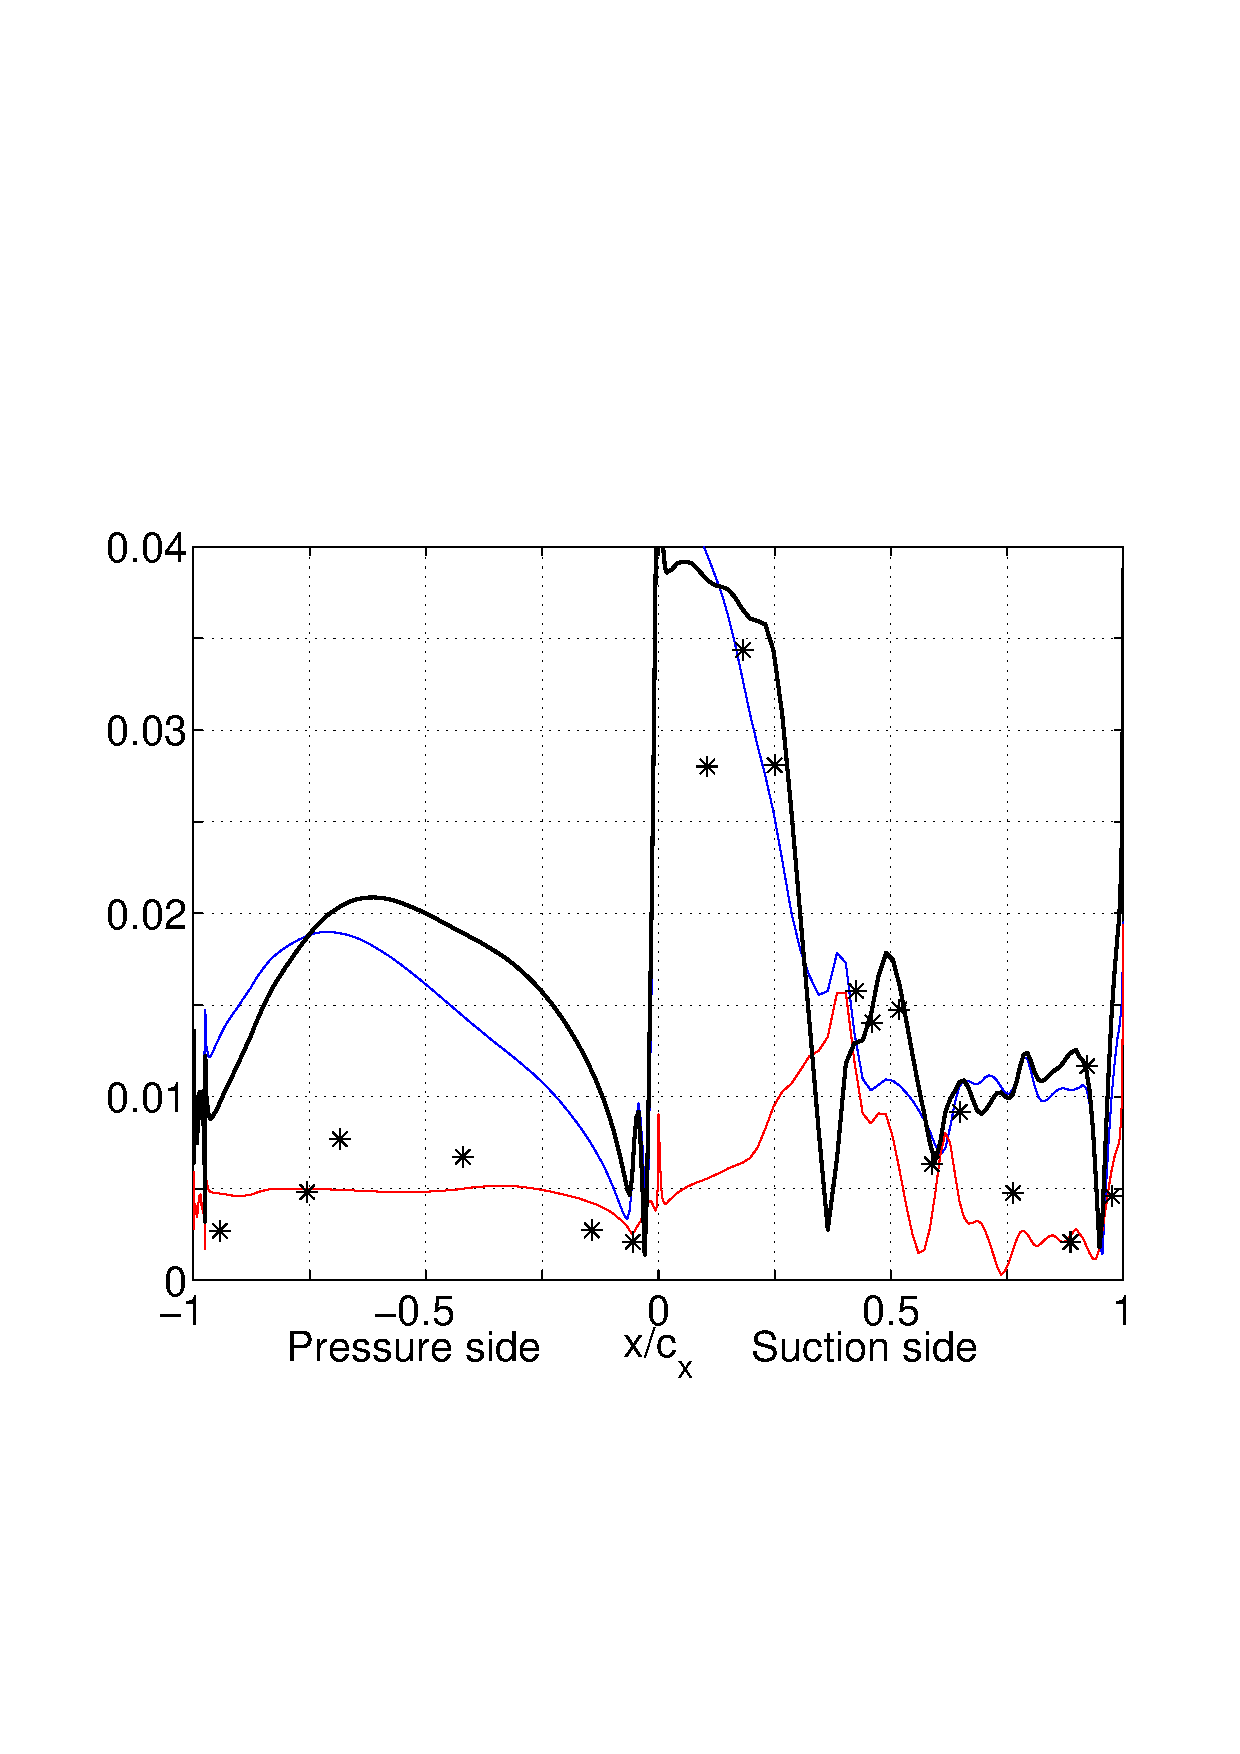
\includegraphics[width=70mm,clip=t]{CHAP_RT27/FIGURE/amps3m1.pdf}
         &
        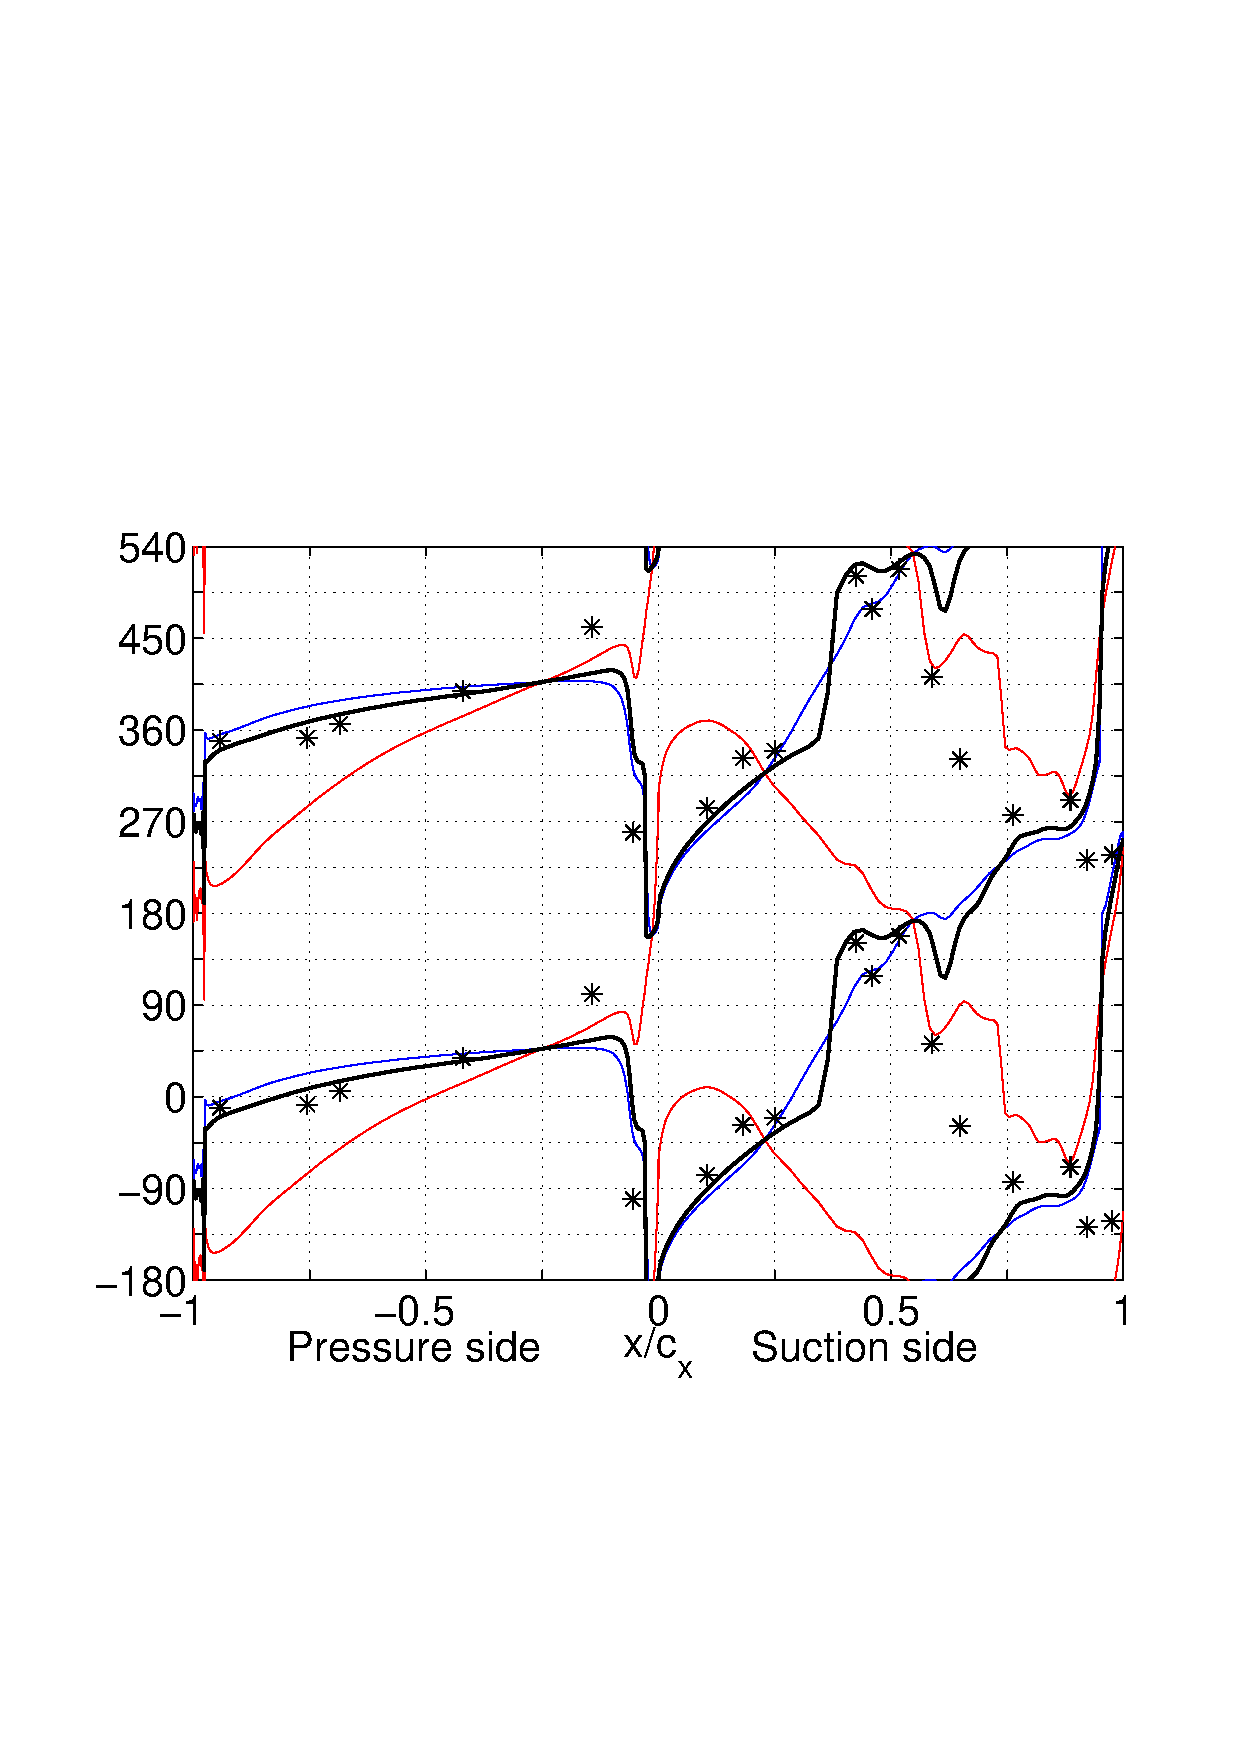
\includegraphics[width=70mm,clip=t]{CHAP_RT27/FIGURE/phas3m1.pdf}
       \end{tabular}}
      \vspace{-5mm}\\
     \subfigure[tip section ($95\%$ span)]
      {\begin{tabular}{ll}
        \hspace{-5mm}
        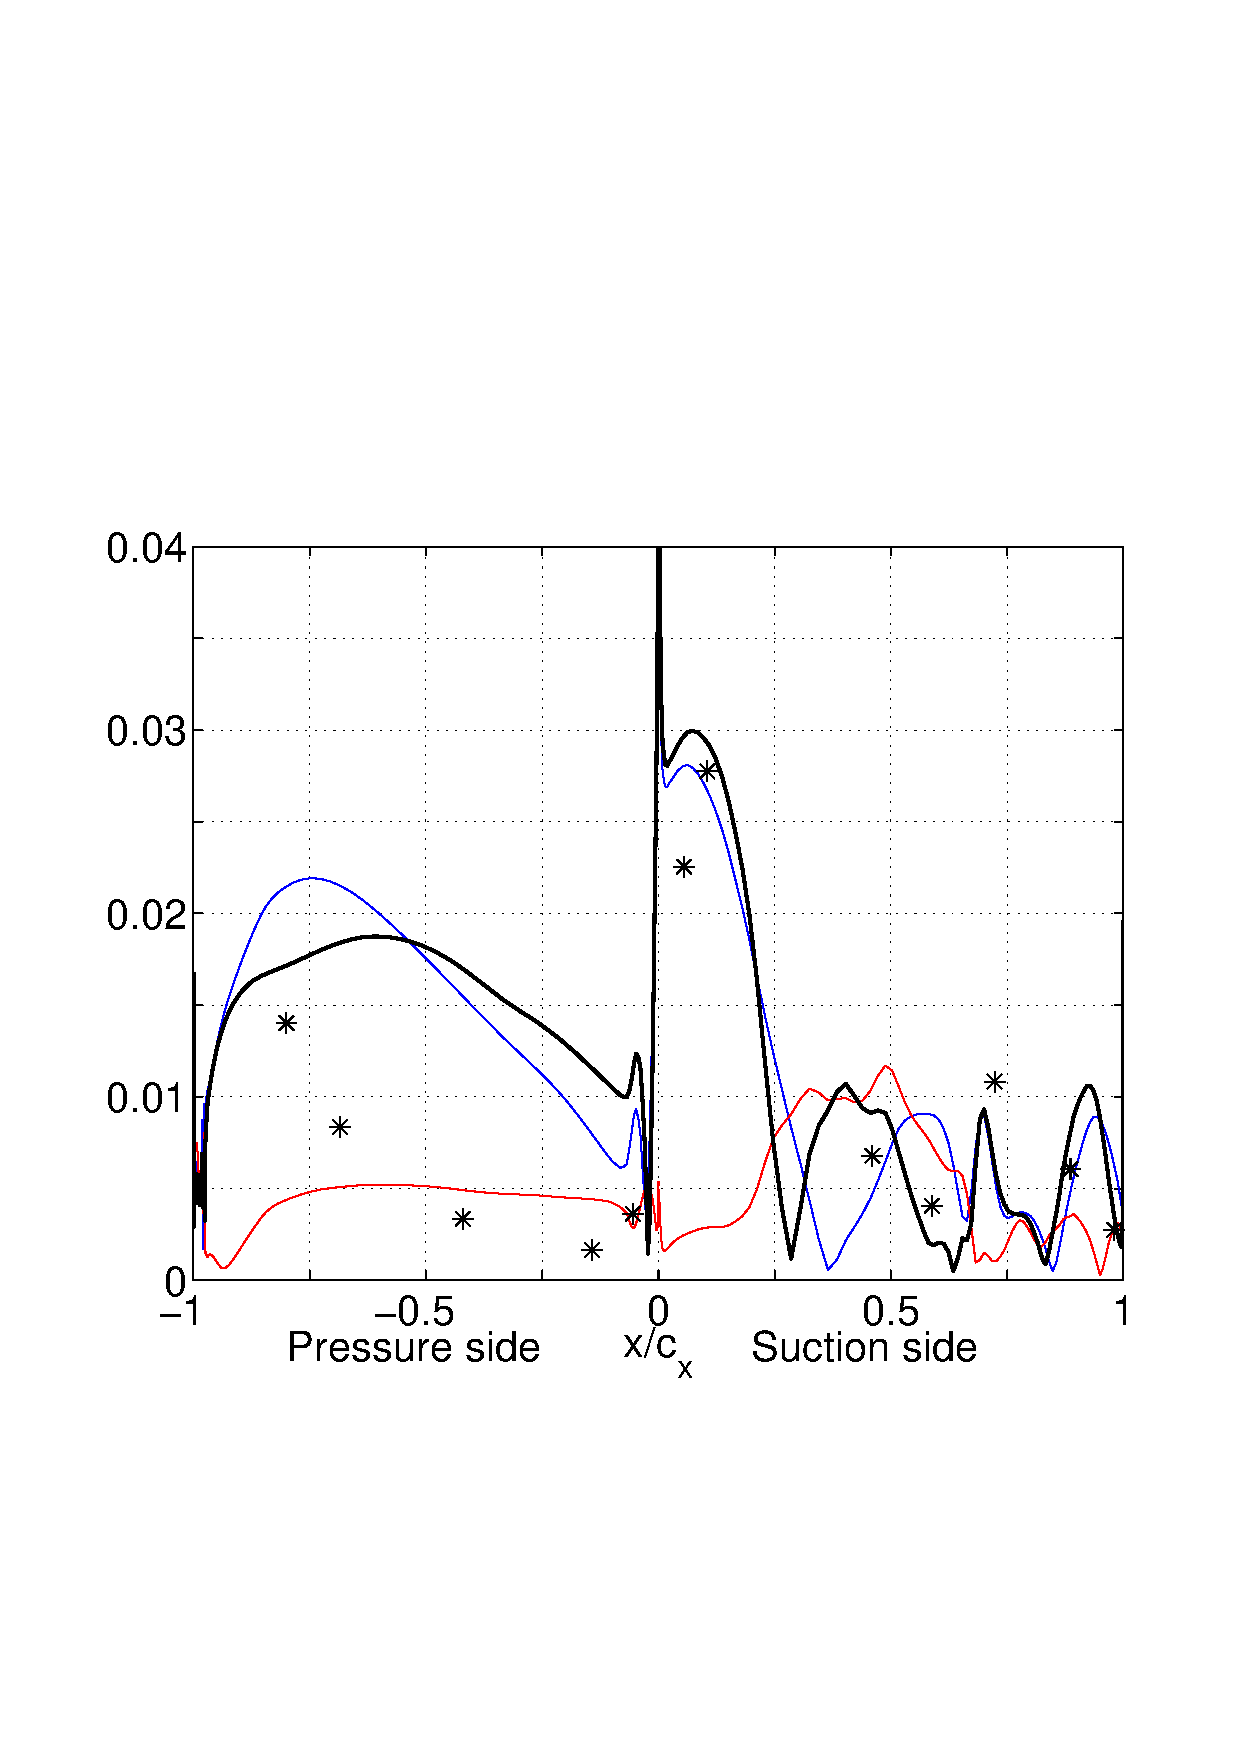
\includegraphics[width=70mm,clip=t]{CHAP_RT27/FIGURE/amps5m1.pdf}
         &
        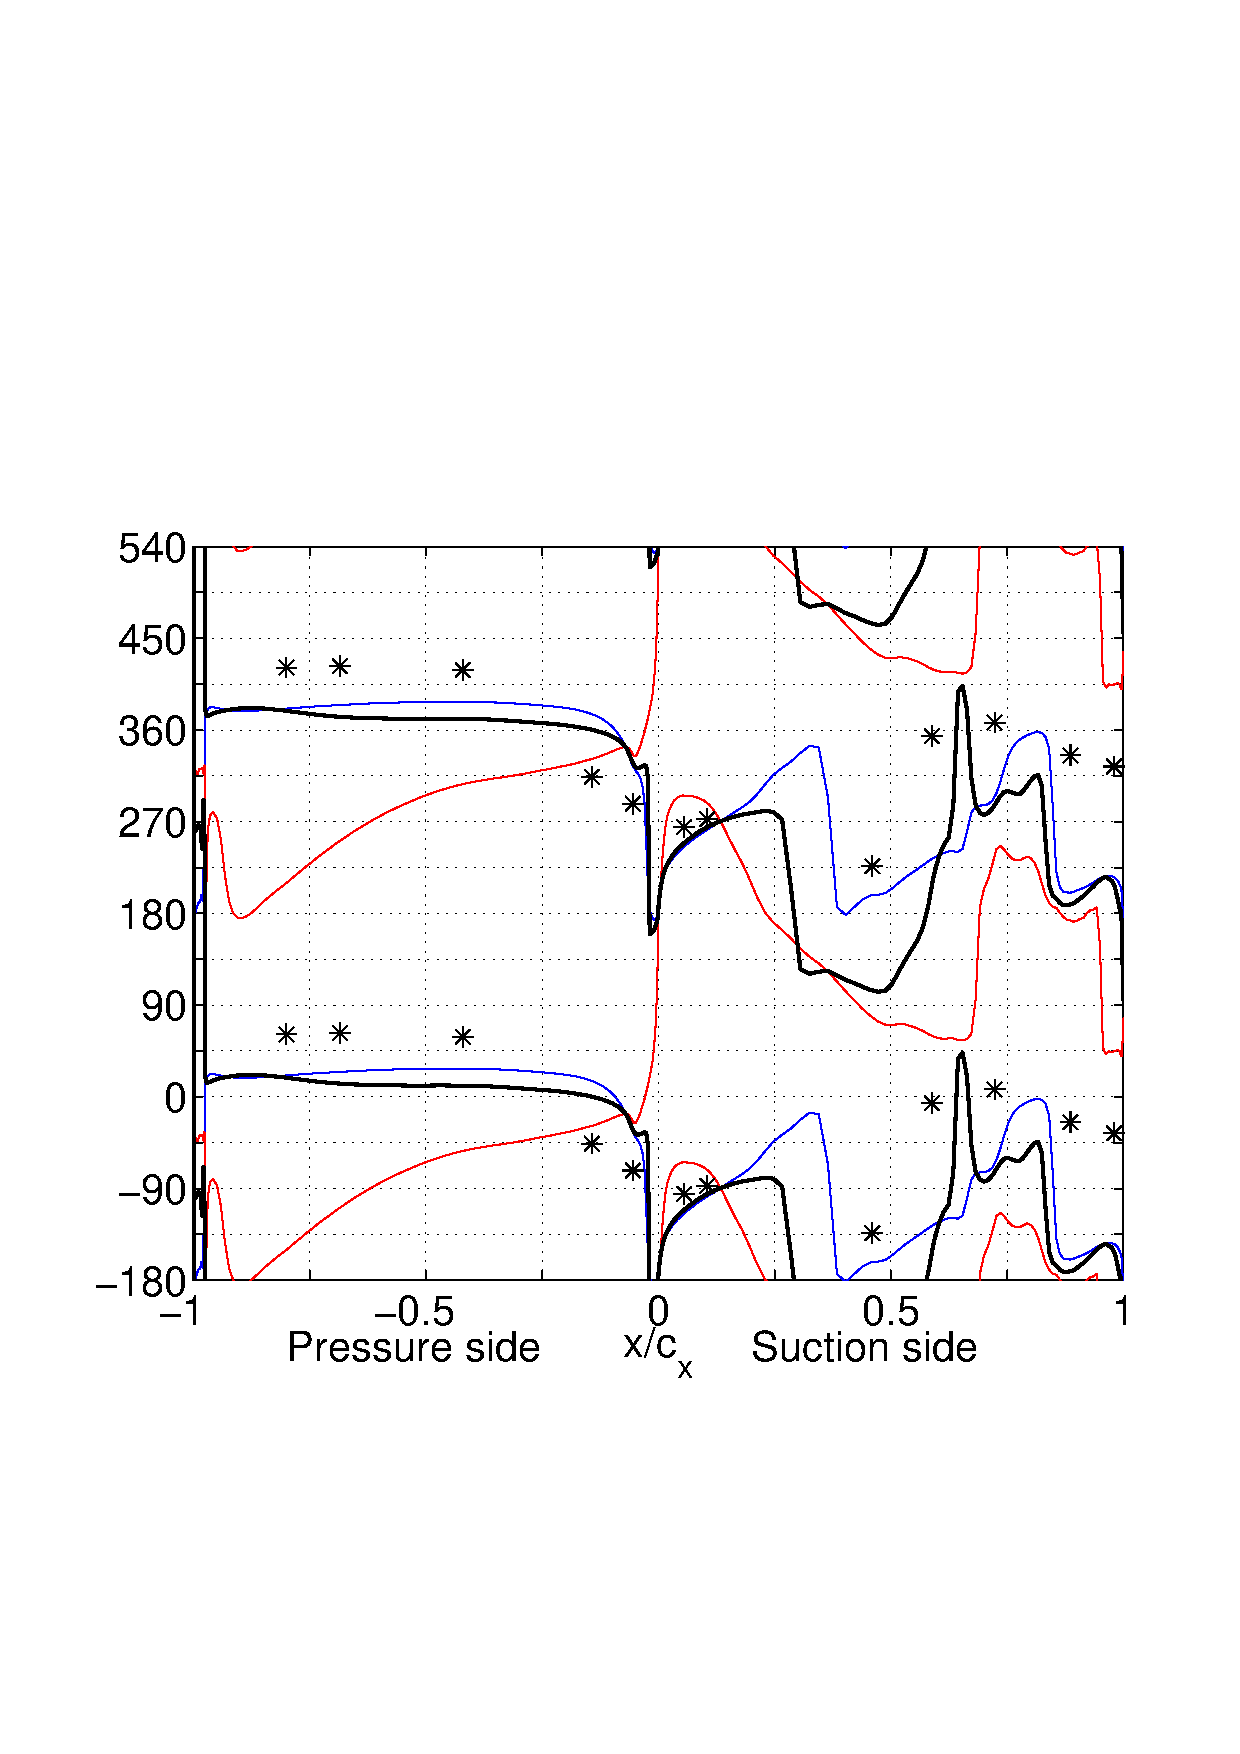
\includegraphics[width=70mm,clip=t]{CHAP_RT27/FIGURE/phas5m1.pdf}
       \end{tabular}}
   \end{tabular}
  \end{flushleft}
  \vspace{-8mm}
  \caption{Amplitude (left) and Phase (right) of
           first Fourier component of unsteady pressure $p/p_0$
           in the RT27a rotor blade.
           Potential mode (blue), vortical mode (red),
           superposed (black) and measured (*).}
  \label{rt27_unsteady3d_1.fig}
\end{figure}
%
%
 Fig. \ref{rt27_unsteady3d_1.fig} shows the amplitude and the
 phase angle of the first Fourier component of the unsteady pressure
 for these three radial sections.
 A striking feature of Fig. \ref{rt27_unsteady3d_1.fig} is that
 the pressure amplitude on the pressure surface is overpredicted
 for all three sections.
 This significant discrepancy is more evident in
 the mid-root section where shape of the predicted amplitude shows a maximum
 at mid-chord whereas the measured data indicate a minimum.
 On the other hand, at mid-height and tip, the shape of the predicted amplitude
 is similar to the measured ones even though there is a factor of two discrepancy.
 As it will be discussed in section \ref{linvnon_rt27.sec}, the reason of
 such discrepancy cannot be attributed to a possible
 non-linear behaviour.
%
%
\begin{figure}
  \begin{flushleft}
   \begin{tabular}{l}
     \subfigure[Mid-root section ($10\%$ span)]
      {\begin{tabular}{ll}
        \hspace{-5mm}
        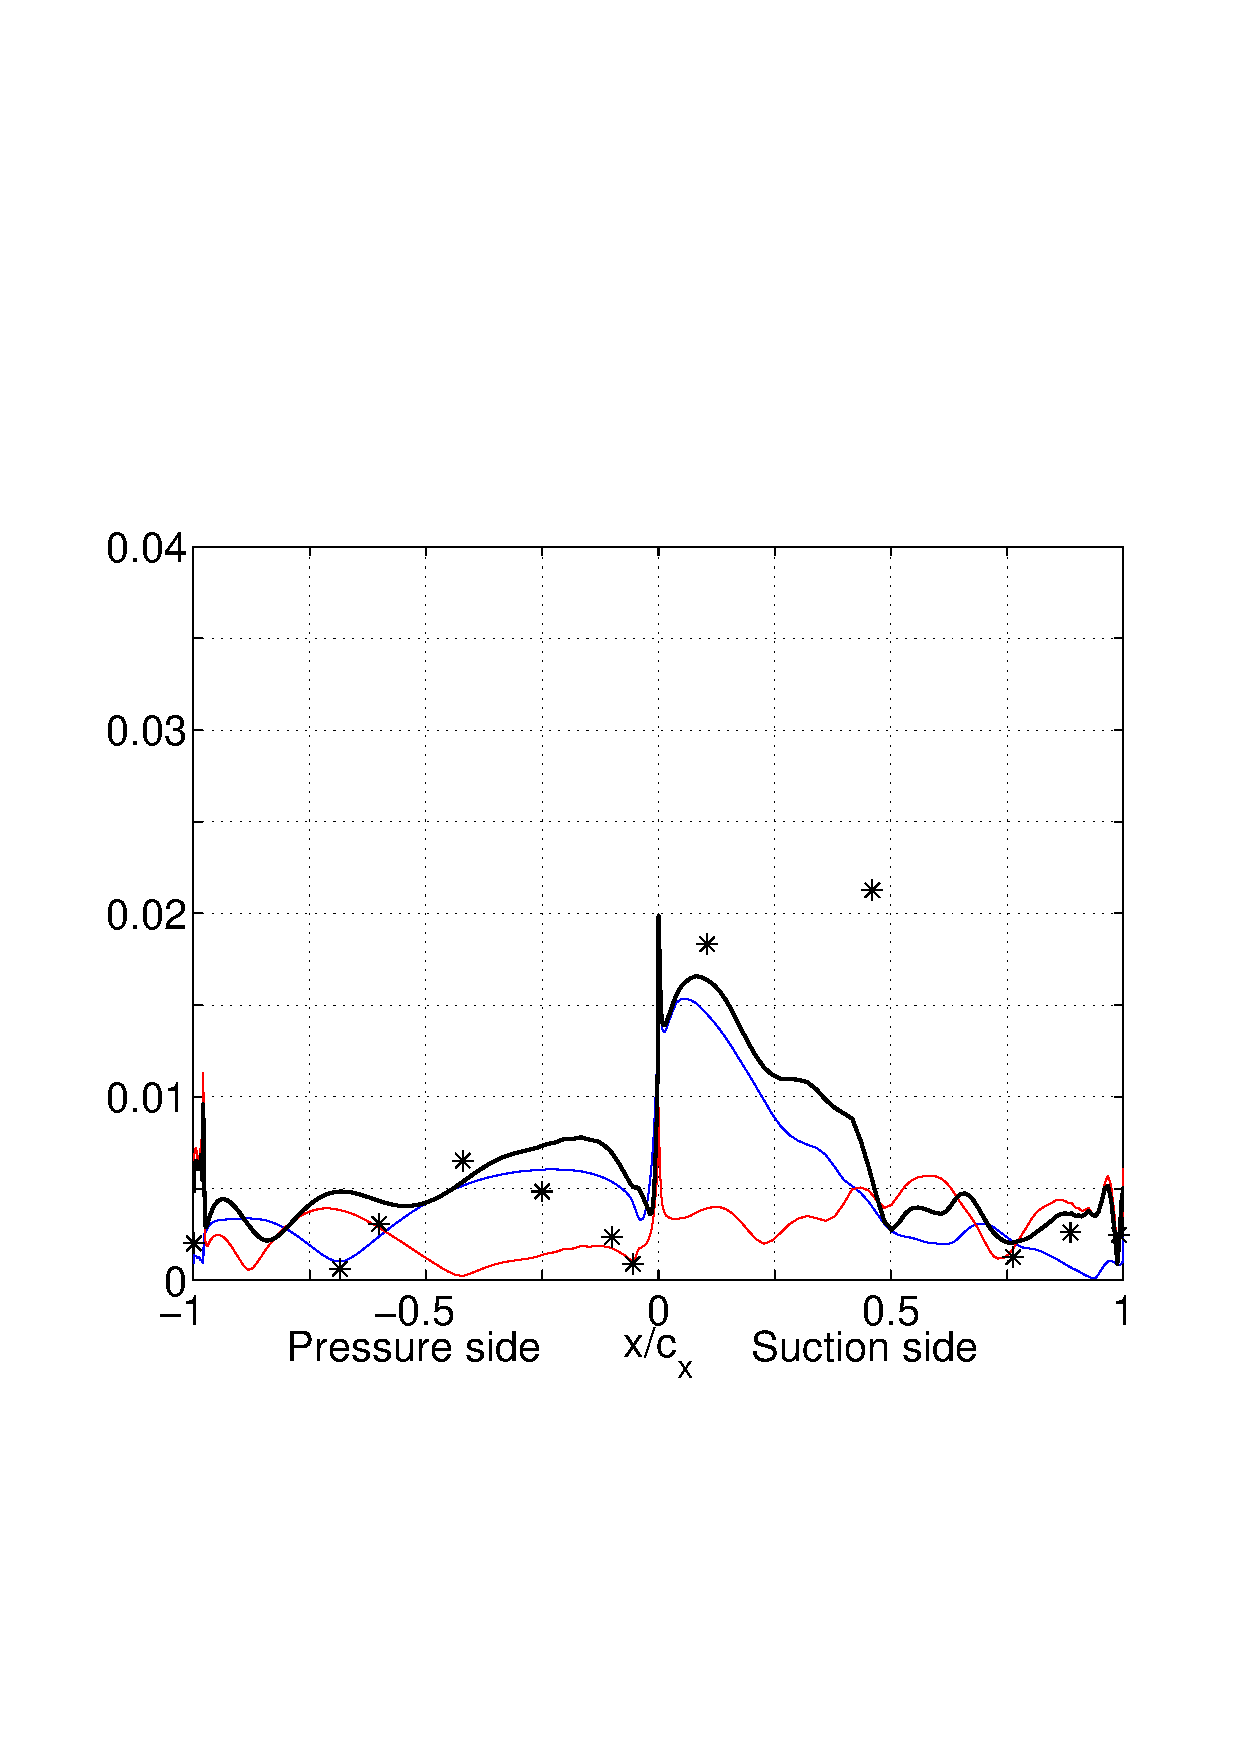
\includegraphics[width=70mm,clip=t]{CHAP_RT27/FIGURE/amps2m2.pdf}
         &
        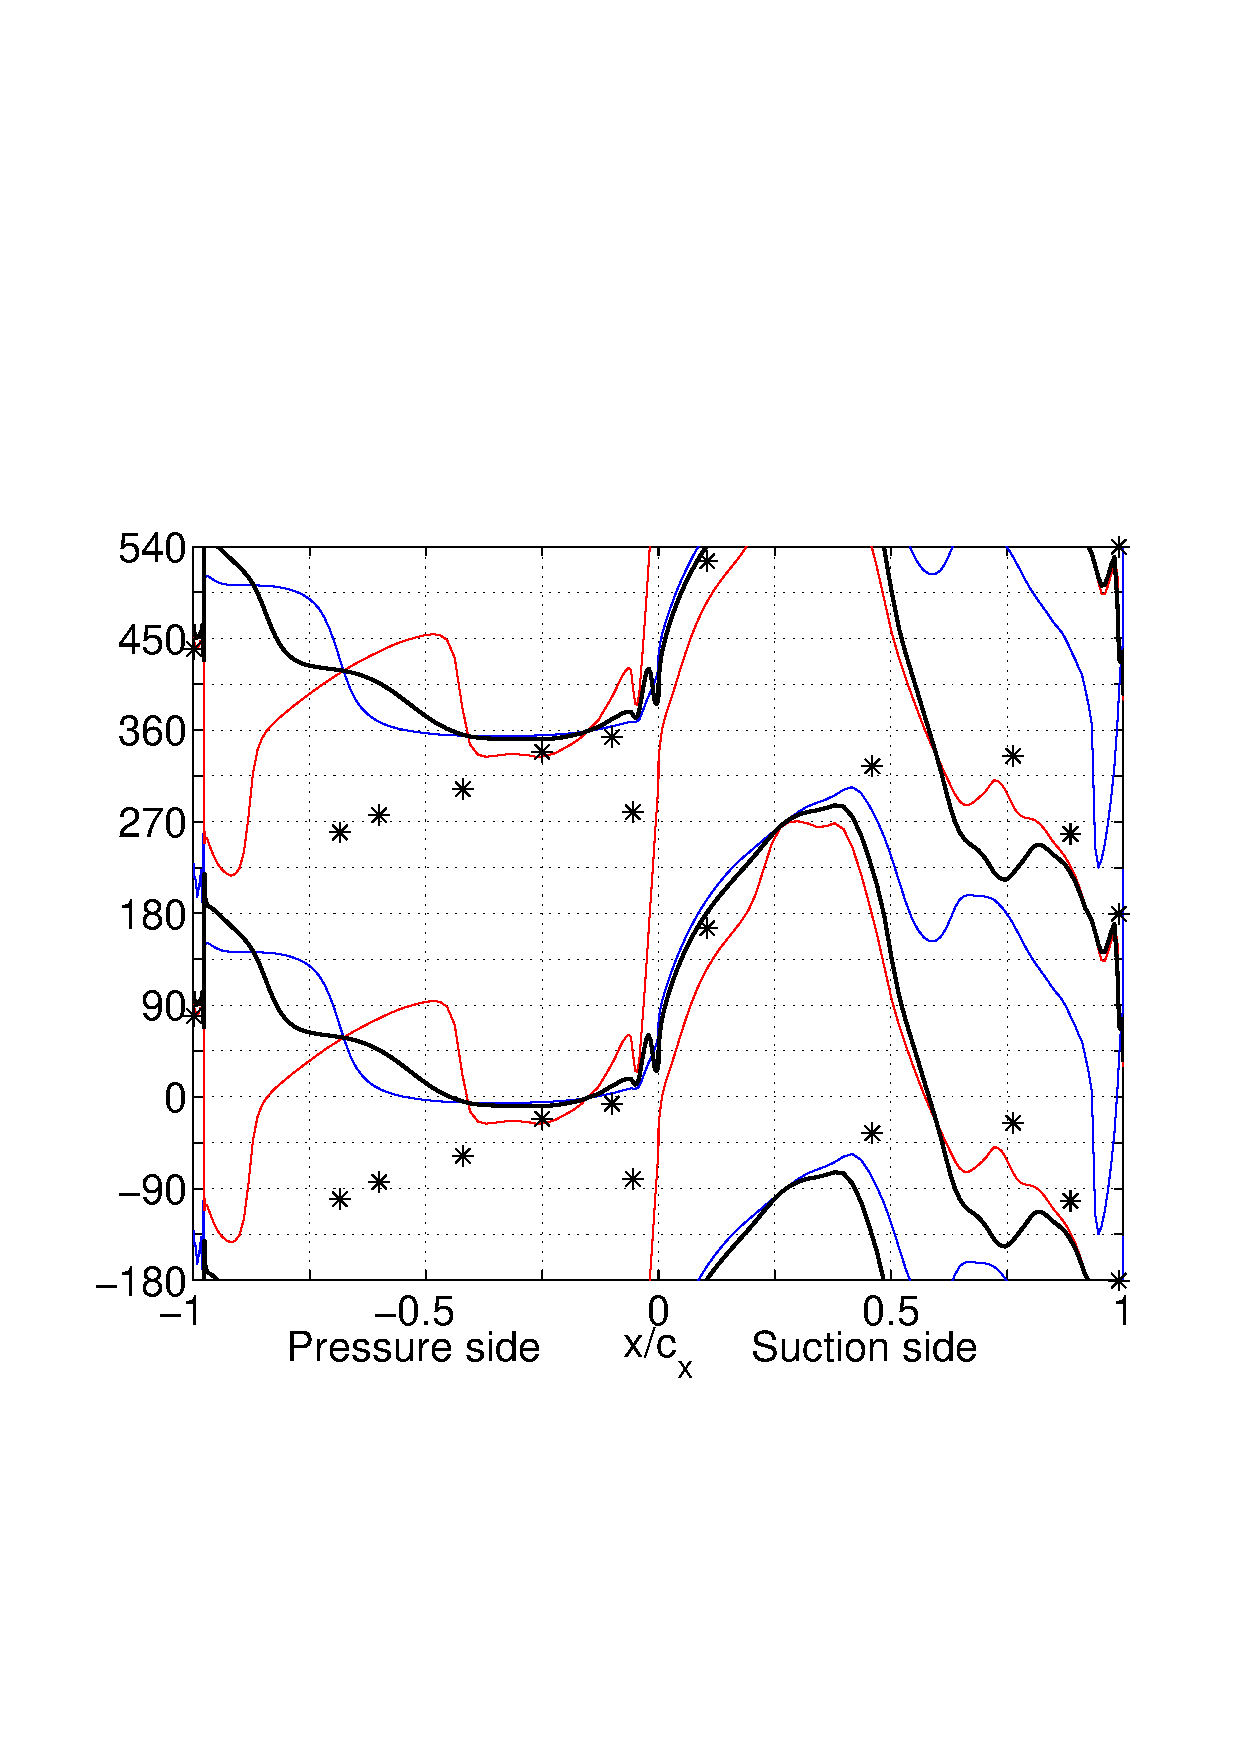
\includegraphics[width=70mm,clip=t]{CHAP_RT27/FIGURE/phas2m2.pdf}
       \end{tabular}}
      \vspace{-5mm}\\
     \subfigure[Mid-height section ($50\%$ span)]
      {\begin{tabular}{ll}
        \hspace{-5mm}
        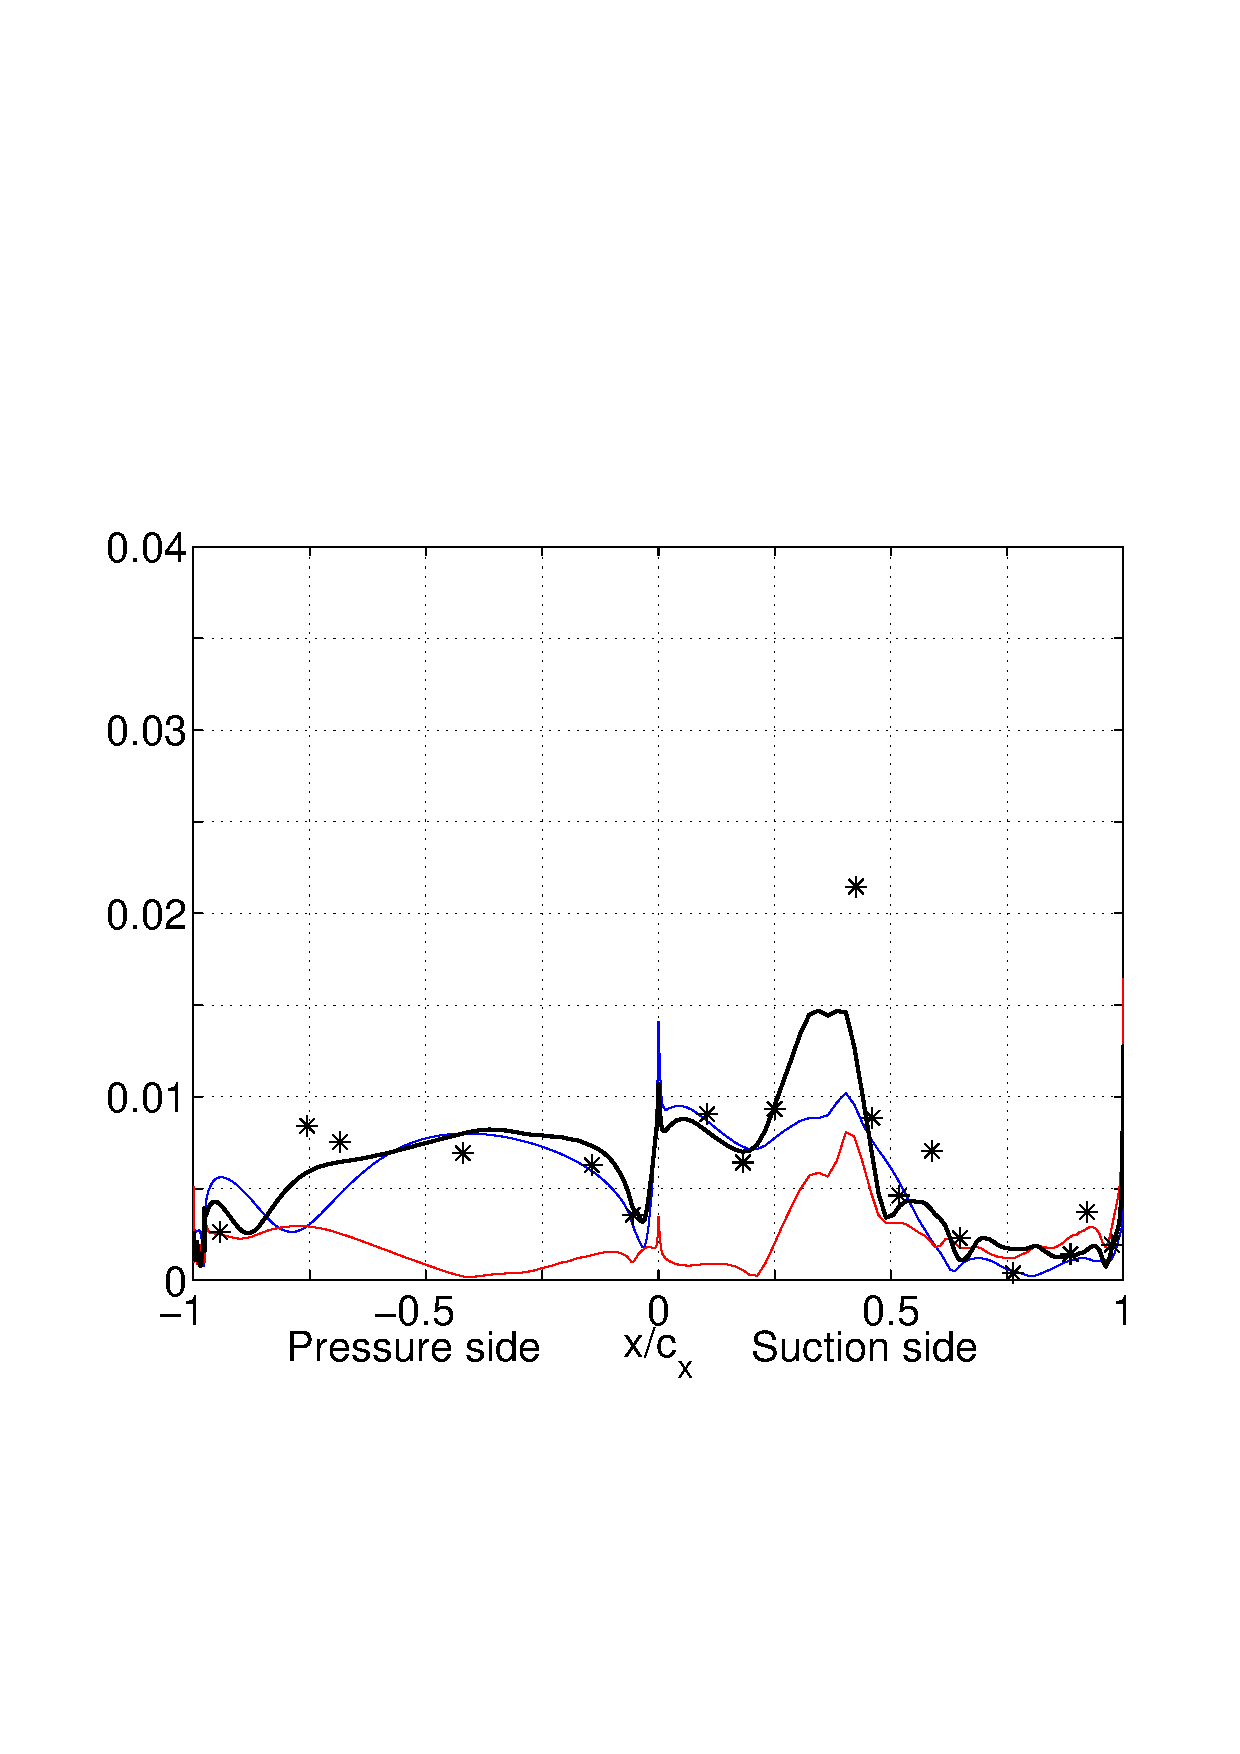
\includegraphics[width=70mm,clip=t]{CHAP_RT27/FIGURE/amps3m2.pdf}
         &
        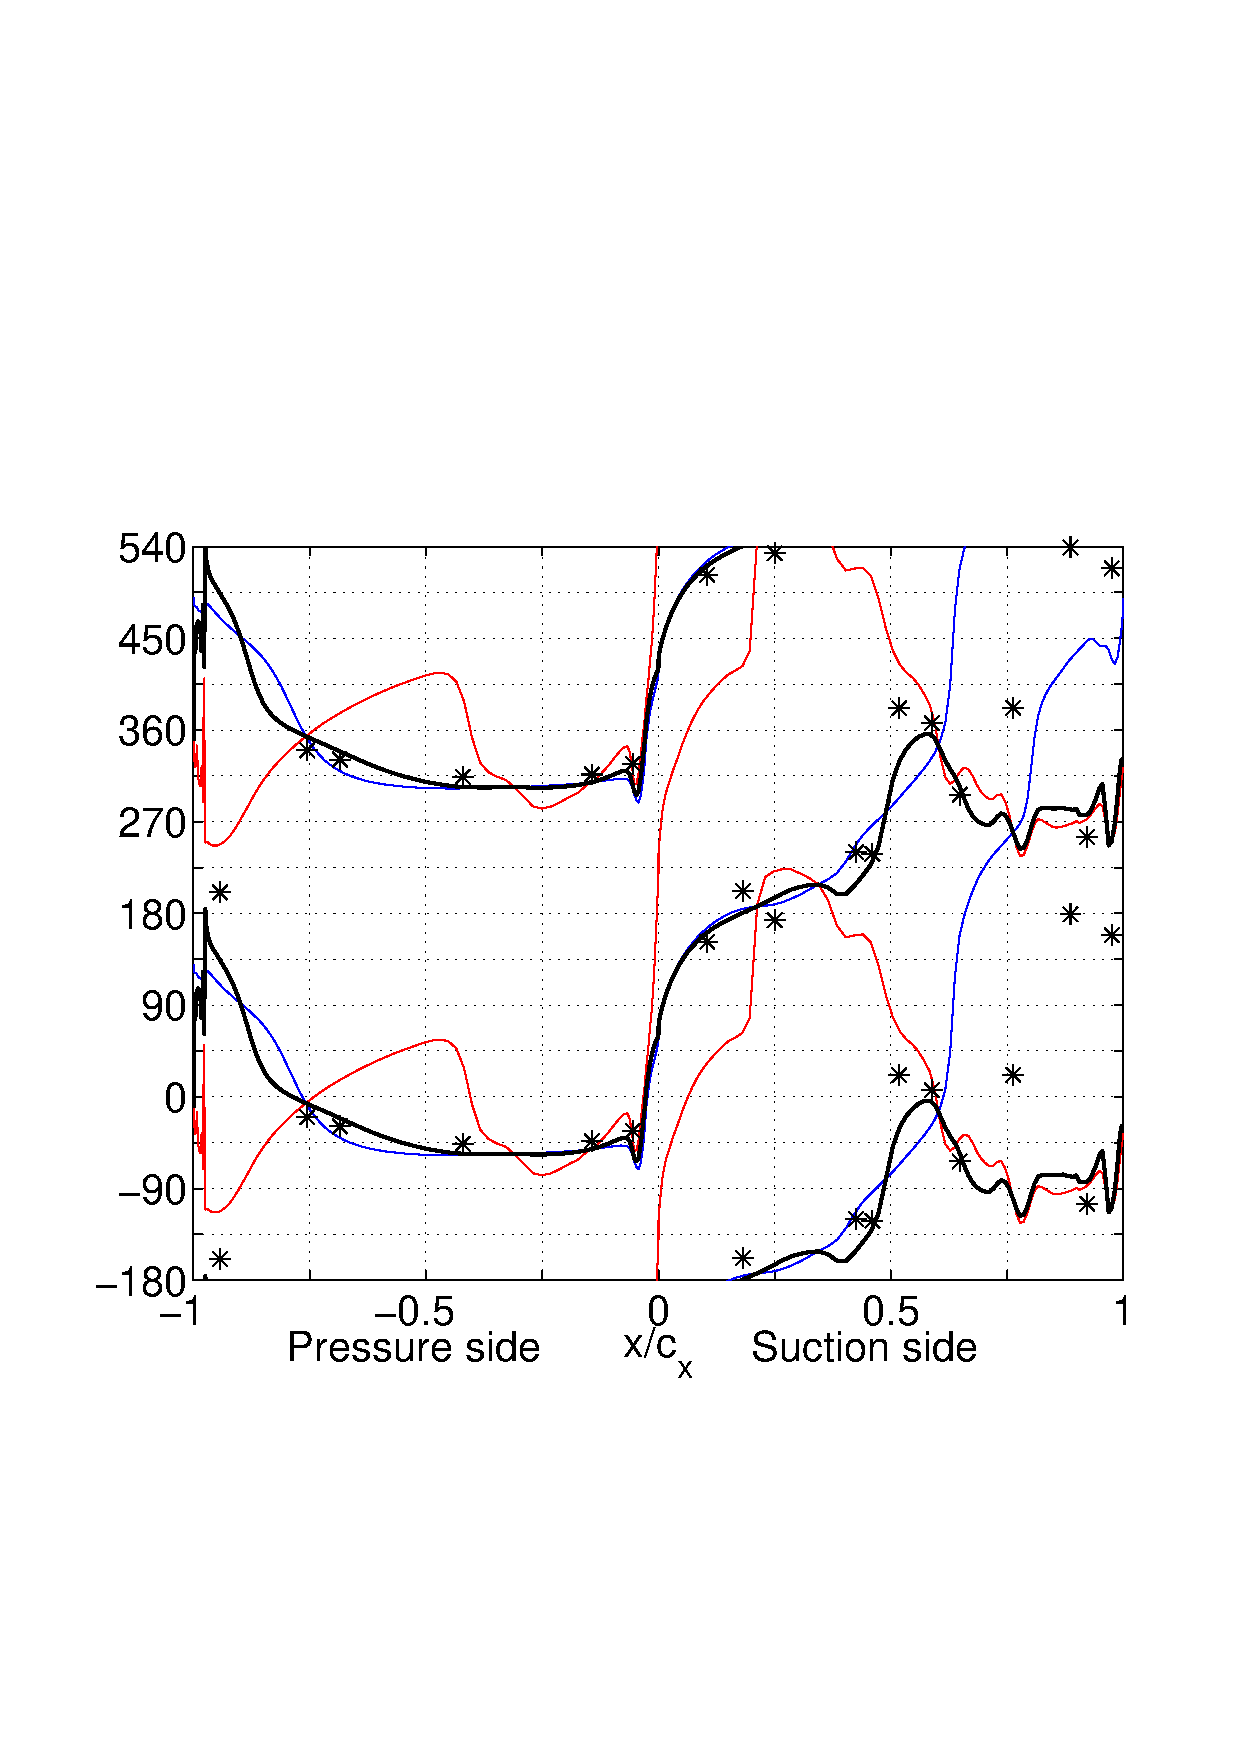
\includegraphics[width=70mm,clip=t]{CHAP_RT27/FIGURE/phas3m2.pdf}
       \end{tabular}}
      \vspace{-5mm}\\
     \subfigure[tip section ($95\%$ span)]
      {\begin{tabular}{ll}
        \hspace{-5mm}
        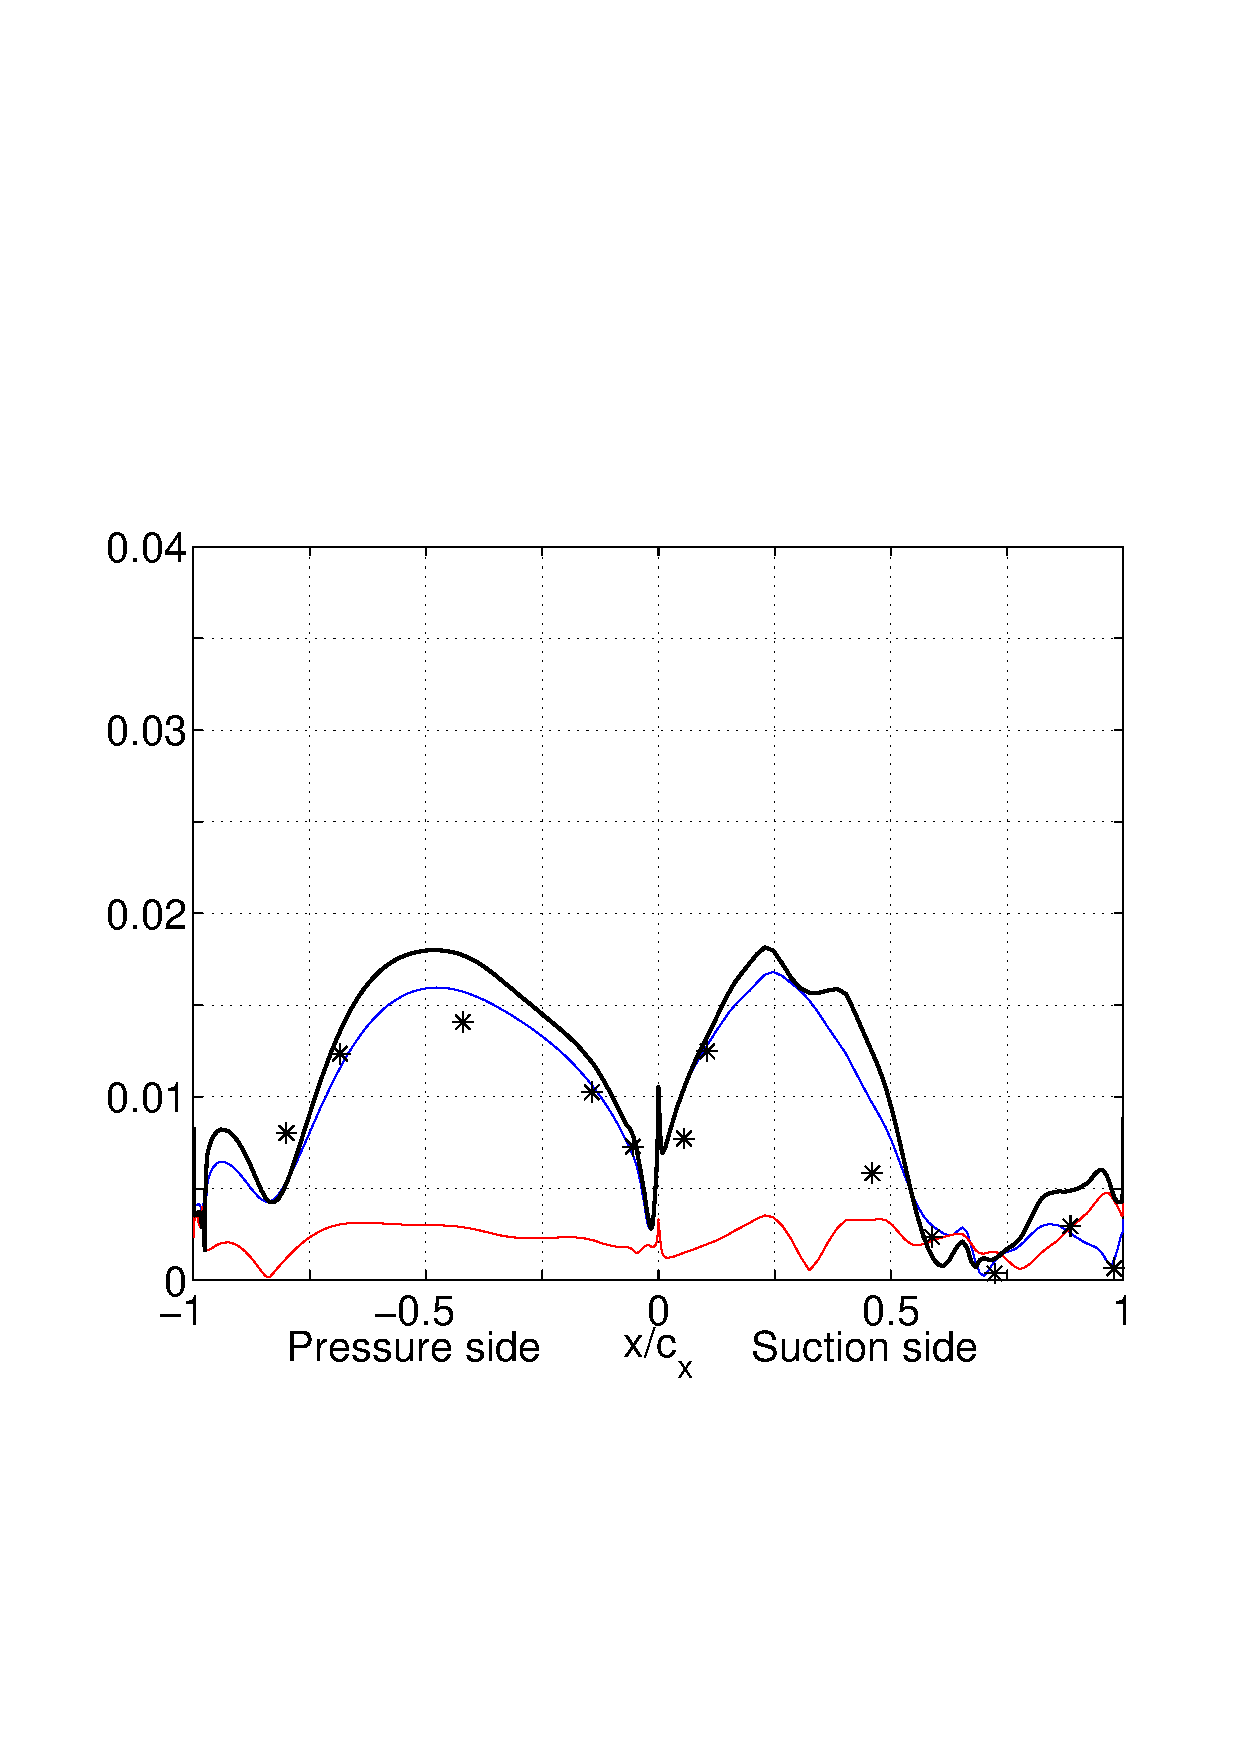
\includegraphics[width=70mm,clip=t]{CHAP_RT27/FIGURE/amps5m2.pdf}
         &
        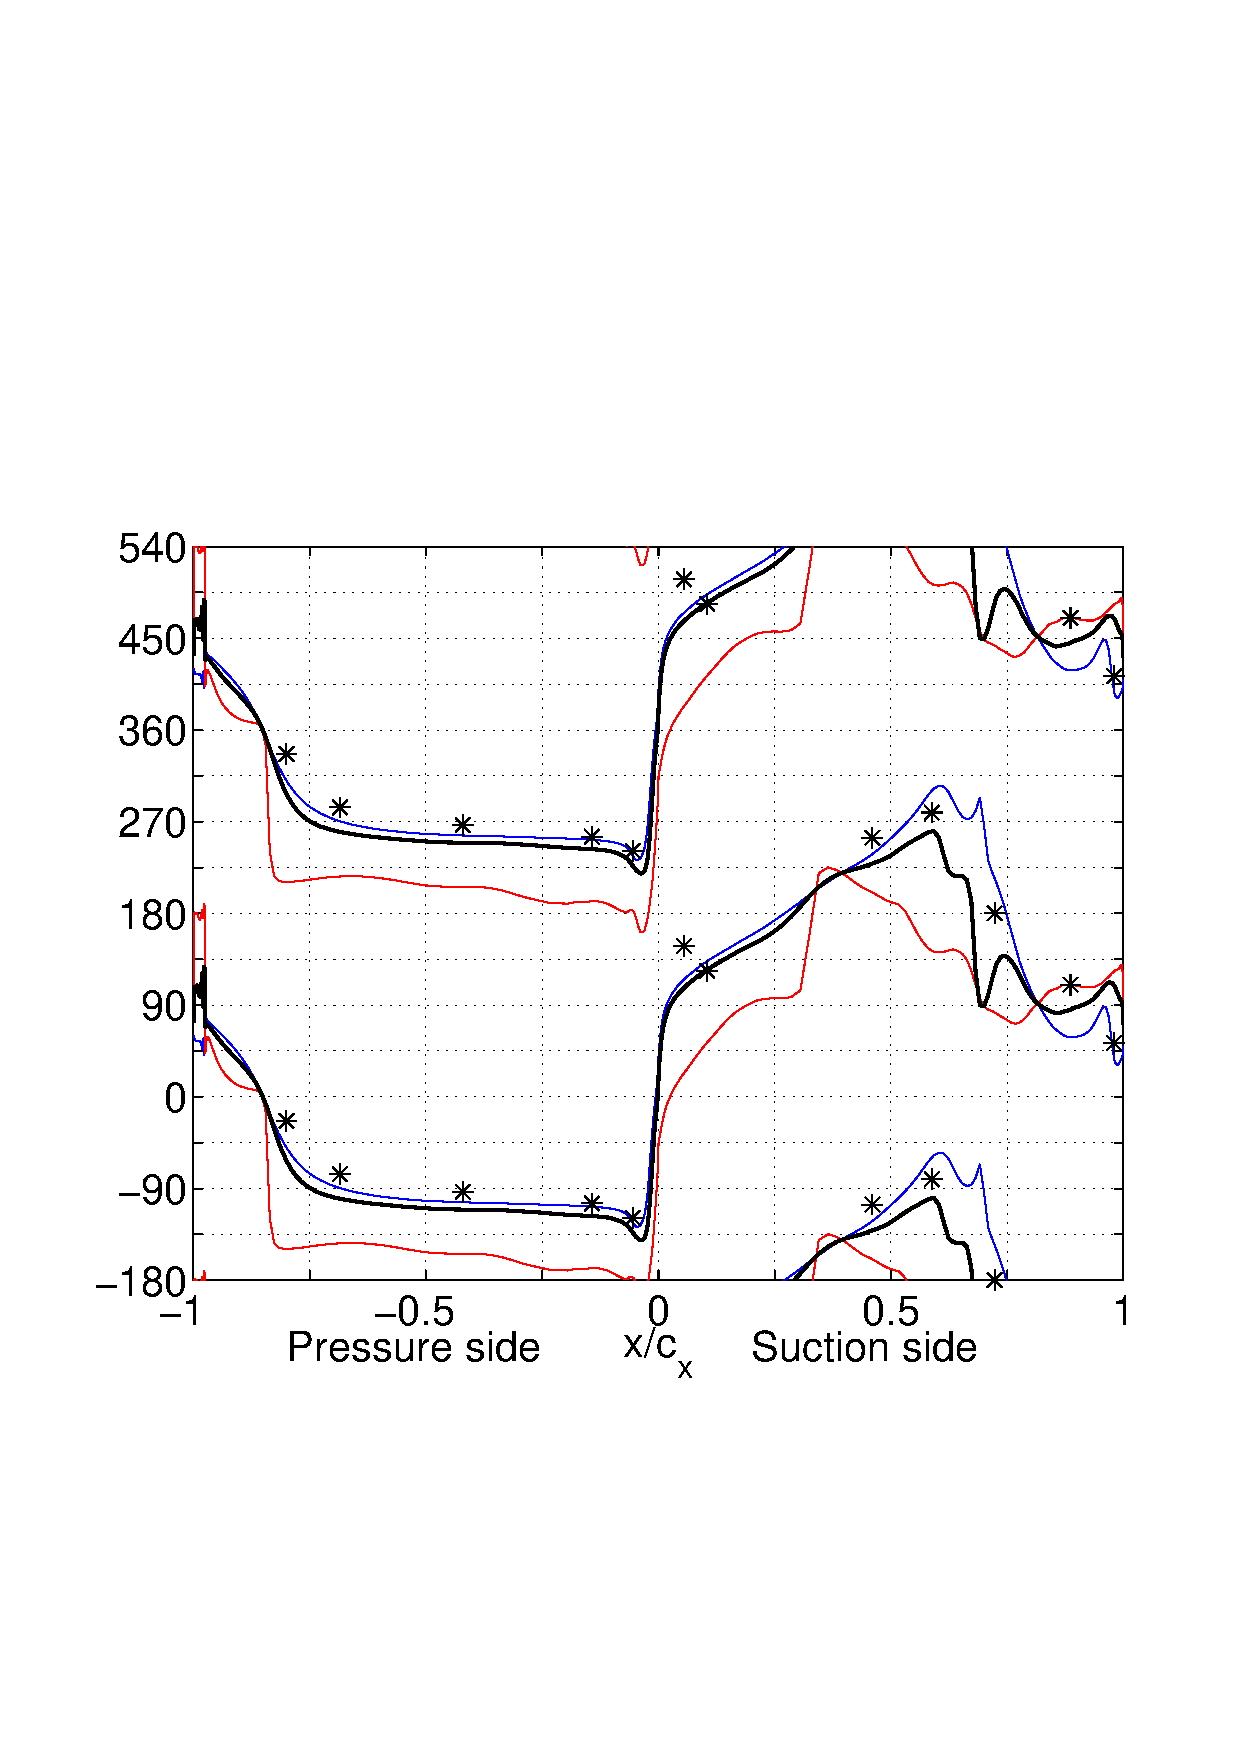
\includegraphics[width=70mm,clip=t]{CHAP_RT27/FIGURE/phas5m2.pdf}
       \end{tabular}}
   \end{tabular}
  \end{flushleft}
  \vspace{-8mm}
  \caption{Amplitude (left) and Phase (right) of
           second Fourier component of unsteady pressure $p/p_0$
           in the RT27a rotor blade.
           Potential mode (blue), vortical mode (red) and
           superposed (black), measured (stars).}
  \label{rt27_unsteady3d_2.fig}
\end{figure}
%
%
 Unlike the amplitude, the phase angle on the pressure side is in
 good agreement especially at mid-height and tip sections.
 The suction side predictions give a good representation,
 both in term of amplitude and phase angle. At mid-height, the suction side
 prediction has some discrepancies with the measured data in the region
 around $x/c\sm{x}\approx 0.75$ where the measured and computed data are out of
 phase and of different amplitudes.

~\newline
 Fig. \ref{rt27_unsteady3d_2.fig} shows the comparison between
 the predicted and measured data for the second Fourier component of the
 unsteady pressure.
 Unlikely the first Fourier component, and perhaps very surprisingly,
 the overall agreement is very good for the all three sections
 both in terms of amplitude and phase angle.
%
%
%
%
%
\subsection{Vortical-flow interaction effects}
\label{rt27_vortical.subsec}
%
 As discussed earlier the vortical flow non-uniformities
 at the NGV outlet are associated with a rotational
 velocity perturbation with zero divergence.
 Such a vortical flow component at the NGV outlet is shown in
 Fig. \ref{ngv_outlet_decomposed1.fig}a for the first two
 tangential Fourier modes.
 Vortical-flow interaction, also labelled wake-rotor interaction,
 has been studied and interpreted by several authors
 (Hodson \citeyearNP{Hodson:1}, Giles \citeyearNP{Giles:2},
 Korakianitis \citeyearNP{Kora:1}, \citeyearNP{Kora:2},
 \citeyearNP{Kora:3}) and it is now fairly well understood.
 Before analysing the hub-to-tip distribution
 of the pressure amplitude, a brief description of the wake-rotor
 interaction at mid-height section is given.

~\newline
 Figs. \ref{rt27_vortical2d_1.fig} and \ref{rt27_vortical2d_2.fig}
 show the dimensionless absolute velocity and pressure fluctuations
 together with the unsteady particle traces during one blade passing
 cycle in the rotor passage.
 The wakes are first bent by the potential flow field of the rotor
 as shown in Fig. \ref{rt27_vortical2d_1.fig}a.
 When the leading-edge in the rotor stagnation region interacts with
 the lower momentum fluid in the wake, unsteady, recirculating flow
 patterns are established as shown in Fig. \ref{rt27_vortical2d_1.fig}a.
%
\begin{figure}
  \begin{center}
   \begin{tabular}{c}
     \subfigure[t = 0]
       {\hspace{-5mm}
        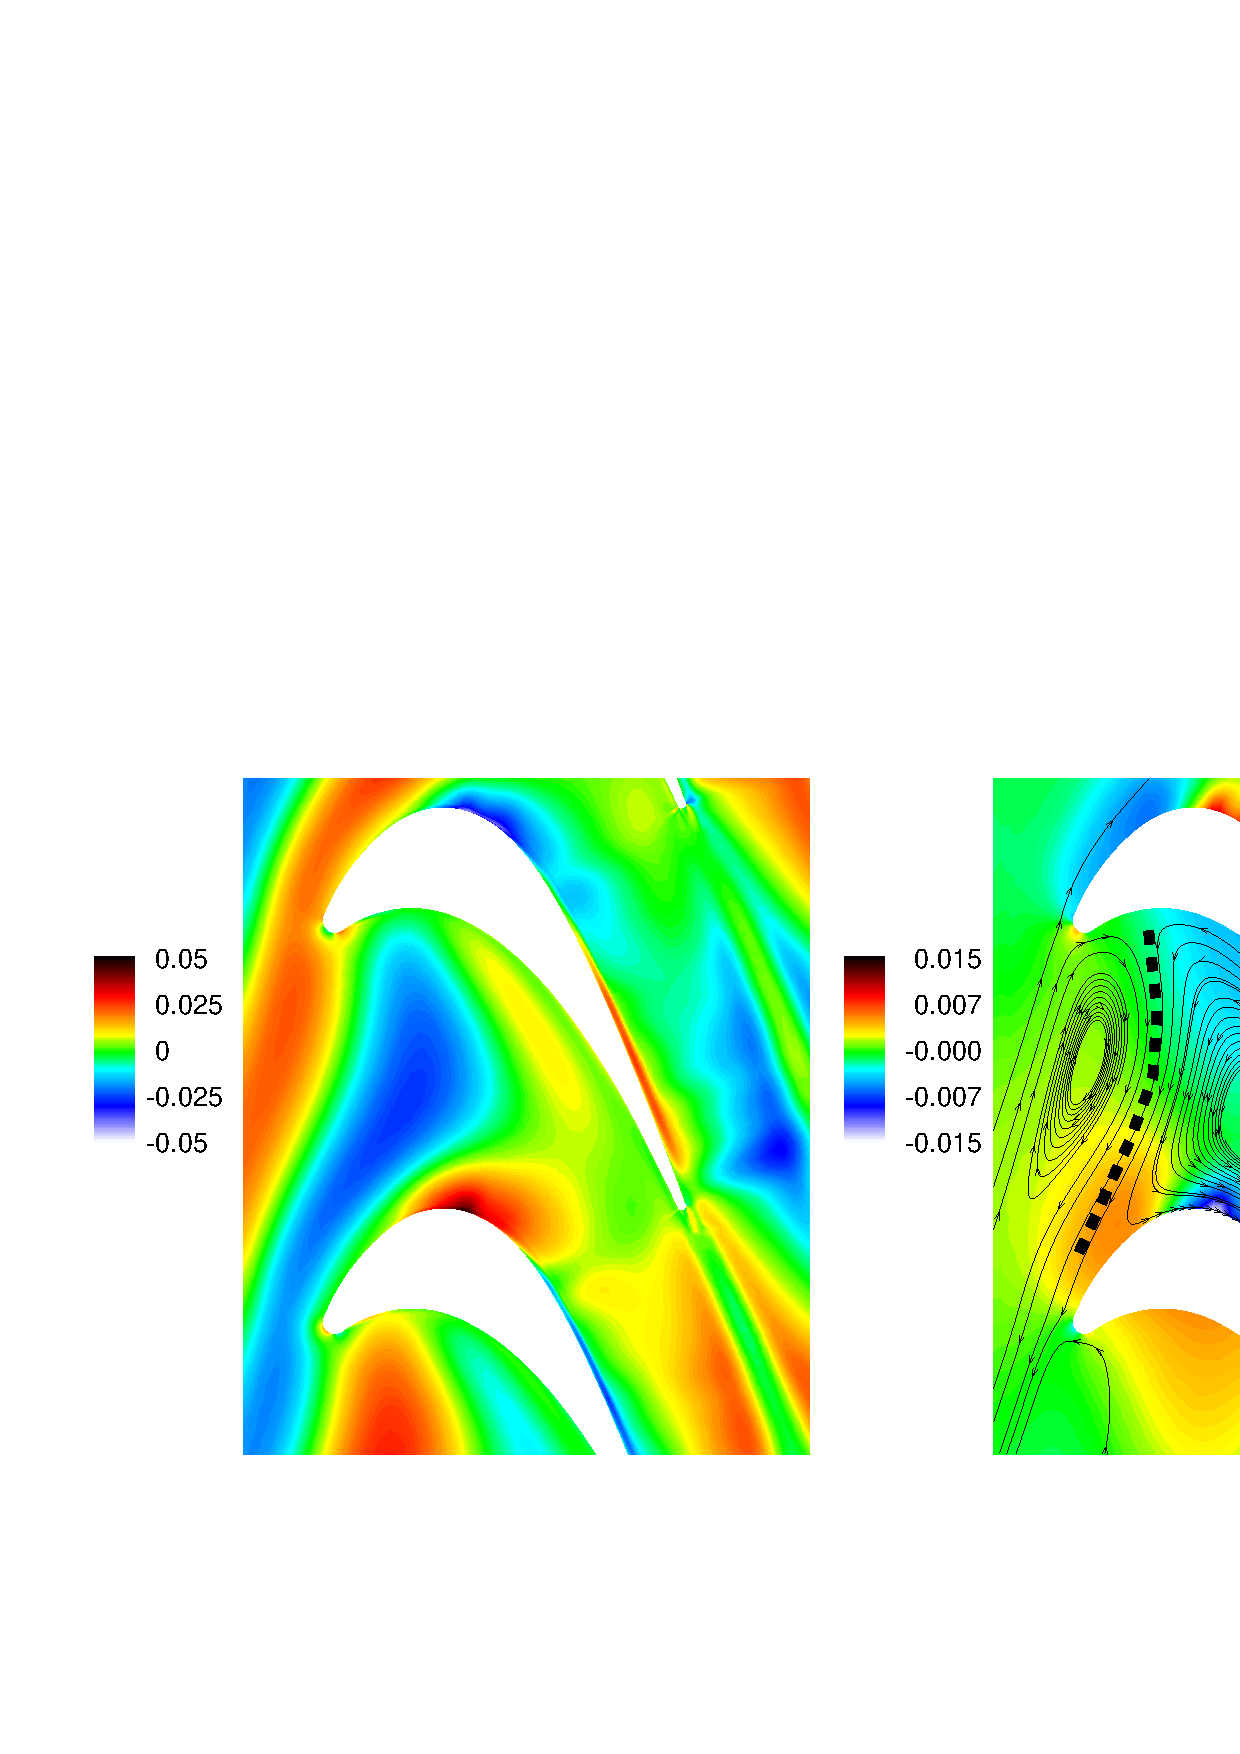
\includegraphics[width=130mm,clip=t]{CHAP_RT27/FIGURE/unsmidsec_4.pdf}}
       \\
     \subfigure[t = 1/6]
       {\hspace{-5mm}
        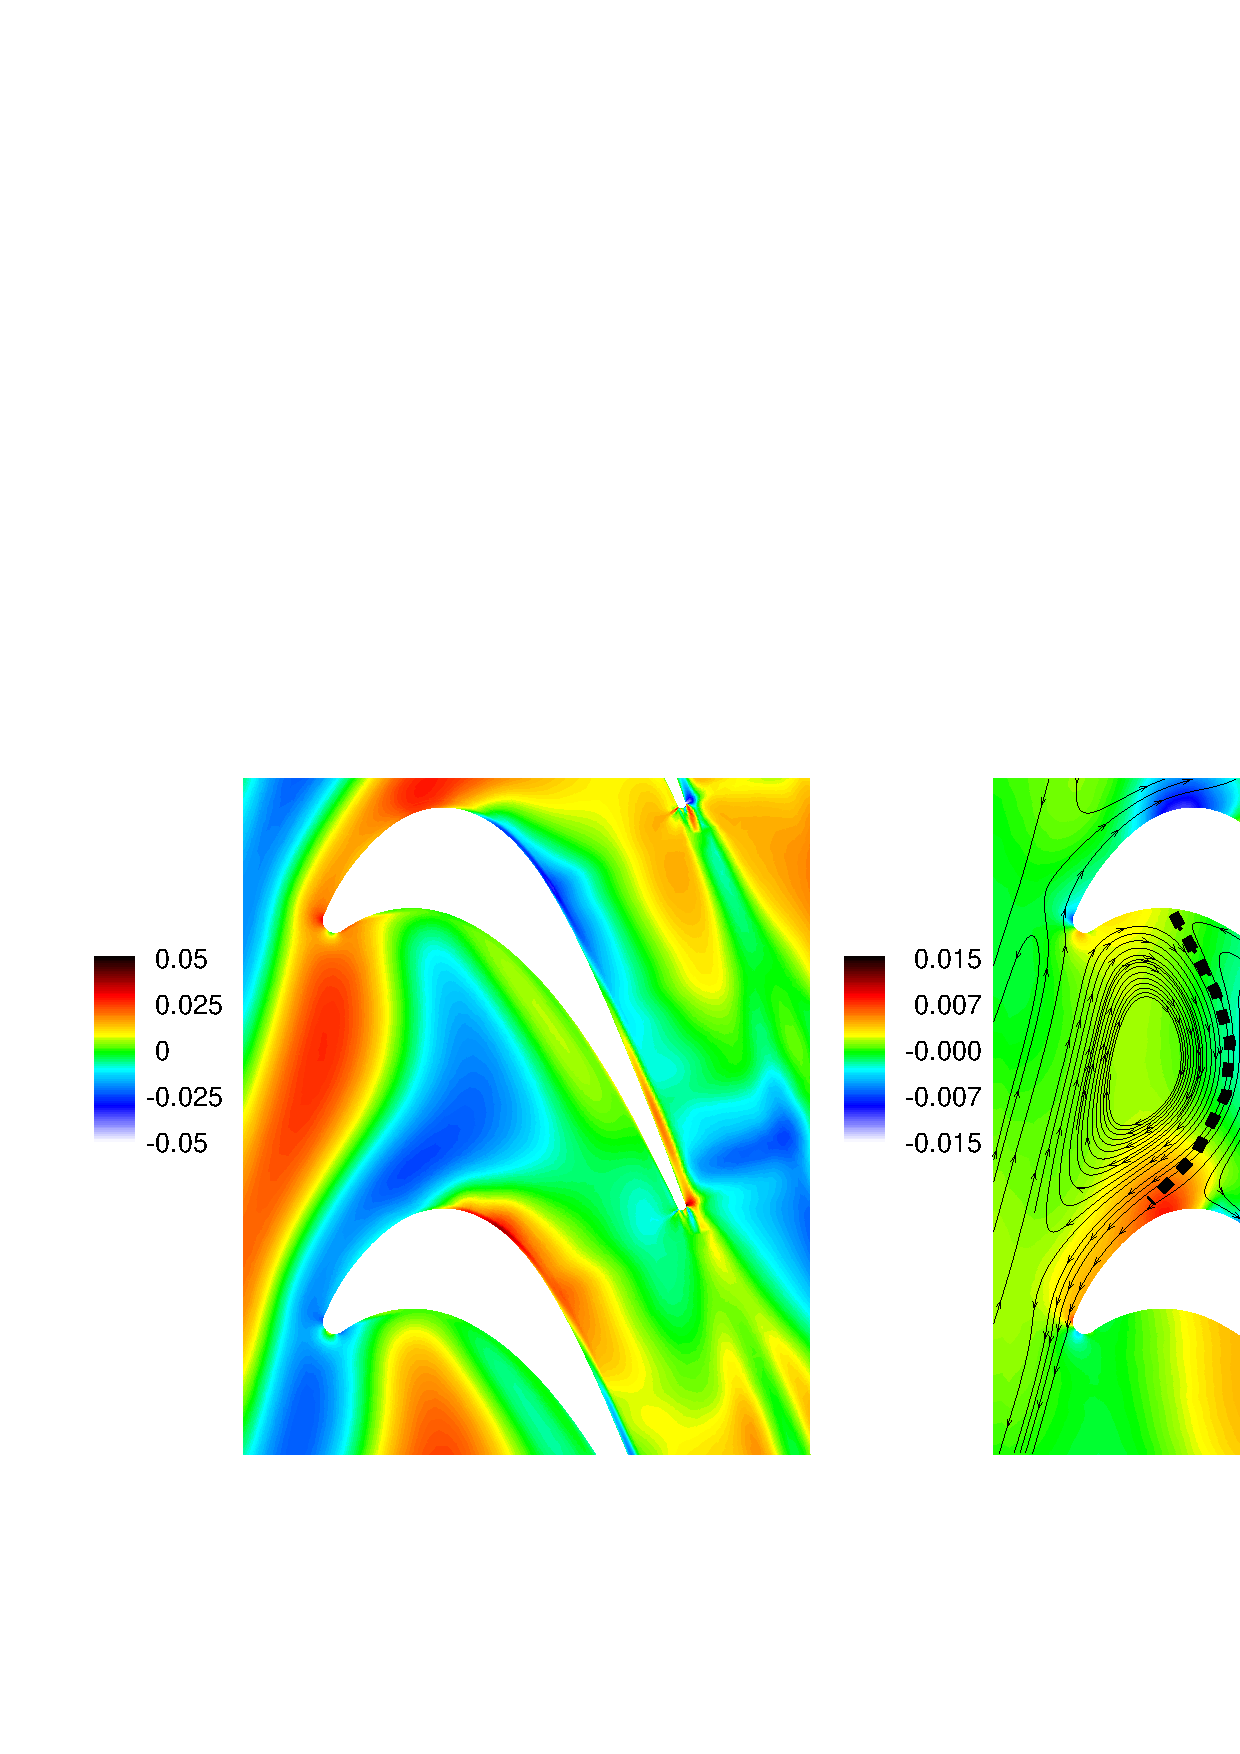
\includegraphics[width=130mm,clip=t]{CHAP_RT27/FIGURE/unsmidsec_5.pdf}}
       \\
     \subfigure[t = 2/6]
       {\hspace{-5mm}
        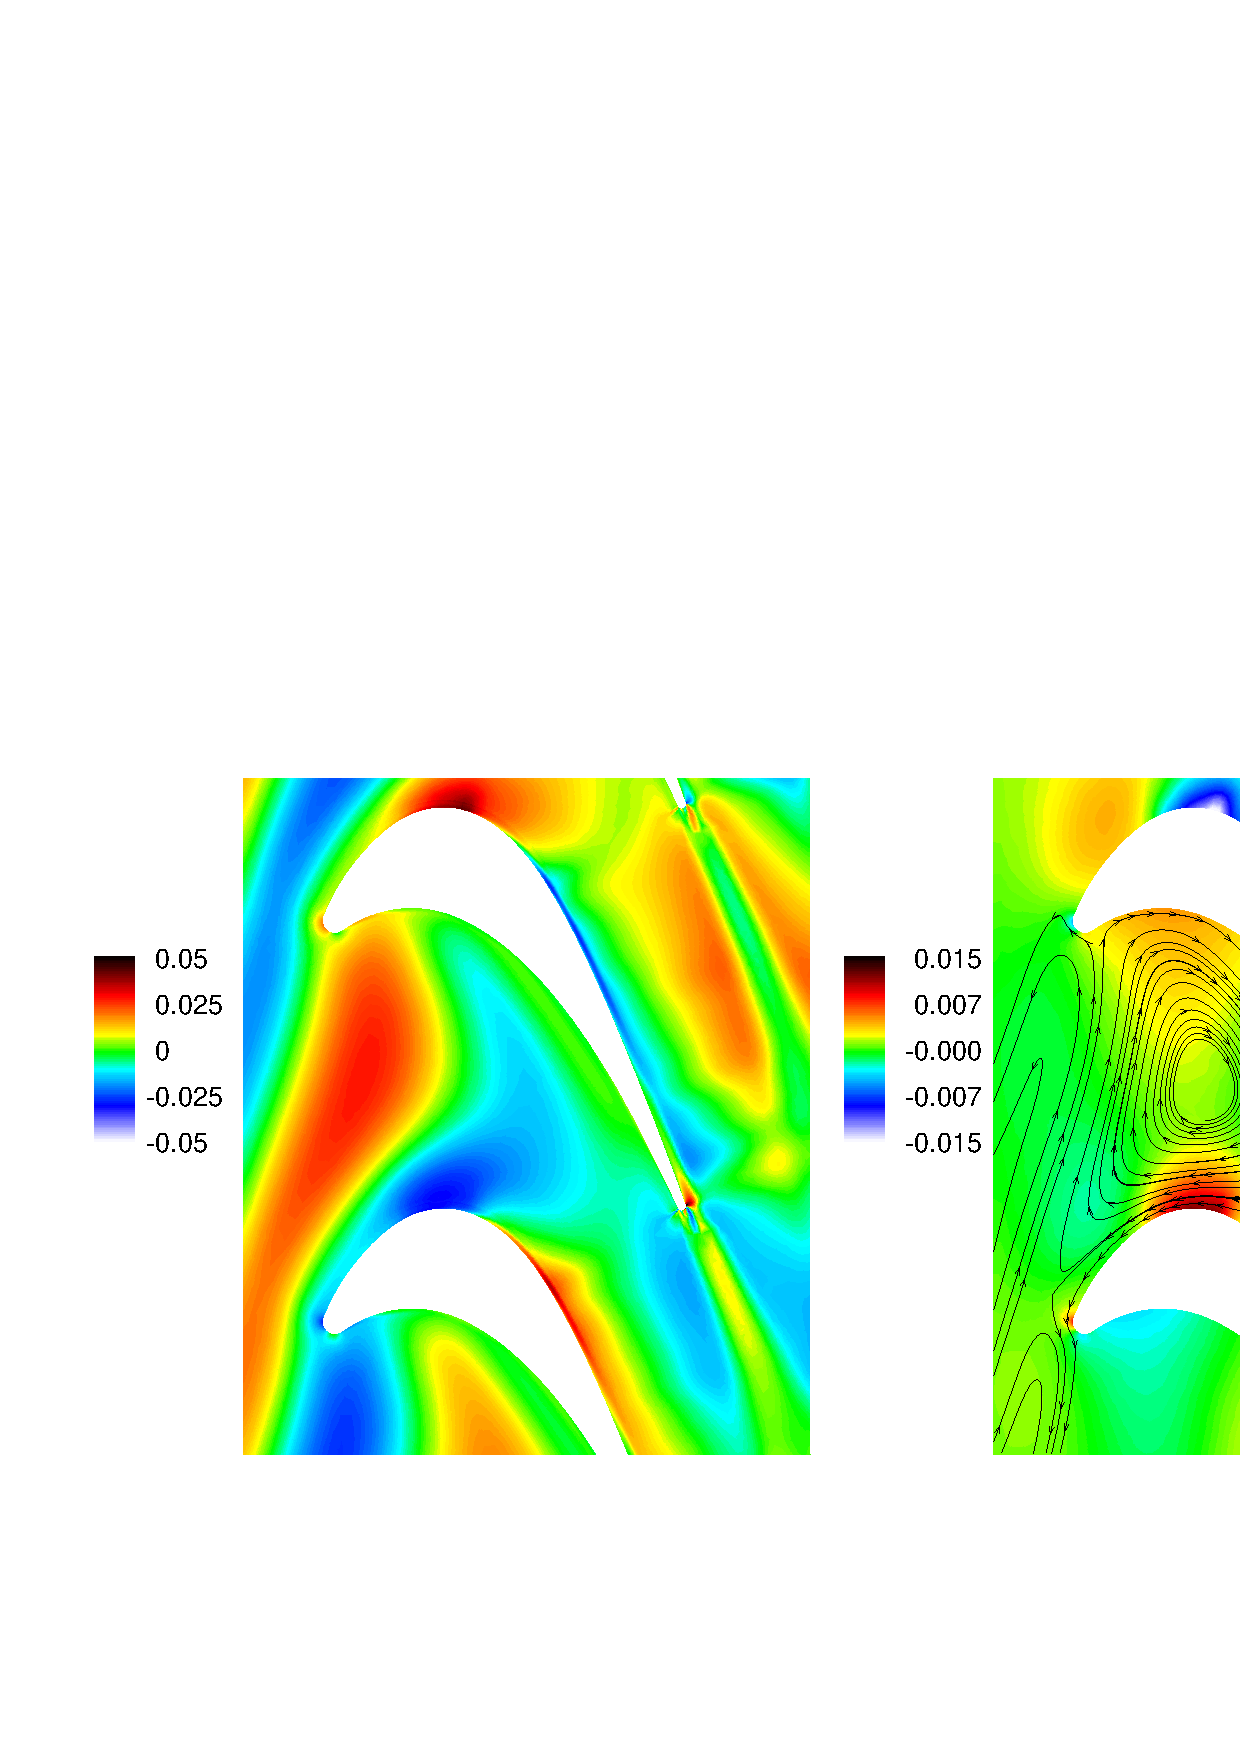
\includegraphics[width=130mm,clip=t]{CHAP_RT27/FIGURE/unsmidsec_6.pdf}}
   \end{tabular}
  \end{center}
  \vspace{-8mm}
  \caption{Vortical-flow interaction in the RT27a rotor passage at
           mid-height section (first Fourier component).
           Unsteady dimensionless absolute velocity fluctuations (left) and
           unsteady particle traces
           superimposed on dimensionless unsteady pressure fluctuations (right)}
  \label{rt27_vortical2d_1.fig}
\end{figure}
%
\begin{figure}
  \begin{center}
   \begin{tabular}{c}
     \subfigure[t = 3/6]
       {\hspace{-5mm}
        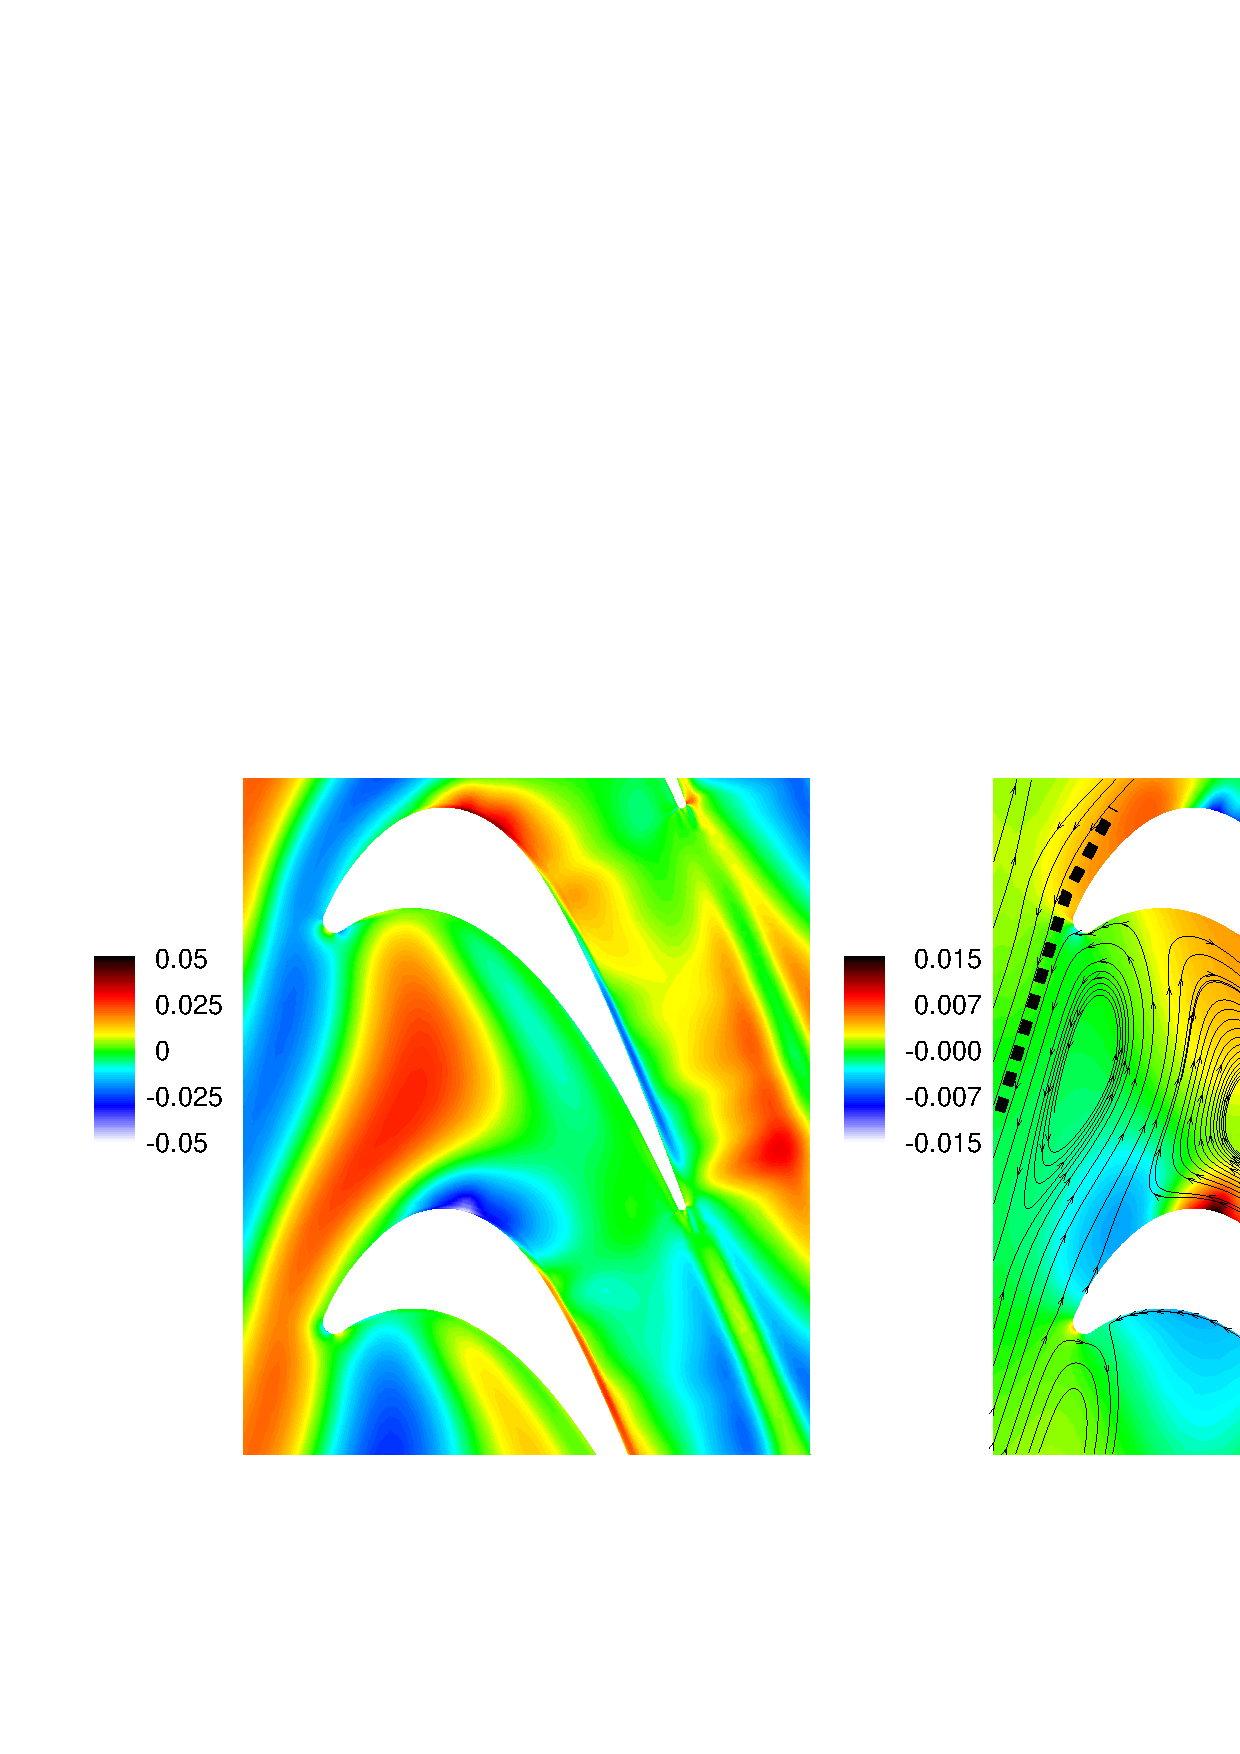
\includegraphics[width=130mm,clip=t]{CHAP_RT27/FIGURE/unsmidsec_1.pdf}}
       \\
     \subfigure[t = 4/6]
       {\hspace{-5mm}
        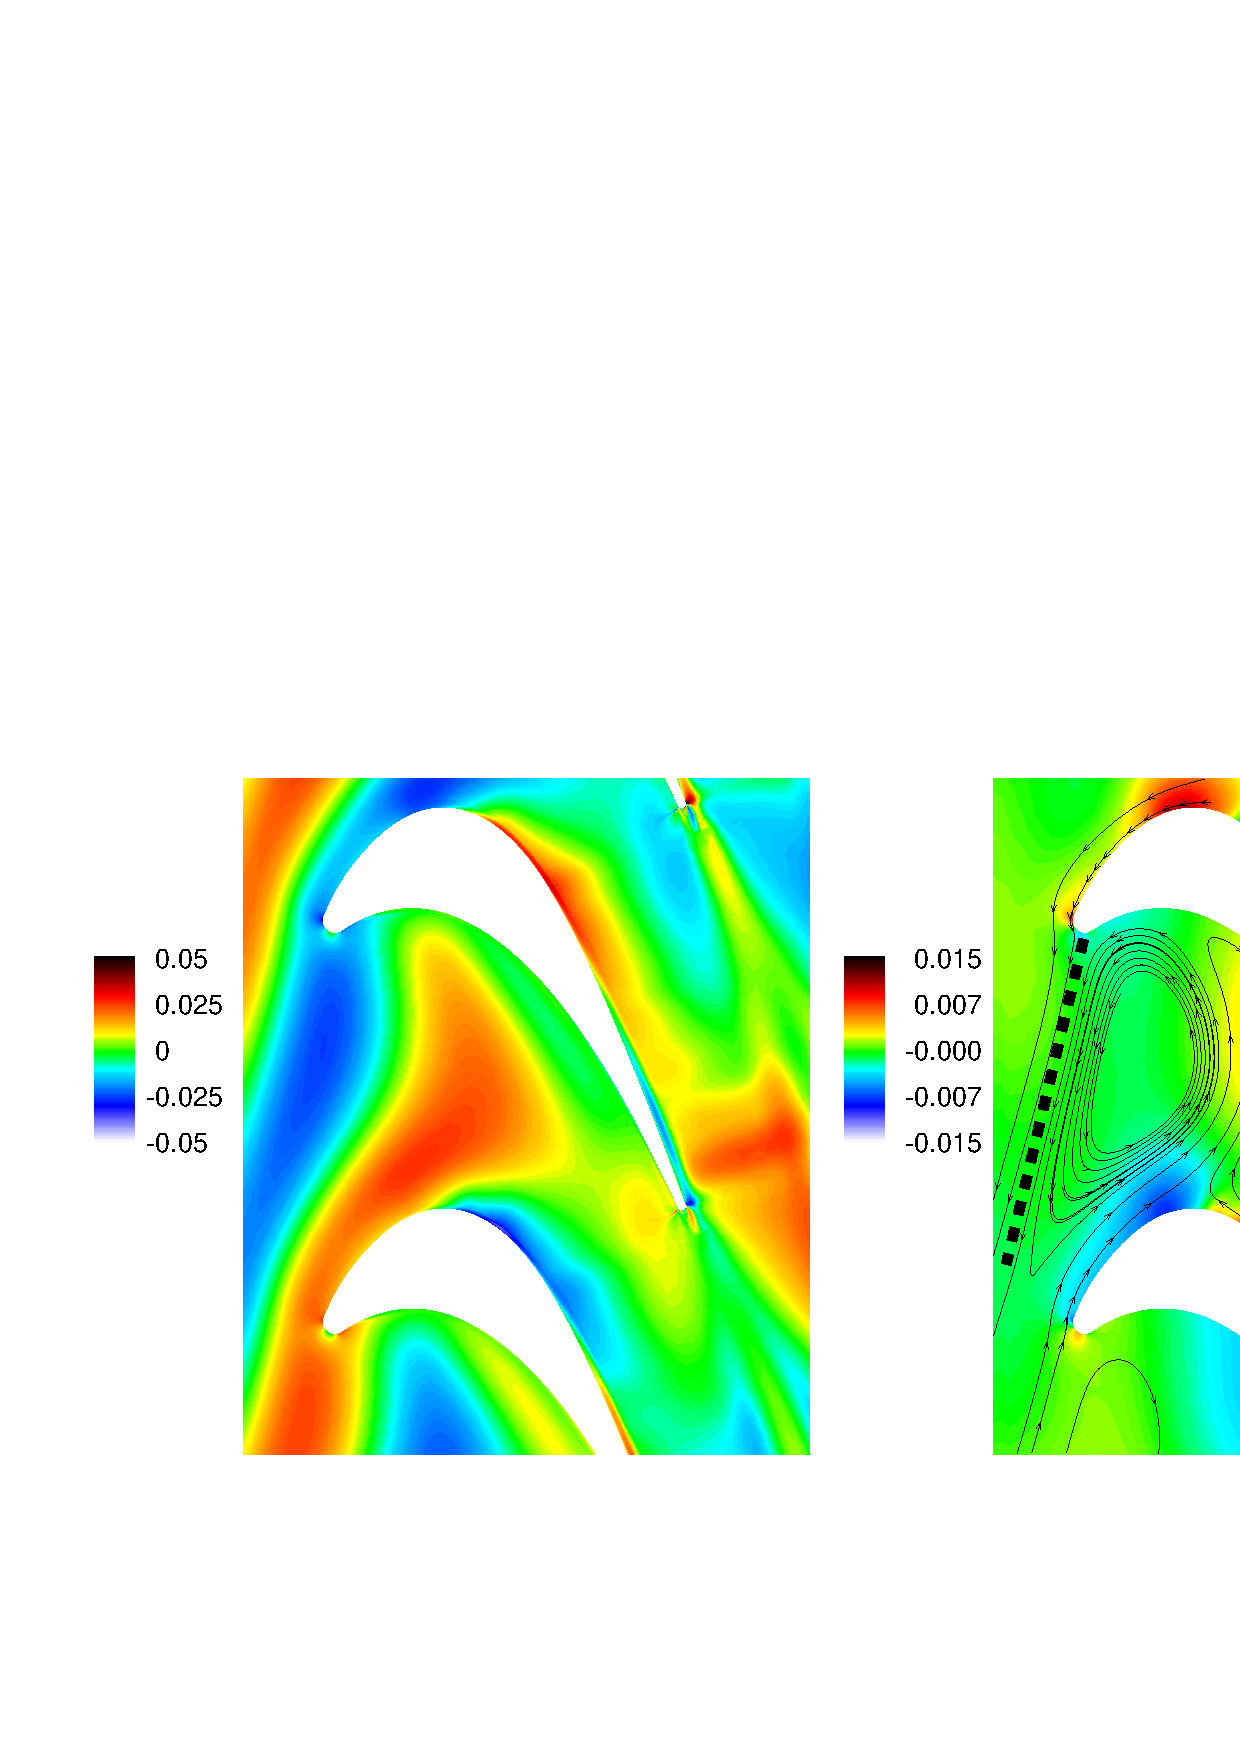
\includegraphics[width=130mm,clip=t]{CHAP_RT27/FIGURE/unsmidsec_2.pdf}}
       \\
     \subfigure[t = 5/6]
       {\hspace{-5mm}
        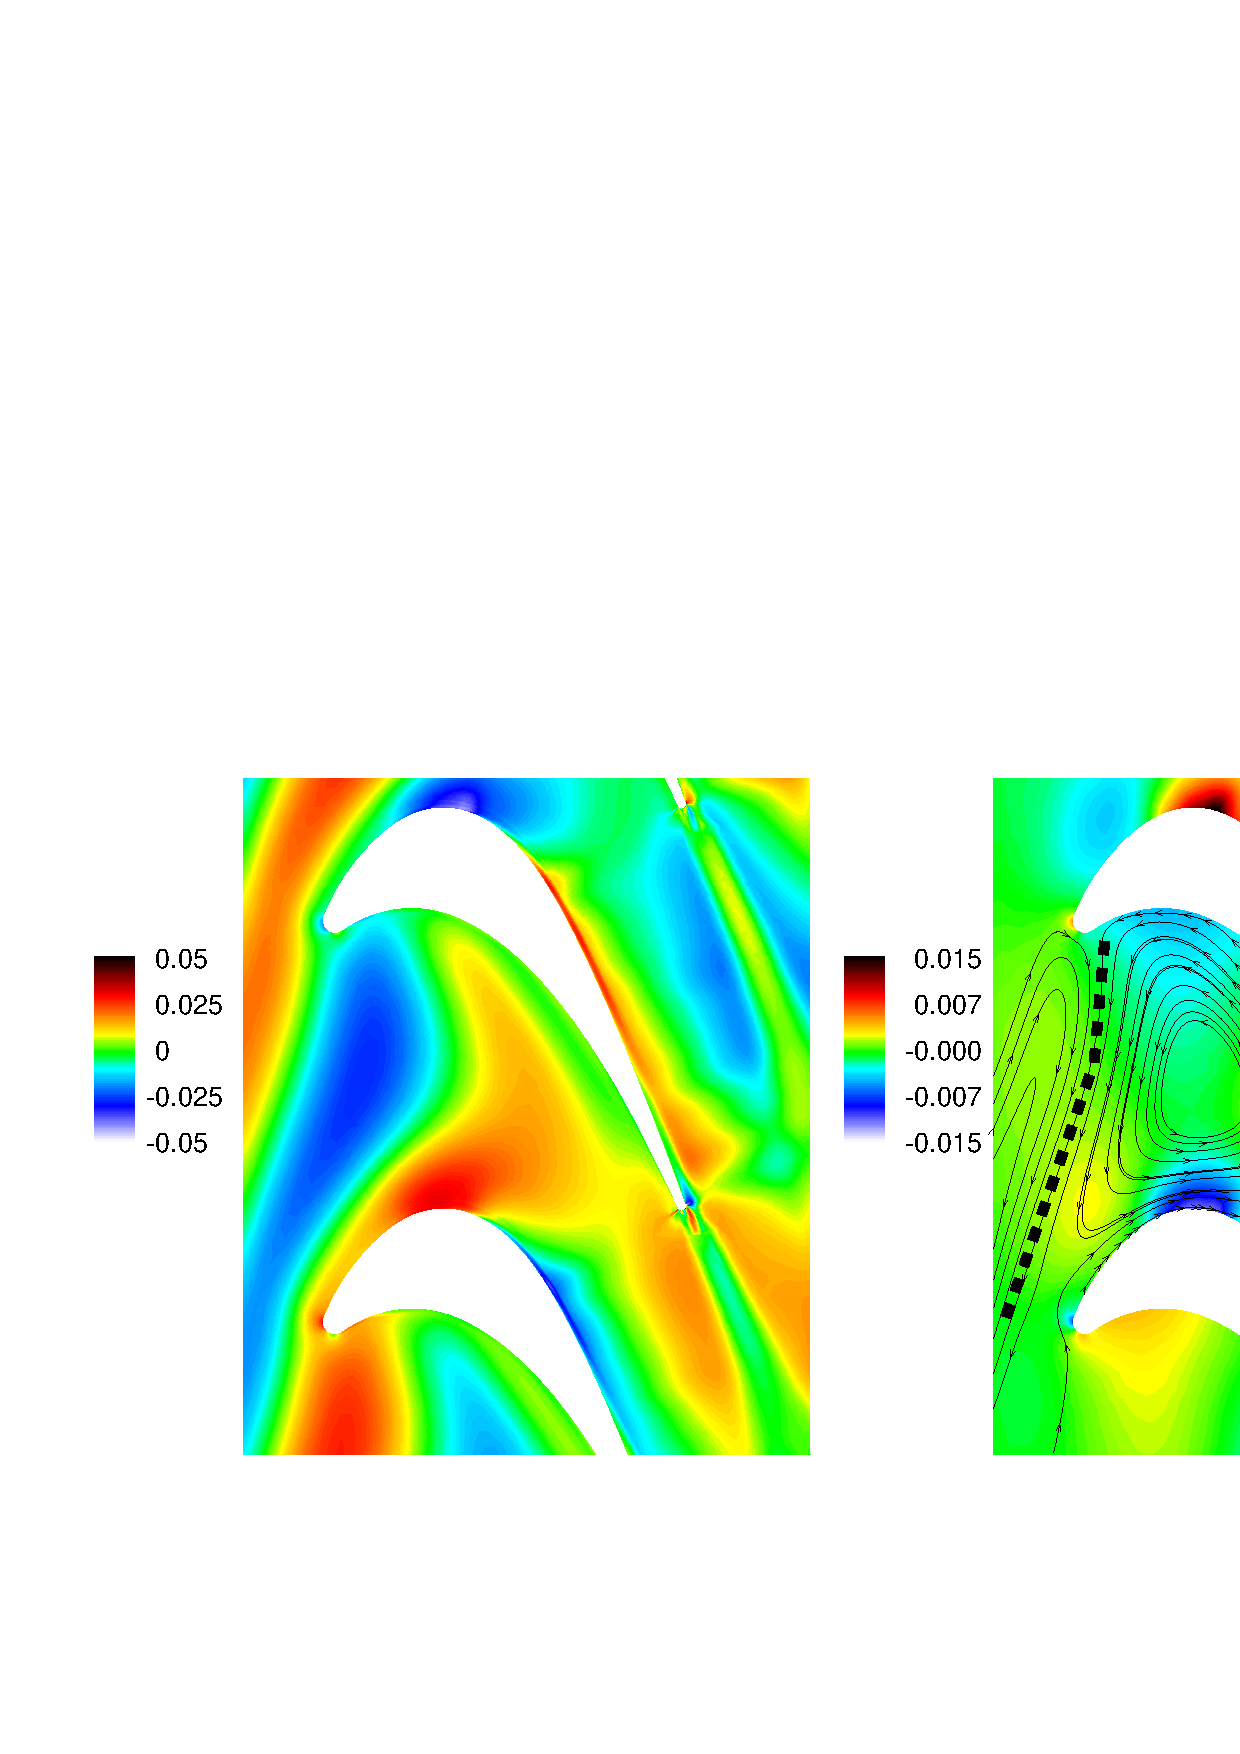
\includegraphics[width=130mm,clip=t]{CHAP_RT27/FIGURE/unsmidsec_3.pdf}}
   \end{tabular}
  \end{center}
  \vspace{-8mm}
  \caption{Vortical-flow interaction in the RT27a rotor passage at
           mid-height section (first Fourier component) continued.
           Unsteady dimensionless
           absolute velocity fluctuations (left) and unsteady particle traces
           superimposed on dimensionless unsteady pressure fluctuations (right)}
  \label{rt27_vortical2d_2.fig}
\end{figure}
%
 These recirculating flow patterns, generated as the wake is being cut, result
 in a counterclockwise rotating vortex downstream the wake centerline
 (indicated with a dotted line) and in a clockwise vortex upstream
 the centerline (Fig. \ref{rt27_vortical2d_1.fig}a).
 The upstream unsteady vortex is associated with a local increase of pressure
 while the downstream counterclockwise flow pattern causes a local decrease
 in pressure.
 After the wake is cut, a segment of wake is produced in the rotor passage and
 the two ends of the segment travel at local steady fluid speed. Since the flow
 is faster at the suction side, the wake centerline begins a counterclockwise
 rotation as it moves through the rotor passage.
 At the same time, the lower momentum fluid moves from the wake
 end near the pressure side to the wake end near the
 suction side, causing a thicker wake in the suction side and a thinner one in the
 pressure side (this is due to the direction of rotation of the two vortices).
 Broadly speaking, as the wake centerline moves downstream in the rotor passage,
 its influence in the unsteady pressure fluctuation tends to be
 more pronounced on the suction side of the blade. This is evident in
 the blade crown were the unsteady pressure amplitudes reach their maximum.
 As the recirculating flow patterns moves downstream, the wake is sheared,
 distorted and enlarged while the amplitude of the unsteady pressure
 is decreased and its region of influence increased.
 Near the trailing-edge of the blade, there is an expansion region
 on the suction side which causes a local increase in pressure amplitude
 across the the line of the trailing-edges. This is also evident from
 Fig. \ref{rt27_unsteady3d_1.fig}b in the region $0.5<x/c\sm{x}<0.75$.

~\newline
 Fig. \ref{rt27_vortical1_3d.fig}a shows the unsteady pressure
 amplitude computed by using the first Fourier harmonic of
 vortical flow component at the NGV outlet.
 The pressure surface exhibits more 3D features
 than the suction surface.
 The amplitude of disturbances on the pressure surface is higher
 towards the forward part of the root section. This because of
 the stronger vortical field indicated in
 Fig. \ref{ngv_outlet_decomposed1.fig}a. On the other hand the
 resistance of the wake effect is reduced if compared with mid-height
 and tip sections (blue region at the root trailing-edge
 in Fig. \ref{rt27_vortical1_3d.fig}a). The reason for this reduced resistance
 can be tracked to the lower wake exit angle at root section.
 Infact Korakianitis \citeyear{Kora:3} showed that the wakes
 from lower stator exit angles act for a shorter part of the blade passing cycle.
%
%
\begin{figure}
  \begin{center}
   \begin{tabular}{cc}
     \subfigure[Pressure surface]
       {\hspace{-5mm}
        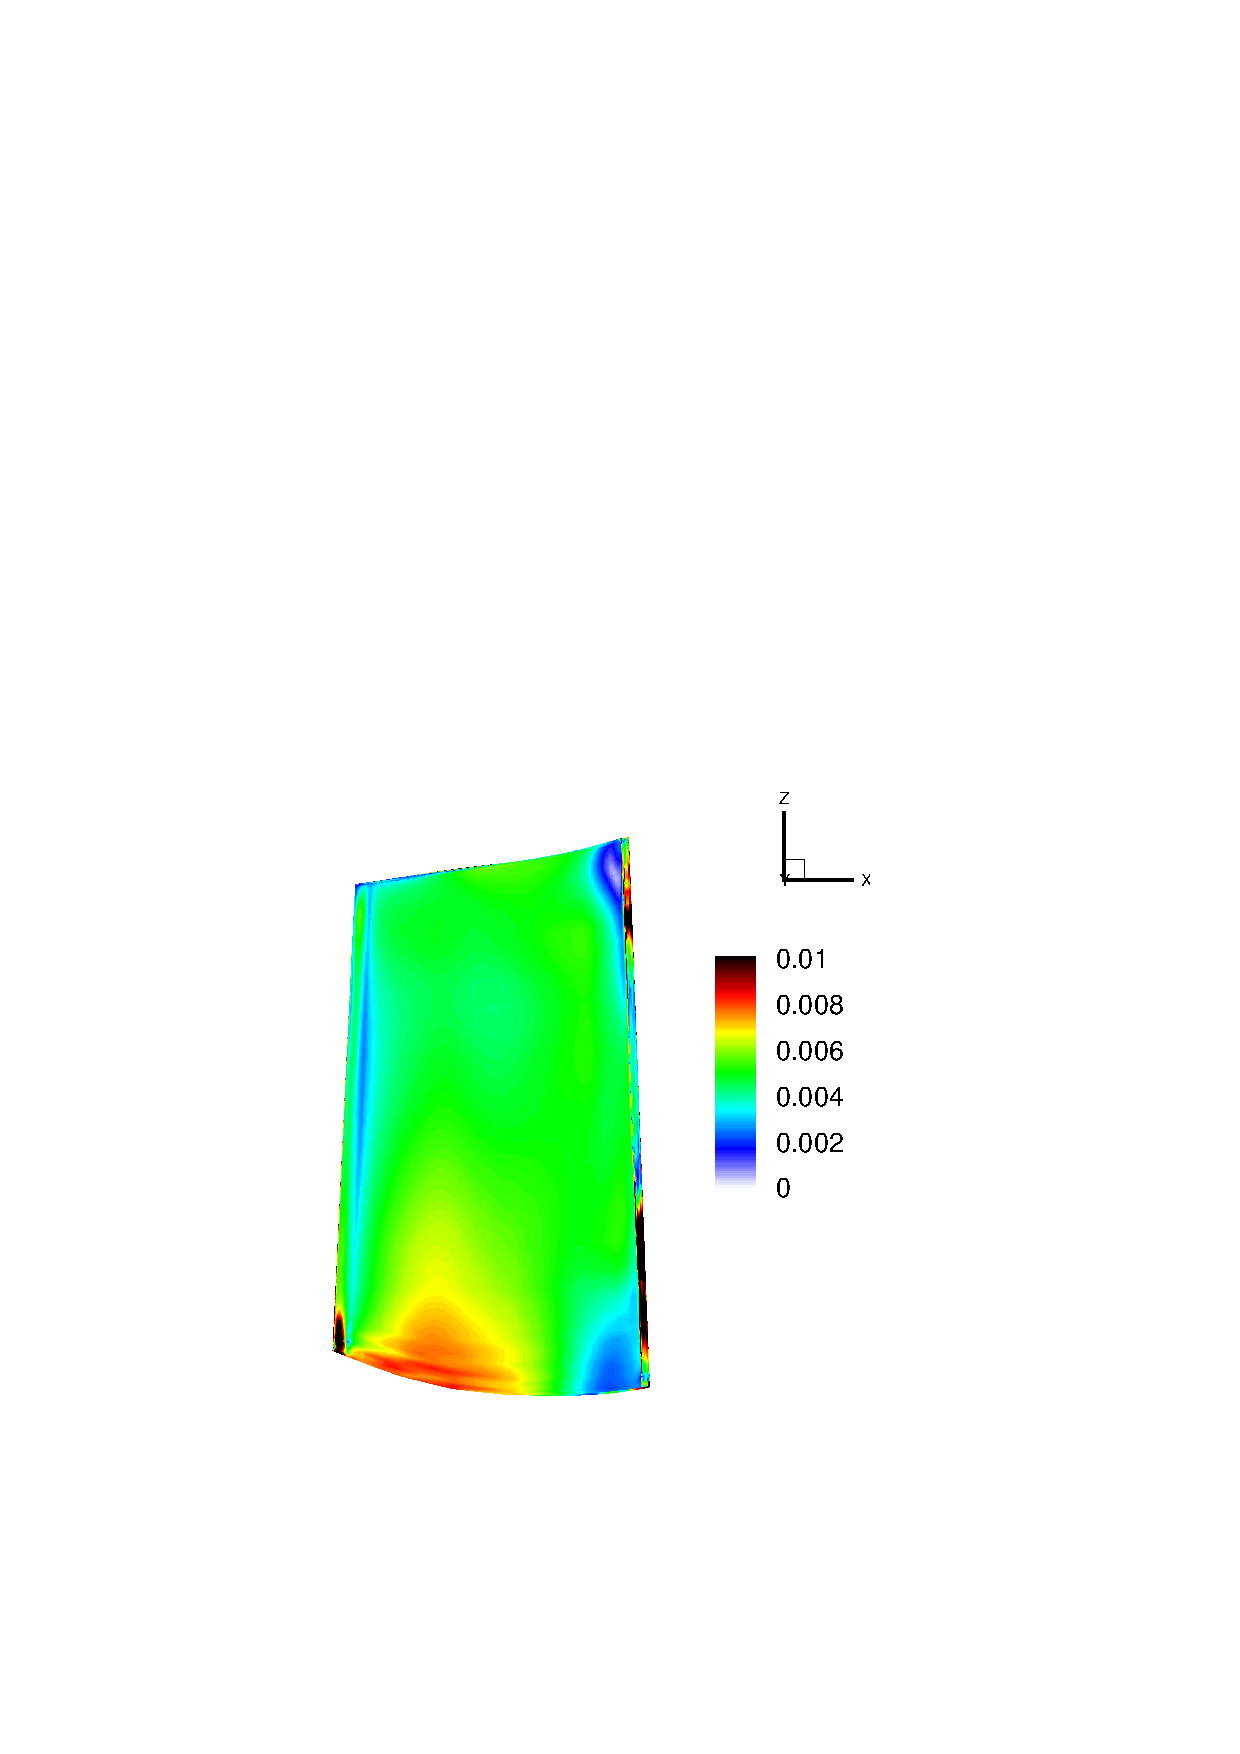
\includegraphics[width=70mm,clip=t]{CHAP_RT27/FIGURE/presvor1.pdf}}
       &
     \subfigure[Suction surface]
       {\hspace{-5mm}
        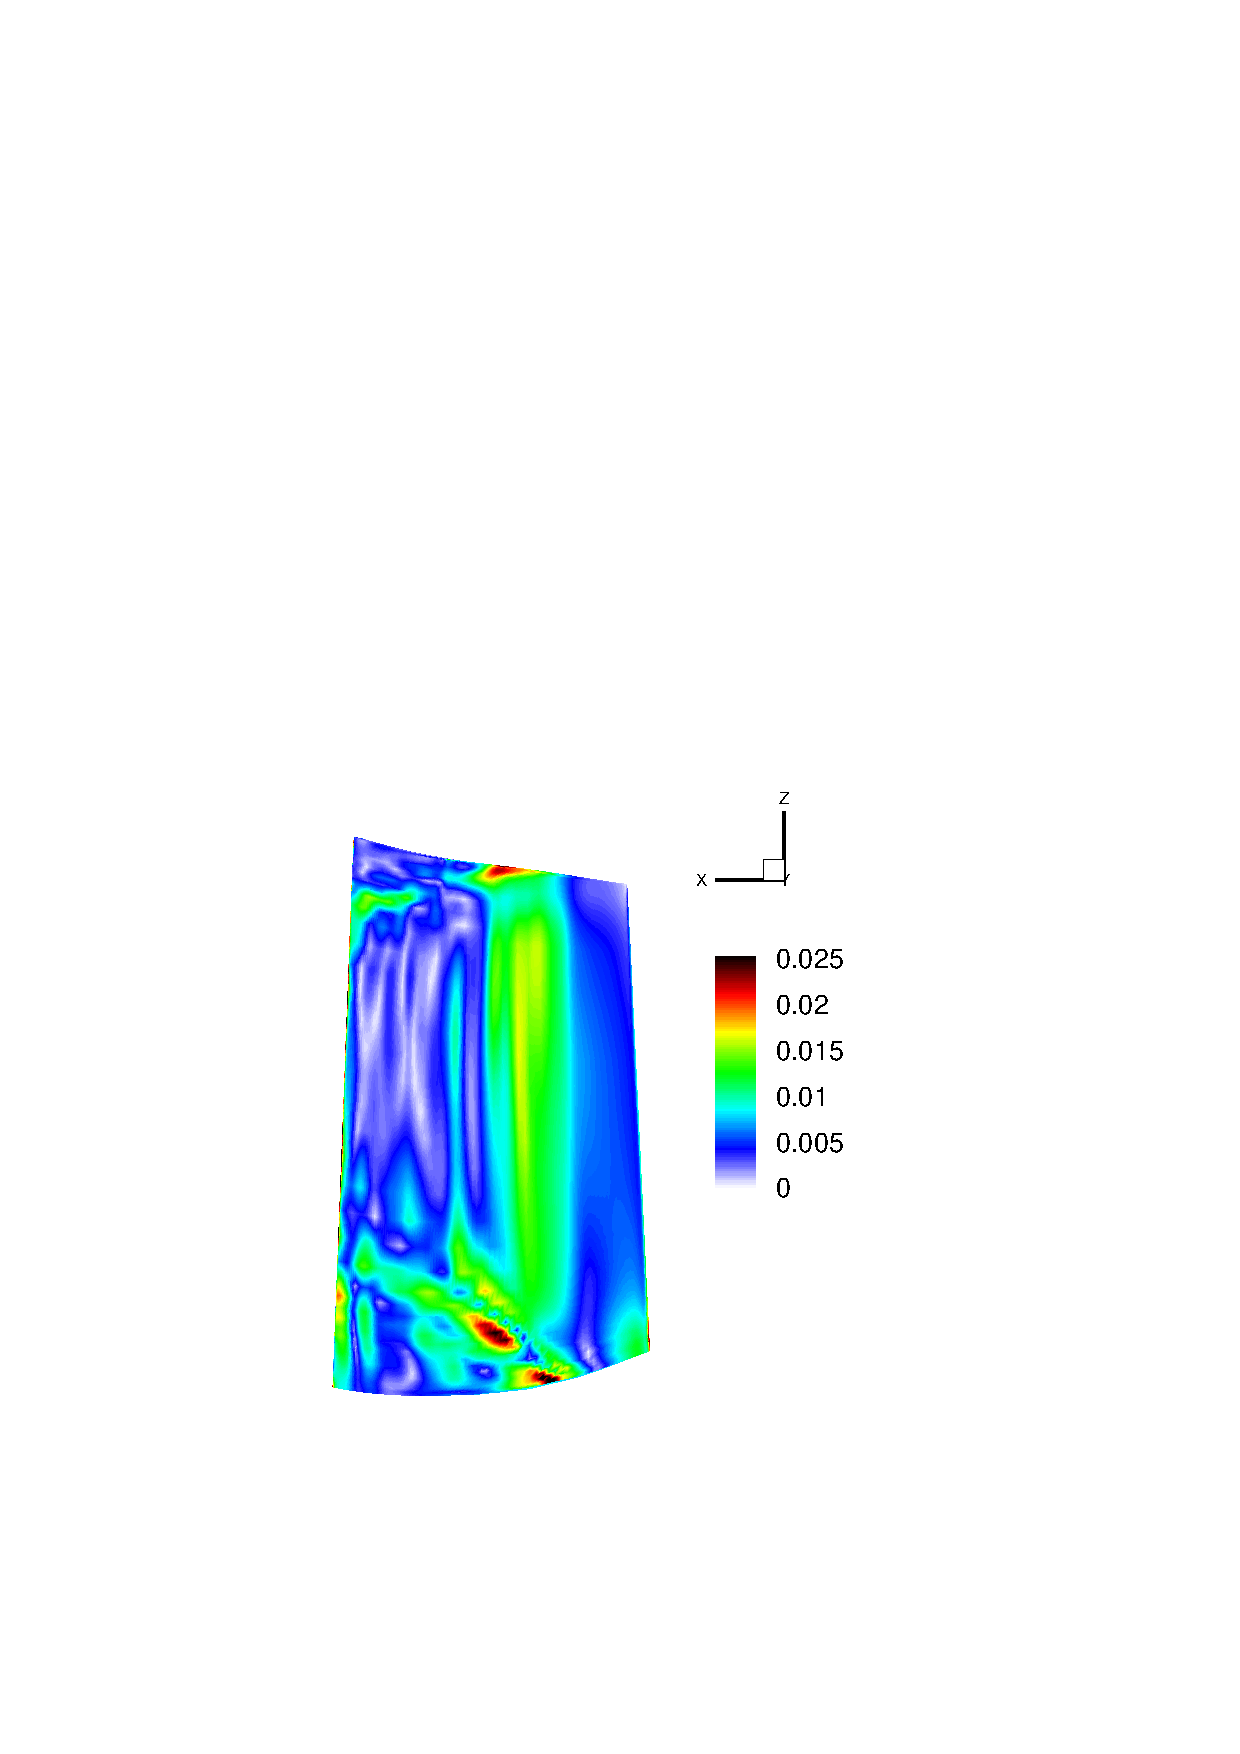
\includegraphics[width=70mm,clip=t]{CHAP_RT27/FIGURE/suctvor1.pdf}}
   \end{tabular}
  \end{center}
  \vspace{-8mm}
  \caption{Unsteady pressure on RT27a rotor blade due to
           Wake-rotor interaction (first Fourier component)}
  \label{rt27_vortical1_3d.fig}
\end{figure}
%
 On the suction surface, the perturbations reach their peak on the crown
 of the blade as shown in Fig. \ref{rt27_vortical1_3d.fig}b. In addition,
 a region of high pressure amplitude is noticeable in the region were
 the suction side separation line of the horseshoe vortex is located
 (see Fig. \ref{rotor_blade_traces.fig}b).
 The propagative aspect of the vortical flow interaction can be easily seen from
 an ispection of the unsteady pressure animation.
 The perturbation starts at the leading-edge and then propagates
 towards the rotor outlet with the steady-state local fluid velocity.
%
%
\begin{figure}
  \begin{center}
   \begin{tabular}{cc}
     \subfigure[Pressure surface]
       {\hspace{-5mm}
        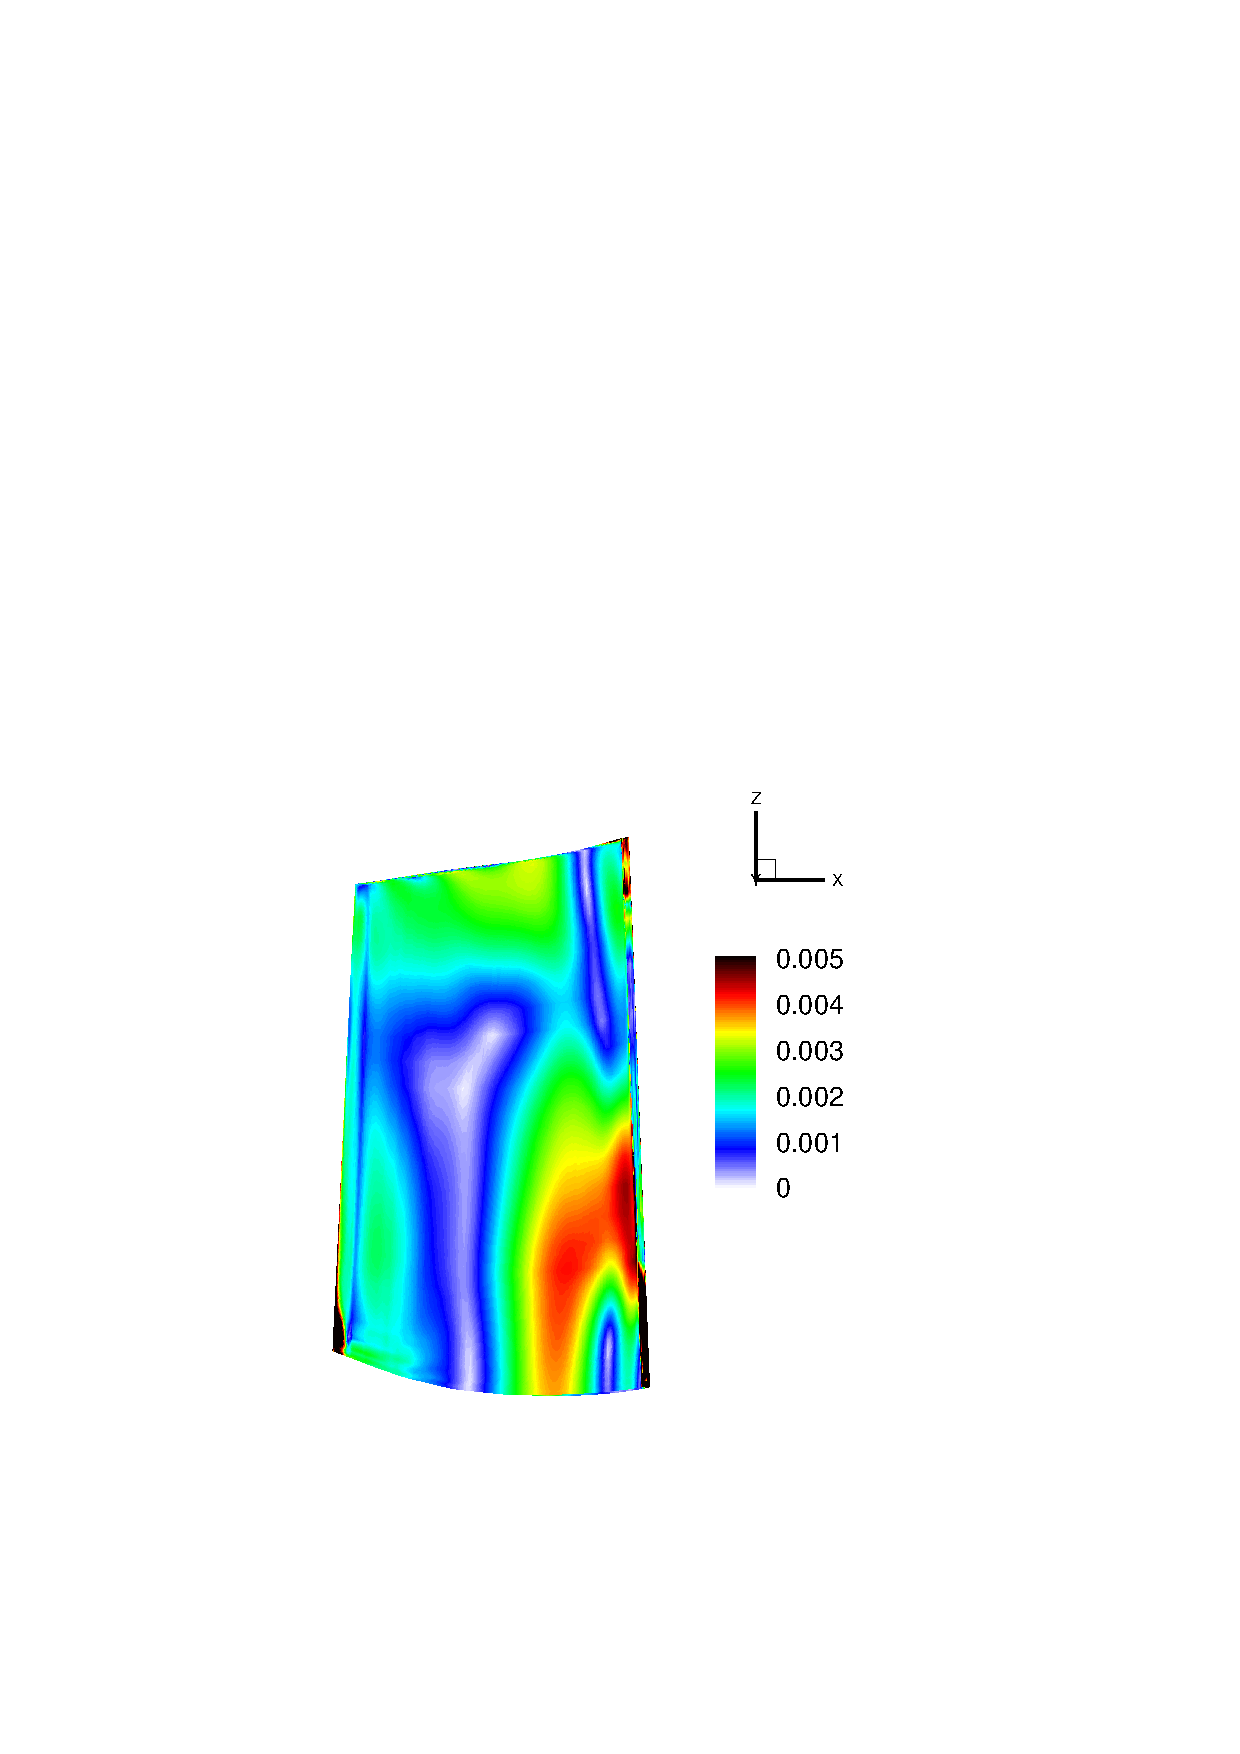
\includegraphics[width=70mm,clip=t]{CHAP_RT27/FIGURE/presvor2.pdf}}
       &
     \subfigure[Suction surface]
       {\hspace{-5mm}
        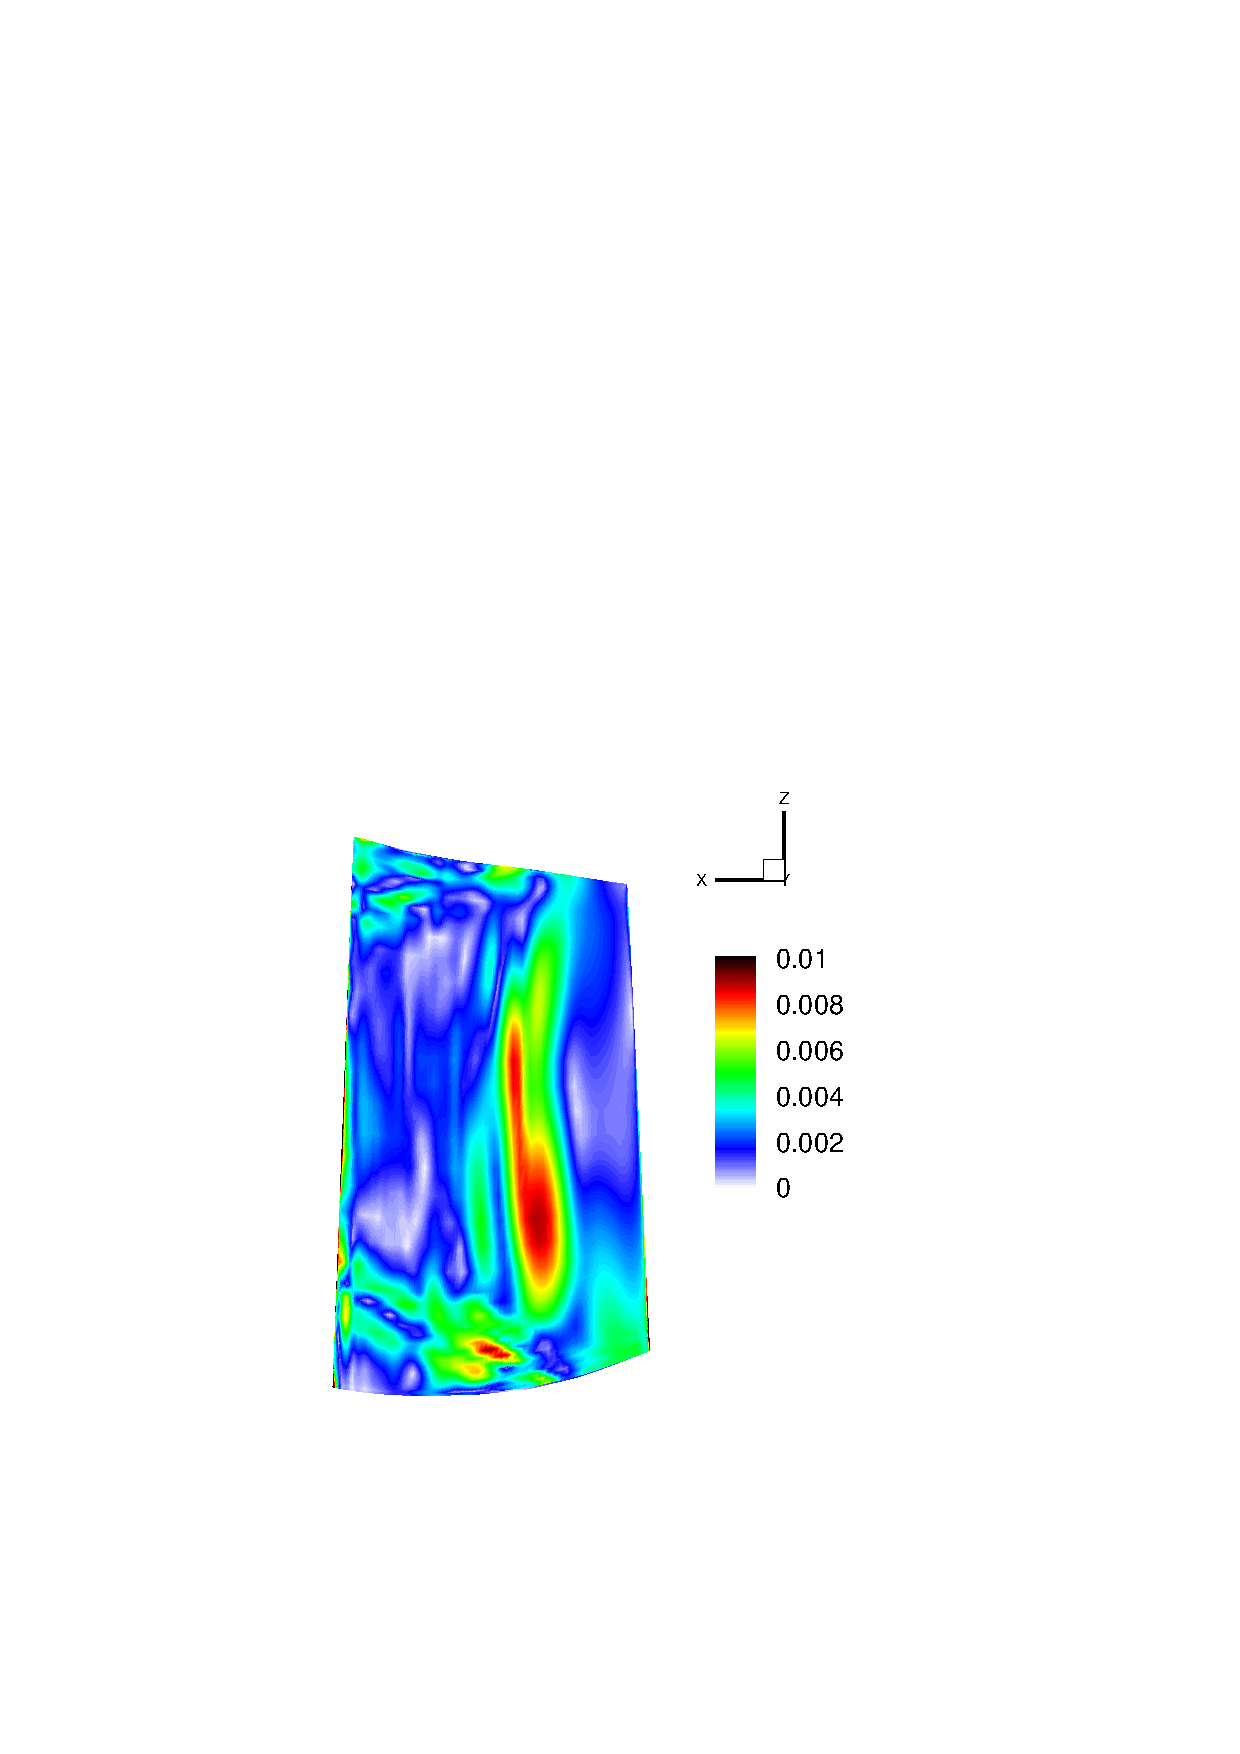
\includegraphics[width=70mm,clip=t]{CHAP_RT27/FIGURE/suctvor2.pdf}}
   \end{tabular}
  \end{center}
  \vspace{-8mm}
  \caption{Unsteady pressure on RT27a rotor blade due to
           Wake-rotor interaction (second Fourier component)}
  \label{rt27_vortical2_3d.fig}
\end{figure}

~\newline
 The unsteady pressure amplitude caused by the second Fourier
 component of the NGV-outlet vortical flow non-uniformities of
 Fig. \ref{ngv_outlet_decomposed1.fig}b is shown in
 Fig. \ref{rt27_vortical2_3d.fig}.
 The 3D effects are much stronger than those due to
 the the first Fourier harmonic,
 especially in the pressure surface where the
 pressure amplitude distribution differs significantly from
 Fig. \ref{rt27_vortical1_3d.fig}a. In contrast, the suction
 surface disturbances have a qualitatively similar behaviour to
 Fig. \ref{rt27_vortical1_3d.fig}b.
%
%
%
%
%
\subsection{Potential-flow interaction effects}
\label{rt27_potential.subsec}
%
 An analysis of the temporal variation of
 the potential-flow interaction is given in this section.
 The potential flow at the NGV outlet is shown in
 Fig. \ref{ngv_outlet_decomposed1.fig}b for the first two harmonics.
 Such a potential flow does not show particoular 3D
 features although its amplitude is higher
 towards the root section.
%
\begin{figure}
  \begin{center}
   \begin{tabular}{cc}
     \subfigure[Pressure surface]
       {\hspace{-5mm}
        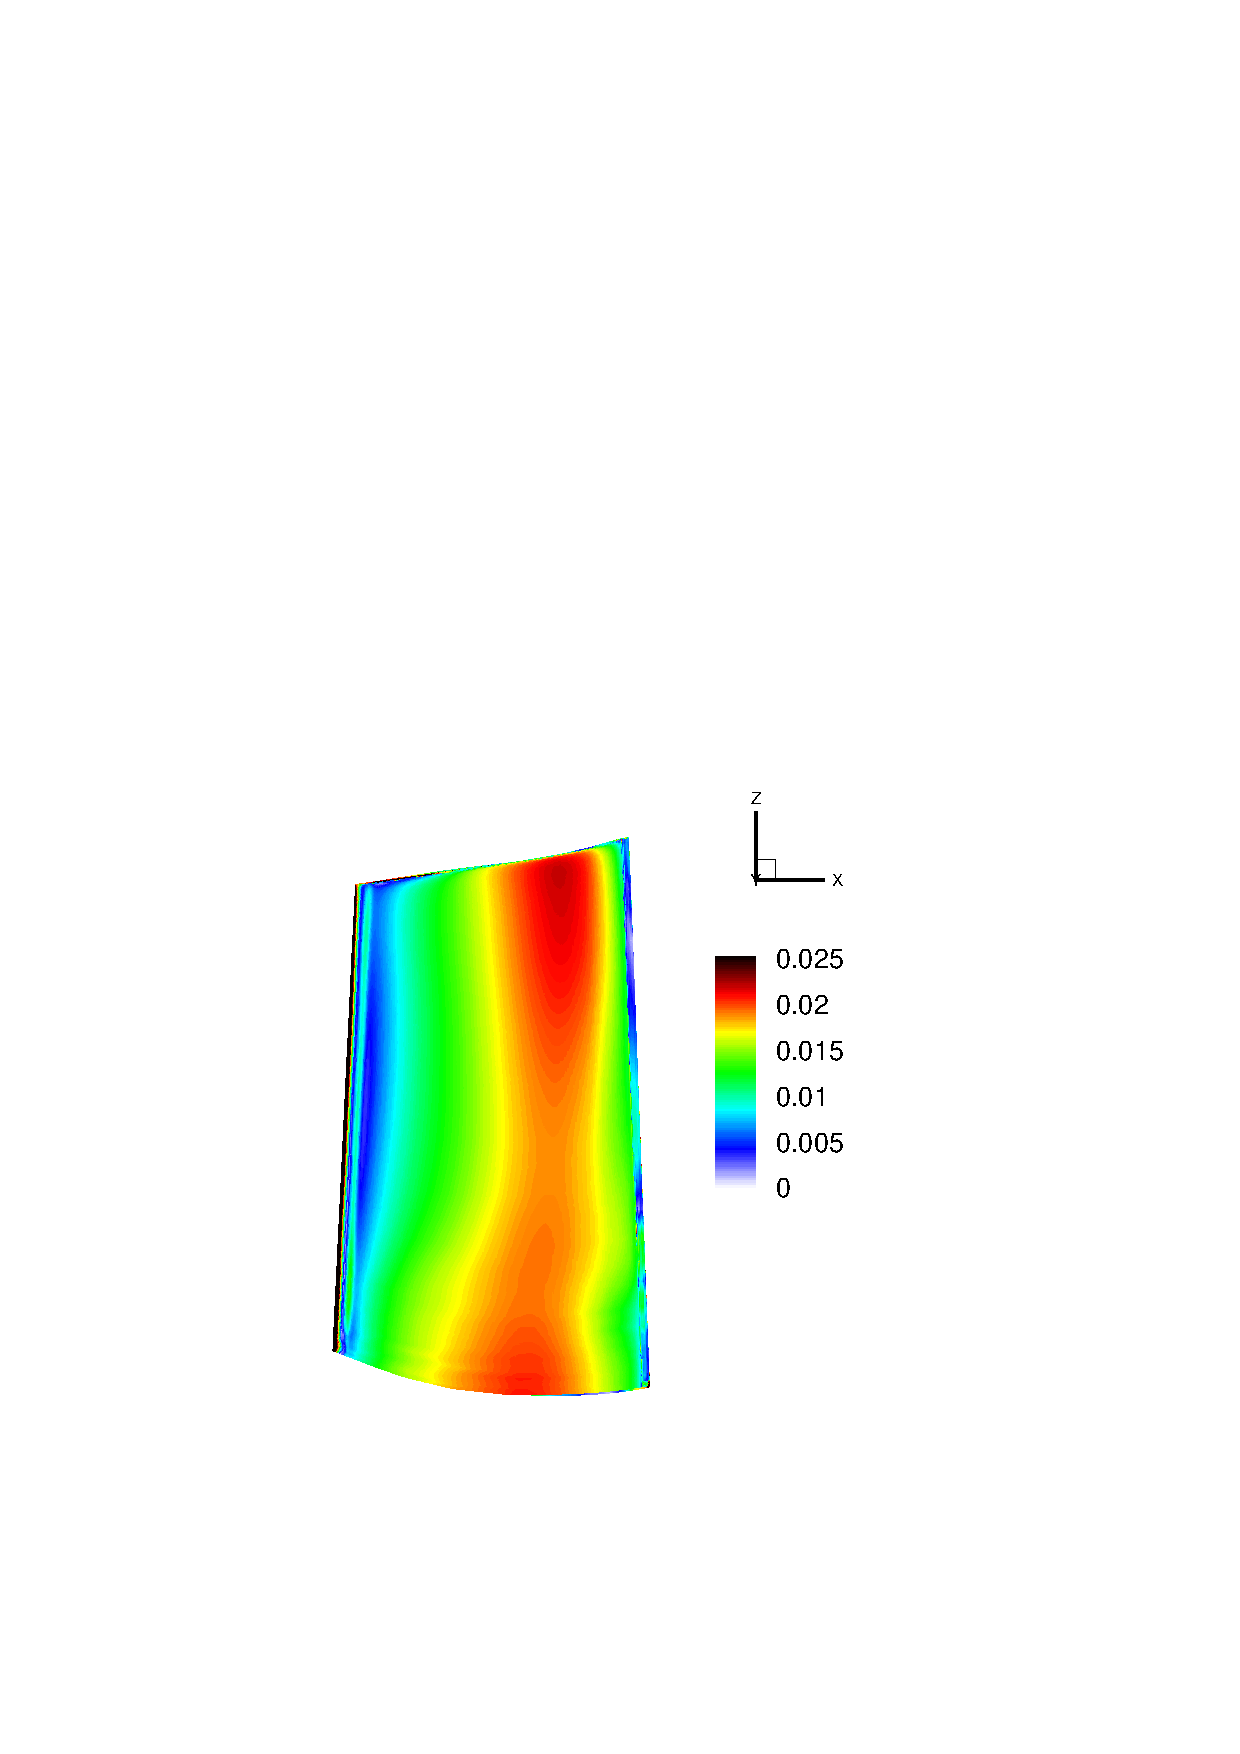
\includegraphics[width=70mm,clip=t]{CHAP_RT27/FIGURE/prespot1.pdf}}
       &
     \subfigure[Suction surface]
       {\hspace{-5mm}
        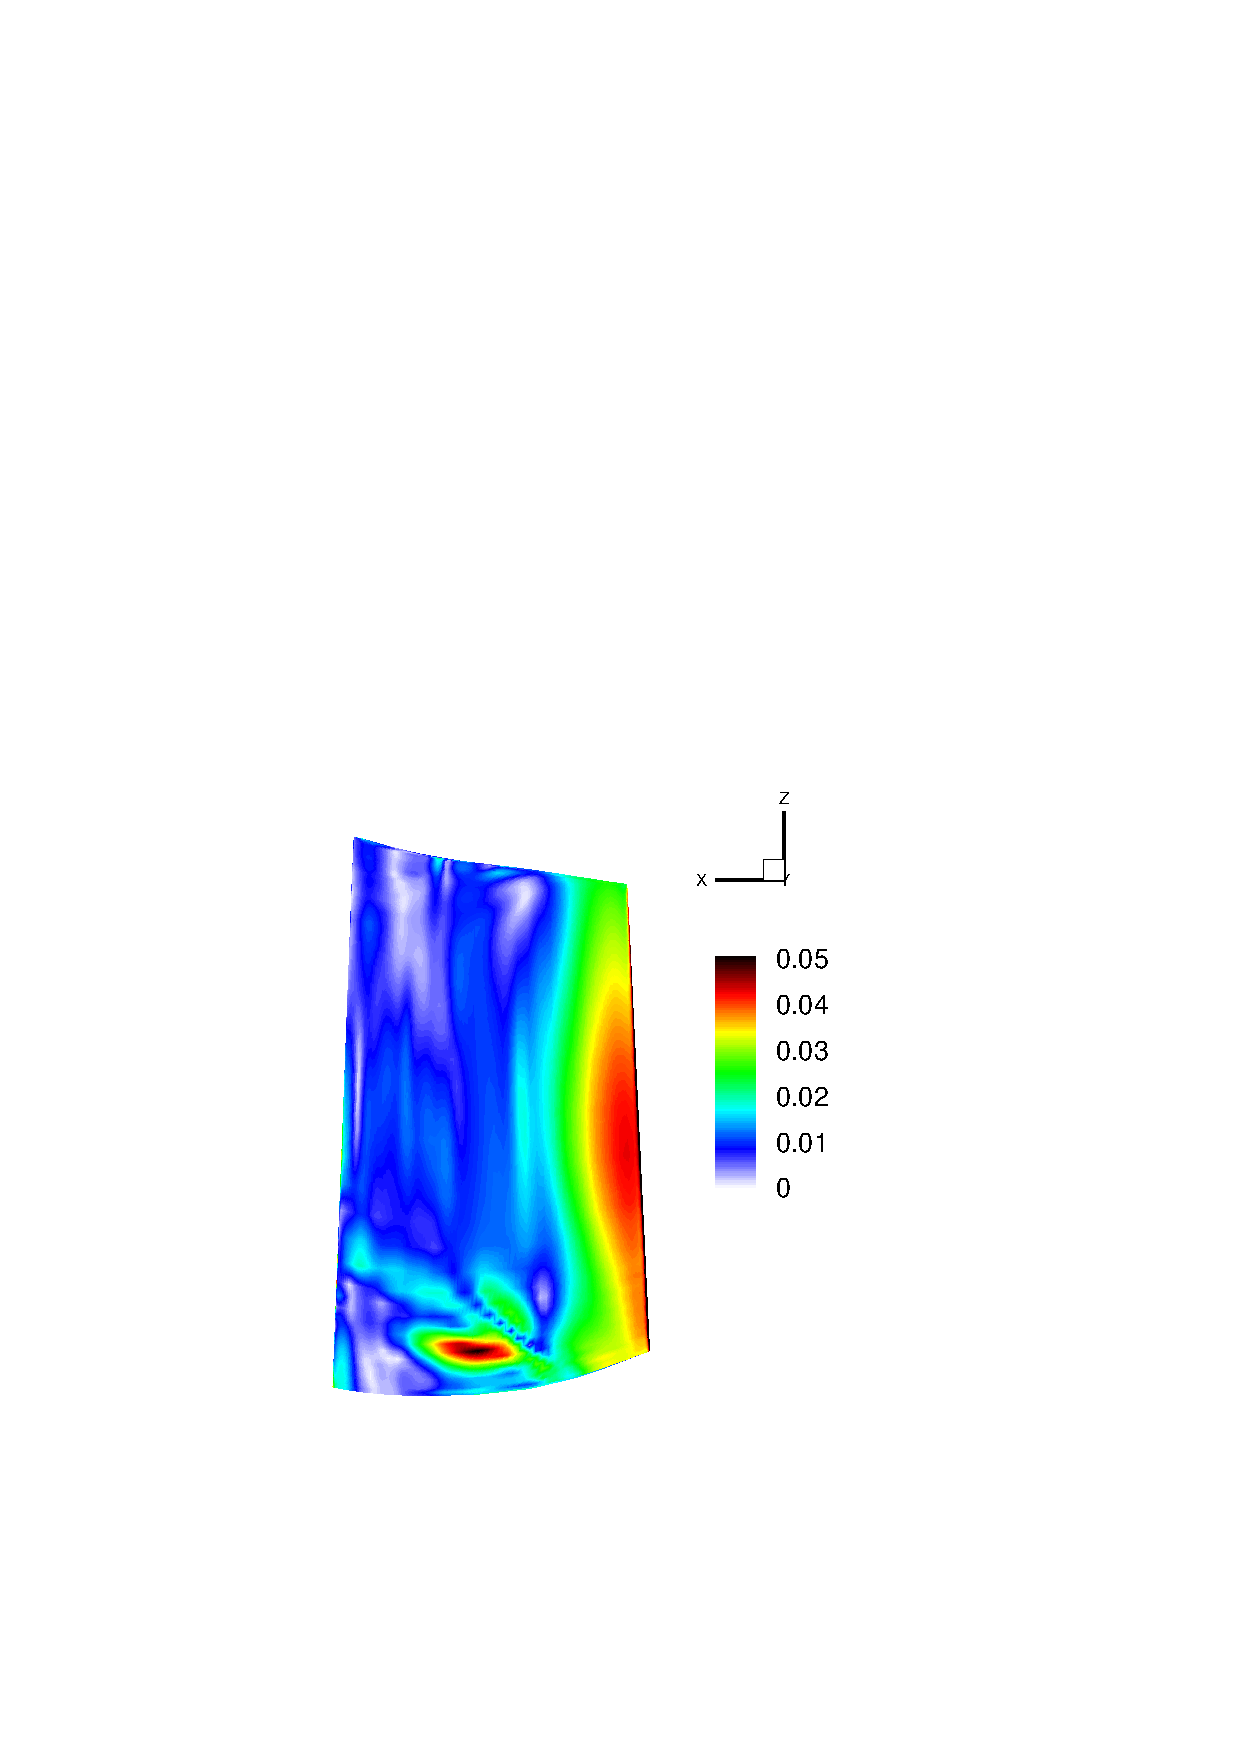
\includegraphics[width=70mm,clip=t]{CHAP_RT27/FIGURE/suctpot1.pdf}}
   \end{tabular}
  \end{center}
  \vspace{-8mm}
  \caption{Unsteady pressure on RT27a rotor blade due to
           potential flow interaction (first Fourier component)}
  \label{rt27_potential1_3d.fig}
\end{figure}
%
 Fig. \ref{rt27_potential1_3d.fig} shows the predicted amplitude
 of the unsteady pressure distribution on the rotor blade due to
 the first Fourier component of the potential flow.

 In the suction side, the unsteady pressure exhibits 3D effects across the
 suction side leg of the horseshoe vortex.
 Fig. \ref{rt27_potential1_3d.fig}b shows that the
 unsteadiness is much higher towards the leading-edge and
 that there is an exponential decay downstream.
 This is compatible with the potential flow theory
 illustrated in appendix \ref{waves.chap}.
 Such a decay rate can also be seen from Fig. \ref{rt27_unsteady3d_1.fig}.

 The unsteady pressure perturbation on the pressure surface
 exhibits a 2D behaviour and it results
 in a `stationary' wave centered at the middle of the blade.
 Such a feature can be seen from Fig.\ref{rt27_unsteady3d_1.fig}
 where the maximum amplitude is located at $x/c\sm{x}\approx -0.75$
 with a phase nearly constant along the axial direction.
 Thus, on the pressure side, the potential-flow unsteadiness does not
 decay exponentially but, on the contrary, seems to follow a different
 behaviour.

 With the help of the unsteady pressure animation, it is possible to
 distinguish two separate regions for the potential flow interaction.
 As the rotor passage moves, it cut the potential flow field in an upstream
 region attached to the NGV outlet and in a rotor passage region
 centered on the pressure surface.
 The upstream interaction, which decays exponentially downstream,
 is responsible for the high perturbations at the leading-edge of
 the blade and it does not interact with the rotor steady pressure field.
 In the region inside the rotor passage, the prescribed potential flow
 interaction from the stator outlet and the potential flow field of the
 rotor itself influence each other.
 Korakianitis \citeyear{Kora:1,Kora:2,Kora:3} showed that this interaction
 is strongly influenced by the stator-to-rotor pitch
 ratio and, consequently, by the inter-blade phase angle as reported in
 Appendix \ref{waves.chap}.
 For equal rotor and stator pitches, the inter-blade phase angle
 becomes $2\pi$. In this scenario, the potential flow interaction affects
 only the leading-edge of the blade while for a larger ratio
 (and smaller inter-blade phase angle)
 the interaction affects the whole of the rotor assembley.

 Although the pressure variation due to the potential-flow interaction
 is a pressure disturbance entering the rotor passages, this pressure
 disturbance does not ``propagate'' downstream the rotor blade at the
 sonic or any other velocity. The potential-flow disturbance is a pressure
 field which is located in the traverse of the rotor assebley; it is affected
 by the potential-flow interaction of the rotor itself, but it does
 not propagate. The interaction between the pressure disturbance and
 the rotor pressure field occurs in the middle of the passage and it
 is located in the pressure side of the blade.

~\newline
 The unsteady pressure perturbations generated by the second Fourier component
 of the potential flow field of the NGV outlet is shown in Fig.
 \ref{rt27_potential2_3d.fig}.
%
\begin{figure}
  \begin{center}
   \begin{tabular}{cc}
     \subfigure[Pressure surface]
       {\hspace{-5mm}
        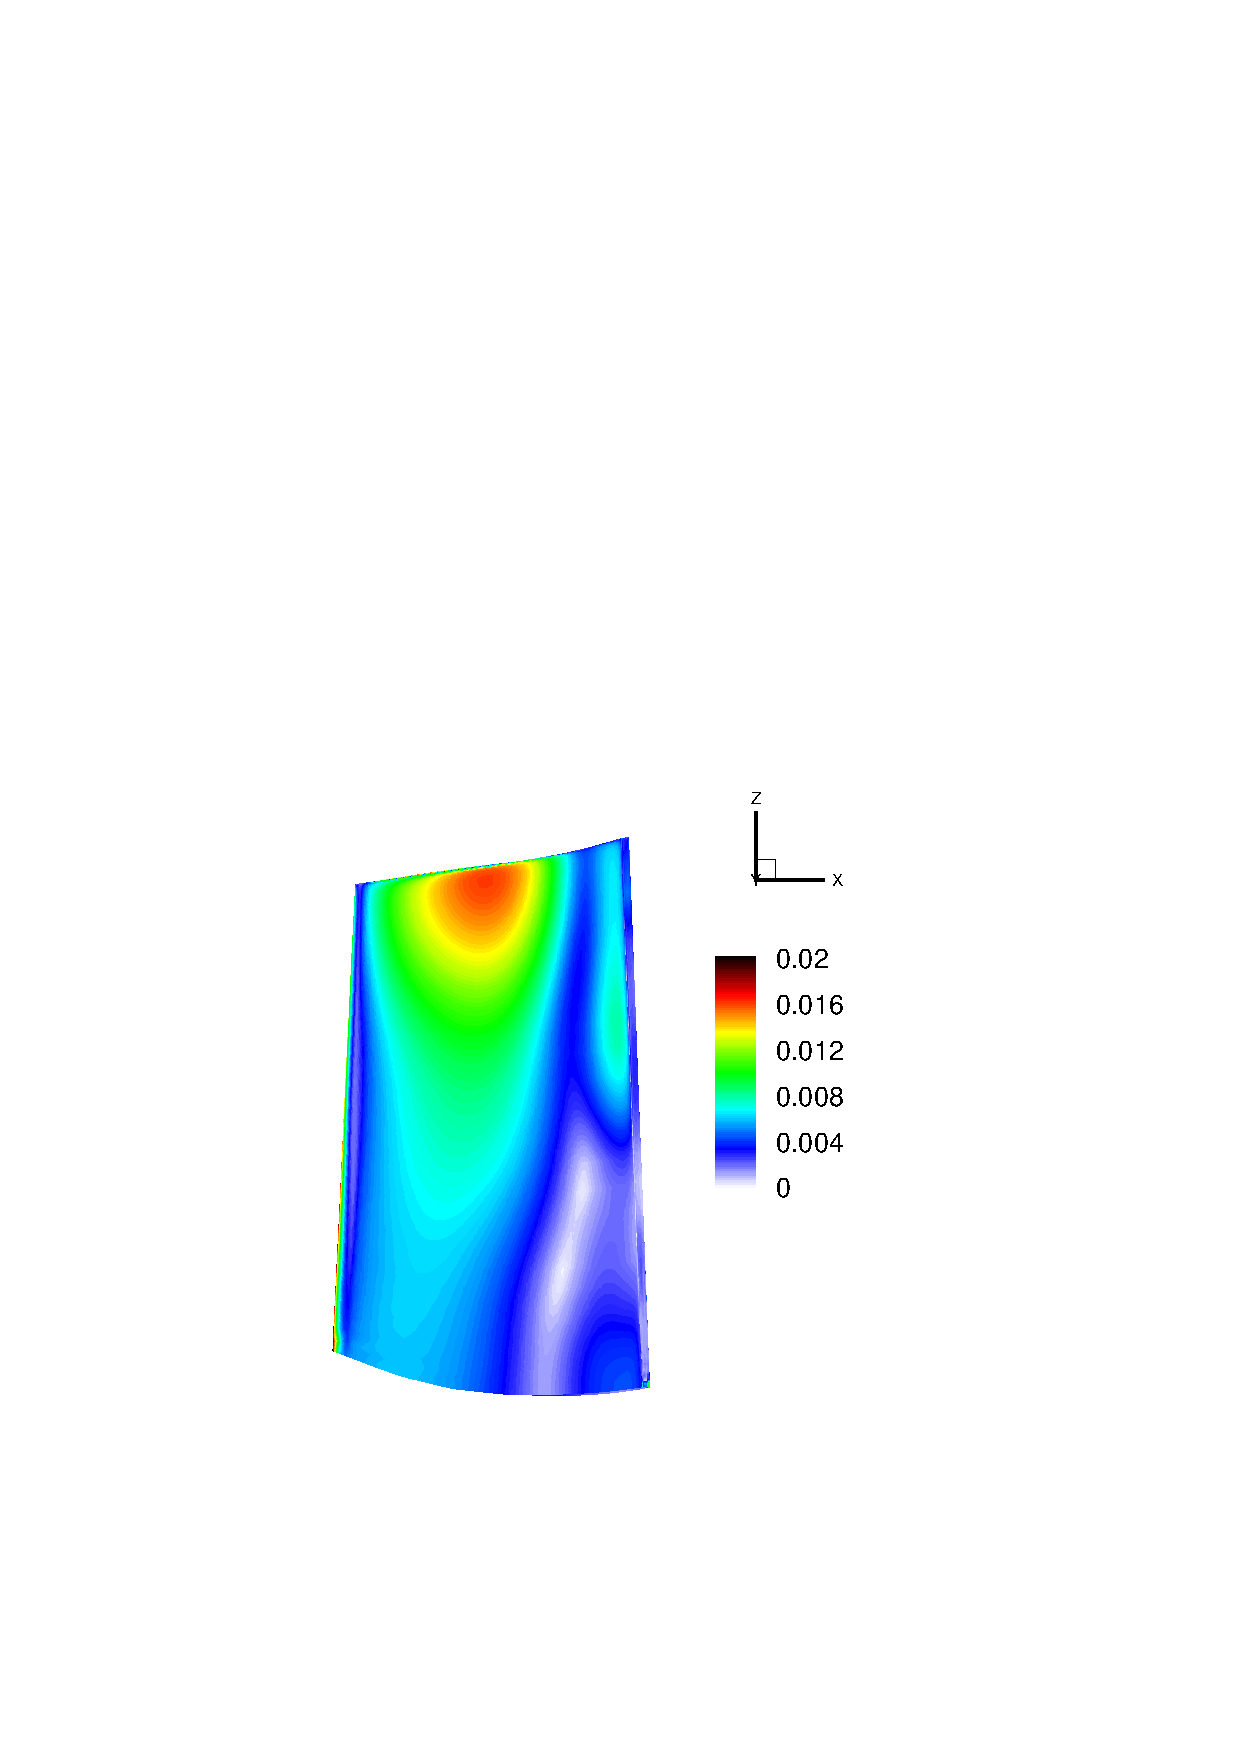
\includegraphics[width=70mm,clip=t]{CHAP_RT27/FIGURE/prespot2.pdf}}
       &
     \subfigure[Suction surface]
       {\hspace{-5mm}
        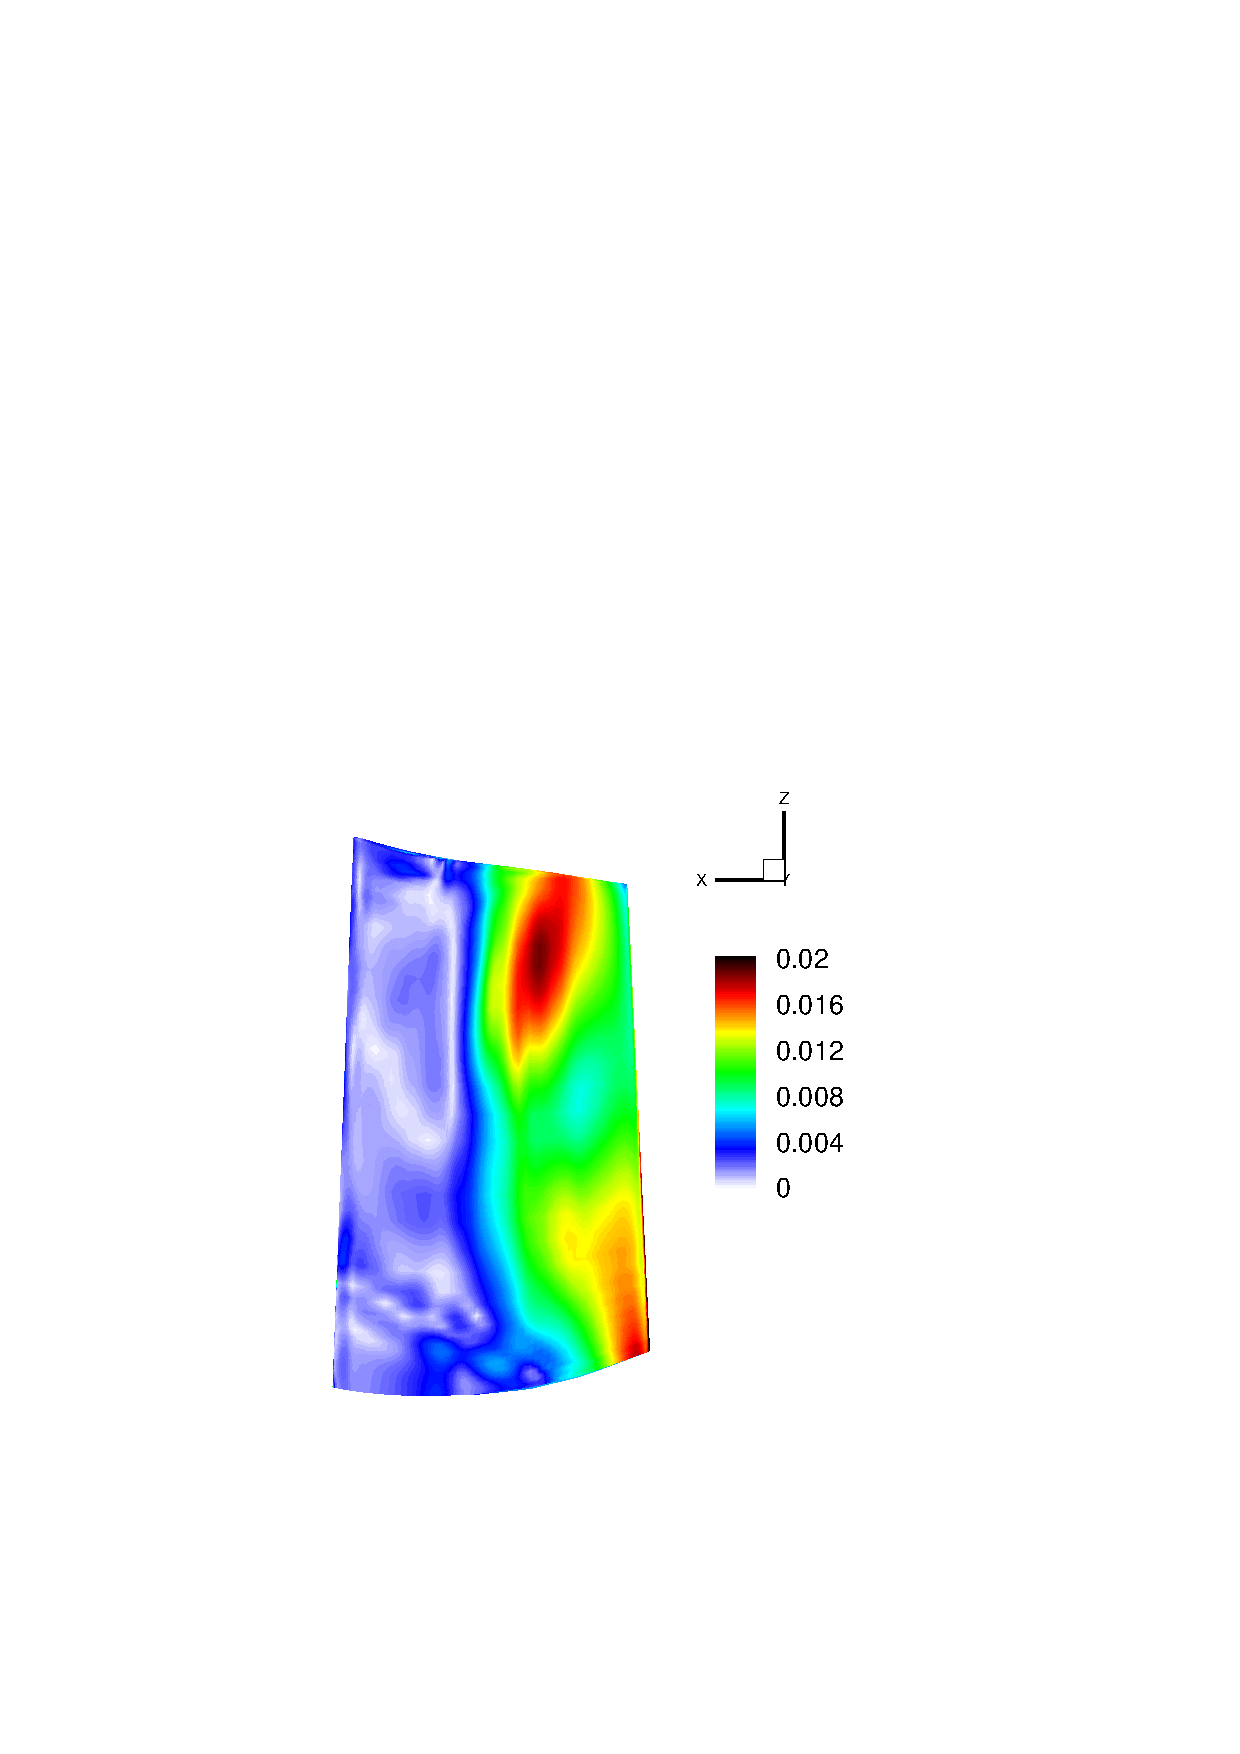
\includegraphics[width=70mm,clip=t]{CHAP_RT27/FIGURE/suctpot2.pdf}}
   \end{tabular}
  \end{center}
  \vspace{-8mm}
  \caption{Unsteady pressure on RT27a rotor blade due to
           potential flow interaction (second Fourier component)}
  \label{rt27_potential2_3d.fig}
\end{figure}
%
 The resulting potential flow interaction shows a large 3D
 effect when compared with the distribution in Fig. \ref{rt27_potential1_3d.fig}.
 The unsteady pressure behaviour, on the other hand, is very similar to that
 previously discussed. The disturbance on the suction
 side decays more rapidly than the first harmonic and this
 is in perfect agreement with the potential flow theory.
 The interaction between the disturbance and the rotor pressure field is
 again visible in the pressure surface of the blade where a
 pressure pulsation is still present.
 However such pulsation on the pressure surface seems to
 possess a propagative behaviour in the spanwise direction.
 From the unsteady pressure animation, it is evident that the
 interaction starts at the blade root, where
 the inlet disturbance is higher (Fig. \ref{rt27_potential2_3d.fig}a),
 and propagates towards the tip section growing in amplitude.

 A possible cause of this propagative 3D effect can
 be attributed to the presence of centrifugal and Coriolis forces
 created by the blade rotation.
 It has been demonstrated by several authors
 (Kerrebrock \citeyearNP{Kerrebrock:1},
  Atassi \& Golubev \citeyearNP{Atassi:1}) that,
 for non-uniform mean flow, such forces deflect
 the fluid motion and couple together the potential
 and vortical modes.
 Becaise of such coumpling neither convected vortical nor
 irrotational acoustic disturbances exist. Instead,
 (i) nearly-convected or vorticity-dominated modal disturbances,
 that contains pressure, and (ii) acoustic or pressure-dominated
 modal disturbances, that contain vorticity, occur
 (Montgomery \& Verdon \citeyearNP{Verdon:3}).
%
%
\subsection{Summary of the main findings}
%
 The unsteady pressure on a 3D HP turbine rotor blade due
 to potential-flow and viscous-wake
 interaction from the upstream NGV was computed using a linear
 flow representation.
 The potential-flow and the viscous-wake from the upstream
 NGV are modelled as inlet distorsions at the rotor-inlet boundary.
 The superimposed solutions for the first (blade passing
 frequency) and second Fourier modes were compared with
 available experimental data. The overall agreement
 was considered to be sadisfactory although the pressure
 side perturbations due to the first Fourier mode were
 overestimated.
 The main conclusions of this unsteady analysis can be summarised
 as follow:
%
\begin{itemize}
%
\item
 The wake-rotor interaction is caracterised by the cutting of
 the NGV wake by the rotor blade. Such a process generates a wake
 segment in the rotor passage which interact with the potential
 flow-field of the rotor itself. The vortical pattern upstream of the
 wake centerline generates an increase in local pressure while
 the the vortical pattern downstream of the wake centerline
 generates a decrease in local pressure.
%
\item
 At mid-heigh section, where the flow is quasi 2D, the perturbations
 due to wake-rotor interaction are higher at the crown of the blade.
 This is true for both the first and second Fourier component.
%
\item
 The perturbation caused by vortical-rotor propagates from inlet towards
 the rotor outlet with the steady-state local fluid velocity.
%
\item
 Two separate regions for the potential-flow interaction can be
 distinguished in the rotor domain. The first region is attached to the stator
 outlet and interacts with the rotor leading-edge. Such interaction is strong
 but decays exponentially dowstream.
 The second region is located in the rotor passage and it is the consequence of
 the interaction between the potential-flow at the rotor inlet and the potential
 flow field of the rotor itself. Such iteraction results in a `stationary'
 pressure wave centered at the middle of the rotor pressure surface.
%
\item
 Such a pressure pulsation on the blade passage is 'stationary' only for
 the first Fourier component. The second Fourier components of the
 potential-flow mode exhibits a propagative radial behaviour although
 for a given radial section it still results in a 'stationary' pulsation.
 This 3D behaviour can be explaned by the presence of
 centrifugal and Coriolis forces which couple together vortical
 and acoustic modes.
%
\item
 The importance of including both potential and vortical disturbances is clearly
 demonstrated. Strong 3D effects for both interactions are
 positioned across the suction side leg of the horseshoe vortex.
%
\end{itemize}
%
